\documentclass[a4paper]{book}
\usepackage[italian]{babel}
\usepackage[utf8]{inputenc}
\usepackage[T1]{fontenc}
\usepackage[sc]{mathpazo} % Palatino!
\linespread{1.05}         % Palatino needs more leading (space between lines)
\usepackage{graphicx}
\usepackage{amsmath}
\usepackage{indentfirst}
\usepackage{amsthm}
\usepackage{amssymb}
\usepackage{booktabs}
\usepackage{listings}
\usepackage{wrapfig}
\usepackage{bbding}
\usepackage{float}
\usepackage[a4paper,top=2.5cm,bottom=2.5cm,left=2cm,right=2cm,bindingoffset=5mm]{geometry}
\usepackage[font=small,format=hang,labelfont={sf,bf}]{caption} % Per un diverso carattere per le didascalie


\newenvironment{esercizio}{\subsection{Esercizio}\sffamily}{}

\author{Ingegnere Pazzo \\ http://ingegnerepazzo.wordpress.com/}
\title{Appunti di Sistemi d'elaborazione dell'informazione \\ (Prima versione)}

\begin{document}

\maketitle
\thanks{Si consiglia di affiancare il materiale presente in questo riassunto agli appunti presi a lezione. Questo perché (ovviamente!) non ho alcuna presunzione di esaustività, né di assoluta correttezza: nonostante una prima revisione, potrebbero infatti essere ancora presenti molti errori e imprecisioni. Si ringrazia il prof. Tullio Salmon Cinotti per avermi permesso di usare, in questi appunti, alcune immagini tratte dalle sue \textit{slides}.}
\tableofcontents
\chapter{Introduzione}
\label{cha:Introduzione}

\section{Cosa determina le prestazioni di un calcolatore}
\label{sec:cosaDeterminaPrestazioni}

Un'architettura di elaborazione\footnote{Faremo costantemente riferimento al modello basato sulla macchina di Von Neumann.} � costituita da tre elementi fondamentali:
\begin{itemize}
\item l'\textbf{ISA} (\textit{Instruction Stack Architecture}), ovvero il set di istruzioni computabile dalla macchina;
\item la \textbf{struttura} (v. esempio in figura \ref{fig:strutturaSchematica}), cio� l'insieme di blocchi interconnessi fra loro che realizza il principio di funzionamento del sistema;
\begin{figure}[!h]
\centering
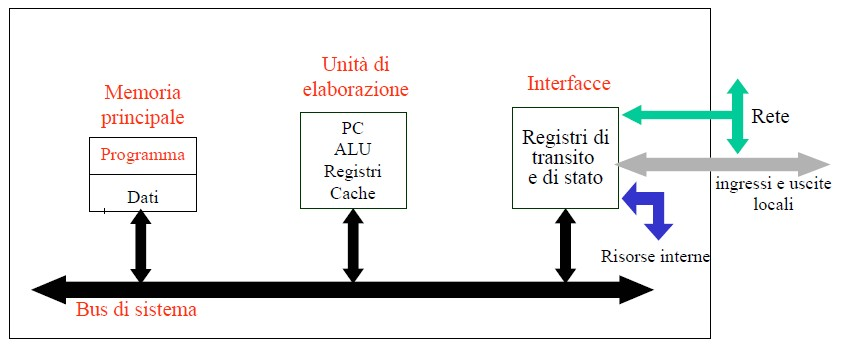
\includegraphics[width=0.8\columnwidth]{img/strutturaSchematica}
\caption{Una schematizzazione essenziale della struttura di un calcolatore}
\label{fig:strutturaSchematica}
\end{figure}
\item la \textbf{realizzazione circuitale} del sistema, cio� com'� fatto "'elettronicamente'".
\end{itemize}

Questi tre elementi impattano significativamente sulle prestazioni del nostro elaboratore, quantificabili attraverso il parametro $CPU_{time}$, cio� il tempo che impiega la macchina ad eseguire un certo \textit{task}:
\[
CPU_{time} = N_{istruzioni} \cdot CPI_{medio} \cdot T_{clock}
\]
Il numero di istruzioni ($N_{istruzioni}$) dipende dell'ISA, il $CPI_{medio}$ dalla struttura hardware del nostro sistema, il $T_{clock}$ (periodo di clock) dalla tecnologia di realizzazione (cio� dall'elettronica sottostante la fabbricazione dell'hardware).

Tecnologia e struttura interna evolvono nell'ottica di aumentare le prestazioni e ridurre il consumo/operazione
elementare. In particolare, si cerca di trovare il miglior compromesso fra potenza e consumo tramite i seguenti accorgimenti:
\begin{itemize}
\item riduzione delle tensioni di alimentazione;
\item definizione di diversi stati di funzionamento in modo da
alimentare selettivamente a divisione di tempo solo i blocchi
istante per istante necessari;
\item variazione della frequenza di funzionamento in funzione del
carico computazionale;
\item variazione della tensione di alimentazione in funzione della
frequenza istantanea di funzionamento;
\item \textit{Power management} esteso all'intero sistema, non solo alla
CPU.
\end{itemize}


\subsection{L'ISA}
\label{sec:isa}

Il linguaggio macchina (L.M.) (detto anche \textit{instruction set architecture} - ISA) � il livello dell'architettura della CPU visibile a chi sviluppa i compilatori e a chi programma in \textit{assembler}. L'ISA � costituita dall'insieme delle istruzioni eseguibili e dal loro formato binario. Con le istruzioni del linguaggio macchina si accede alle risorse interne del calcolatore (memoria, registri, tabelle e descrittori, variabili di stato, \textit{flag}, etc\ldots). Tra le risorse interne al calcolatore, solo quelle accessibili attraverso l'ISA possono essere rese visibili e controllabili dal software.

Per comodit� in generale non rappresenteremo le istruzioni macchina con zeri e uni (cio� come vengono viste dal calcolatore), n� con cifre esadecimali in forma simbolica; il linguaggio che useremo per rappresentare simbolicamente le istruzioni del linguaggio macchina � l'\textit{assembler}.

Le istruzioni prese in pasto da un calcolatore\footnote{In questo paragrafo faremo riferimento all'Intel 8086/8088 oppure al DLX.} hanno una struttura del tipo:
\begin{verbatim}
ADD   ALFA[DI+BX], AL
\end{verbatim}
In questo caso DI+BX � l'indice di ALFA, che � un vettore: l'operazione effettuata consiste nel sommare alla quantit� presente in ALFA[DI+BX] (operando in memoria) la quantit� AL. Con ALFA[DI+BX] indichiamo simbolicamente una posizione in memoria; la memoria, nell'8088, � di 1 MB ($20^{20}$ bit) ed � "'puntata'" da DS (\textit{data segment}, vedi fig. \ref{fig:DSmemoria}), vettore di 20 bit con i 4 bit meno significativi posti a 0: questo significa che � possibile indirizzare le celle di memoria, ampie $2^4 = 16$ byte ciascuna e dette \textit{paragrafi}, con soli 16 bit (4 cifre esadecimali) dei 20 totali.
\begin{figure}[!h]
\centering
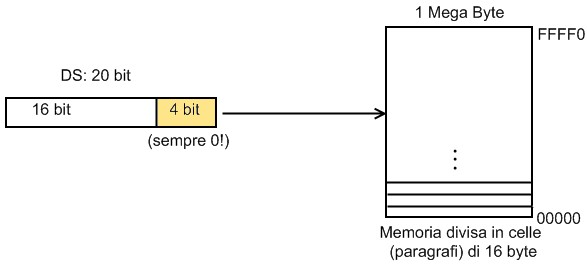
\includegraphics[width=0.7\columnwidth]{img/DSmemoria}
\caption{Struttura della memoria e suddivisione in paragrafi}
\label{fig:DSmemoria}
\end{figure}

Un'altra possibile suddivisione logica della memoria � quella in pagine, ovvero in $2^8$ blocchi di $2^{12}$ byte (vedi fig. \ref{fig:pagineParagrafi}).

\begin{figure}[!h]
\centering
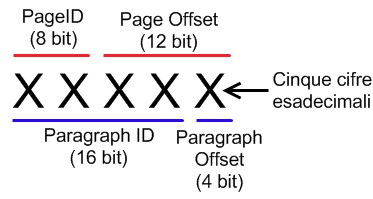
\includegraphics[width=0.4\columnwidth]{img/pagineParagrafi}
\caption{\textit{Base} e \textit{offset} per pagine e paragrafi}
\label{fig:pagineParagrafi}
\end{figure}

Si noti che la divisione in paragrafi e in pagine implica:
\begin{itemize}
\item un metodo di indirizzamento \textit{base} (indirizzo iniziale della cella di memoria) + \textit{offset} (indirizzo all'interno della cella);
\item che � possibile far s� che l'indirizzo di un blocco sia sempre un multiplo della dimensione del blocco stesso (\textit{indirizzi allineati}); questo comporta che, se prendiamo in considerazione il DLX (4 GigaByte di memoria da indirizzare, indirizzi di 32 bit), non necessiteremo di un sommatore a 32 bit per il calcolo dell'indirizzo "'effettivo'" (\textit{base} + \textit{offset}), potendo furbescamente sfruttare il concatenamento di \textit{blockID} + \textit{offset}. \\
Esempio (DLX, $n=32$, indirizzi allineati): devo accedere a una cella di memoria individuata dal \textit{blockID} che, per definizione, ha i $k$ bit meno significativi tutti a zero, e ho bisogno dell'informazione, che chiameremo PIPPO, presente ad un certo \textit{offset} lungo $k$ bit. Per trovare l'indirizzo di PIPPO basta una semplice operazione di concatenamento:
\begin{verbatim}
ind(PIPPO) [n bit] = Block_ID [n-k bit] ## Offset [k bit]
\end{verbatim}
Se invece i blocchi non sono allineati (es. 8088, dove sia la base che l'offset sono a 16 bit, con un DS di 20 bit), oppure se l'offset � maggiore della dimensione del blocco, il sommatore � imprescindibile.
\end{itemize}

Nell'8088 l'offset � calcolato dinamicamente ed � la somma di BX + DI + ALFA (vedi fig. \ref{fig:effectiveAddress}).

\begin{figure}[!h]
\centering
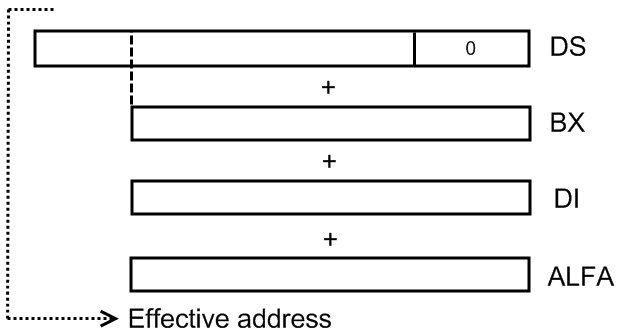
\includegraphics[width=0.5\columnwidth]{img/effectiveAddress}
\caption{Calcolo dell'\textit{effective address}}
\label{fig:effectiveAddress}
\end{figure}

\subsection{Struttura (architettura)}
\label{sec:strutturaArchitettura}

\begin{figure}[!h]
\centering
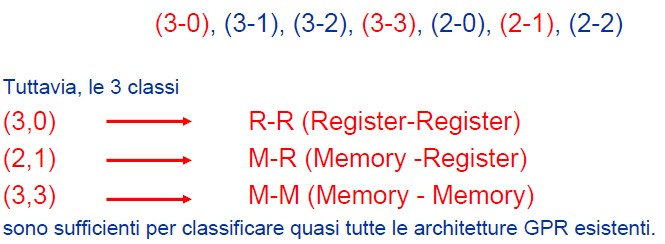
\includegraphics[width=0.7\columnwidth]{img/tipiArchitetture}
\caption{Schema riassuntivo della nomenclatura per tipologie d'architettura}
\label{fig:tipiArchitettura}
\end{figure}

Una macchina che fa uso di due operandi espliciti e di uno in memoria viene detta avente architettura 2-1. 
Esempio di istruzione di macchina 2-1 (detta anche M-R, memoria-registro): 
\begin{verbatim}
ADD   ALFA[DI+BX], AL
\end{verbatim}
Con una singola riga di codice effettuiamo una relativamente numerosa serie di operazioni elementari (memorizzazione, \textit{fetch}, somme, etc\ldots), le quali richiedono molti clock per essere eseguite; dunque:
\[
CPI_{medio}~~ \text{(clock per instruction: ALTO)} ~~~~~~~~~ N_{istruzioni}~~ \text{(numero di istruzioni: BASSO)}
\]
Si parla quindi di architettura CISC (\textit{Complex Instruction Set Computer}). \\

Il DLX ha invece un'architettura 3-0 (detta anche R-R, registro-registro), con istruzioni aventi tre operandi espliciti e nessuno in memoria:
\begin{verbatim}
ADD R5, R6, R7
\end{verbatim}
Per prelevare e depositare in memoria ci si appoggia quindi alle istruzioni di LOAD e STORE. \\

L'architettura influisce tantissimo sia sulle prestazioni che sul generale funzionamento del calcolatore: infine, con una stessa ISA possono sussistere strutture diversissime (ad esempio pu� essere pi� o meno realizzabile la \textit{pipeline} piuttosto che la struttura ad esecuzione sequenziale, etc\ldots).

\section{Tipi di istruzioni}
\label{sec:tipiIstruzioni}

In questo paragrafo considereremo l'architettura del DLX ($2^{32}$ byte di indirizzamento).

\begin{figure}[!h]
\centering
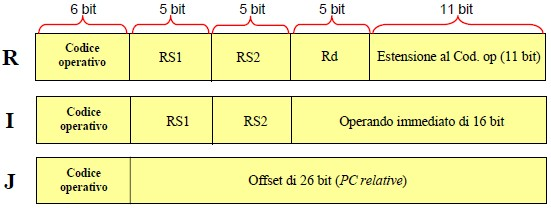
\includegraphics[width=0.65\columnwidth]{img/TipiIstruzioni}
\caption{Tipologie d'istruzione}
\label{fig:TipiIstruzioni}
\end{figure}
\begin{figure}[!h]
\centering
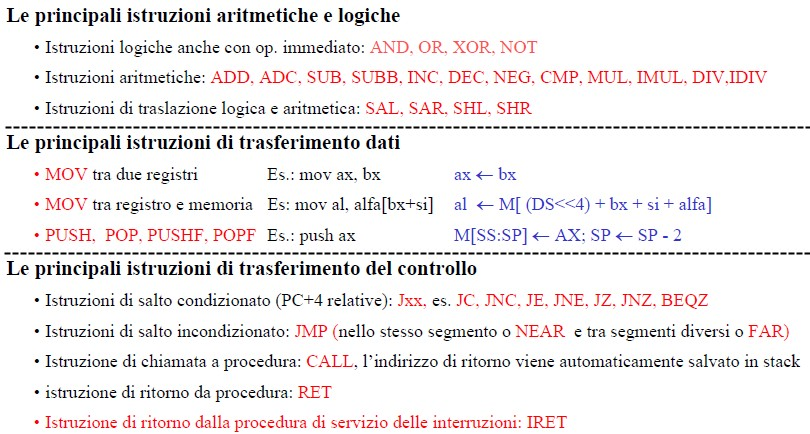
\includegraphics[width=\columnwidth]{img/listaistruzioni}
\caption{Schema di massima dei principali tipi di istruzioni}
\label{fig:listaistruzioni}
\end{figure}

\subsection{Di tipo R}
\label{sec:tipoR}

Si tratta delle tipiche istruzioni ALU, in cui sono coinvolti tre registri. Esempio:
\begin{verbatim}
ADD   R1, R2, R3
\end{verbatim}

\subsection{Di tipo I}
\label{sec:tipoI}

Sono le istruzioni con operando immediato (cui sono riservati 16 bit in complemento a 2, per un range - quindi - che va da -32K a 32K-1), come
\begin{itemize}
\item \textit{Load}/\textit{Store}. Ad esempio:
\begin{verbatim}
LB    R5, 20(R6)
\end{verbatim}
Questa istruzione\footnote{Equivalente a 
\[
R5_{[7\ldots 0]} \Leftarrow M[R6+20]
\]} mette in R5 il contenuto della cella di memoria il cui indirizzo � il contenuto del registro R6 incrementato di 20.
Oppure:
\begin{verbatim}
LDRS   ALFA(R6)
\end{verbatim}
ALFA � detta \textit{parte fissa}, mentre il contenuto di R6 � la \textit{parte variabile}: quel che si fa � accedere all'R6-simo elemento del vettore ALFA ed effettuarne il \textit{load}.
\item \textit{Branch condizionate}, ovvero salto \textbf{condizionato}. Esempio\footnote{Si tratta di una \textit{Branch Not Equal Zero}: in pratica, se in PIPPO vi � il valore 3, dobbiamo andare a PC+3 (per questo si dice che � un'istruzione \textit{PC-relative}).}
\begin{verbatim}
BNEZ   R5, PIPPO
\end{verbatim}
Altri esempi (\textit{Branch Not Equal Zero})\footnote{Se R10 � diverso da 0 saltiamo a PIPPO.}:
\begin{verbatim}
BNEQZ   R10, PIPPO
\end{verbatim}
Che � equivalente a (\textit{Jump Equal})\footnote{Se R5=R6 saltiamo a PIPPO.}
\begin{verbatim}
JEQ    R5, R6, PIPPO
\end{verbatim}
se R10 � stato ricavato con questa istruzione (\textit{Set Equal Zero})\footnote{Mettiamo in R10 il risultato del confronto fra gli operandi R5 e R6.}:
\begin{verbatim}
SEQ    R10, R5, R6
\end{verbatim}

\item \textit{Jump Register} (JR);
\item \textit{Jump and Link register} (JALR);
\item ALU con operando immediato, ad esempio:
\begin{verbatim}
ADDI   R1, R2, 3
\end{verbatim}
Per questo tipo di operazioni viene coinvolta la ALU, che prende in pasto due operandi da 32 bit: siccome l'operando immediato � una quantit� a 16 bit, i rimanenti bit sono rappresentati dal bit del segno ripetuto 16 volte.
\end{itemize}

\subsection{Di tipo J}
\label{sec:tipoJ}

Si tratta di istruzioni di \textit{jump} (salto \textbf{incondizionato}), ancora una volta \textit{PC-relative} con l'operando immediato presente nella finestra\footnote{Ampia 64 MB e centrata sul PC.}:
\[
-2^{25} \Rightarrow 2^{25}-1
\]
Quando � necessario effettuare un salto (\textit{jump}) l'indirizzo di ritorno viene salvato nel registro R31 ma, se per qualche motivo nel frattempo venisse eseguita un'altra procedura, l'indirizzo di ritorno in R31 verrebbe sovrascritto e noi saremmo fregati. Quanto detto si riflette nell'assenza del cosiddetto \textit{nesting}, cosicch� deve curarsene il programmatore (facendo uso, ad esempio, di altri registri come R30). Se teniamo conto di questo aspetto, come ci regoliamo con gli \textit{interrupt}? Gli \textit{interrupt} sono chiamate a procedure "'implicite'", scatenate da un evento o un dispositivo esterno (come ad esempio una periferica): l'indirizzo di ritorno, in questo caso, non viene salvato in R31 bens� in IAR(\textit{Interrupt Address Register}). 
IAR e R31 sono quindi i due registri deputati al salvataggio degli indirizzi di ritorno.

Come facciamo per regolare il ritorno dalle eccezioni (ad es. divisione per zero, al sopraggiungere della quale la CPU si arrabbia e si sfoga sull'utente generando - appunto - un'eccezione)? Esiste un'istruzione ad-hoc
\begin{verbatim}
RFE   (Return From Exception)
\end{verbatim}
all'esecuzione della quale si salva l'indirizzo corrente in IAR. 

\chapter{\textit{Pipeline}}
\label{cha:pipeline}

\begin{figure}[!h]
\centering
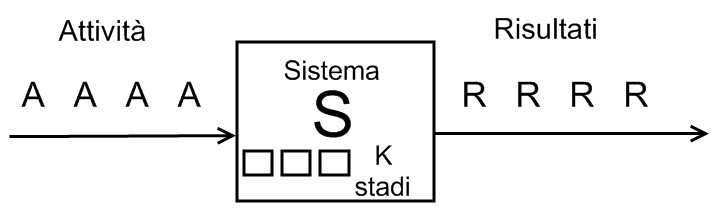
\includegraphics[width=0.5\columnwidth]{img/principioPipeline}
\caption{Schema di principio della \textit{pipeline}}
\label{fig:principioPipeline}
\end{figure}

Il \textit{pipelining} è oggi la principale tecnica di base impiegata per rendere performante una CPU. L'idea alla base del \textit{pipelining} è generale, e trova applicazione in molteplici settori dell'industria (linee di produzione, oleodotti, etc\ldots). Prendiamo in considerazione un generico sistema S che debba e eseguire alcune attività A (vedi fig. \ref{fig:principioPipeline}). Si chiama \textit{latenza (latency)} il tempo che intercorre fra l'inizio ed il completamento della generica attività A, mentre il \textit{throughput} è frequenza con cui vengono completate le attività.

Il \textit{pipelining} non riduce il tempo necessario al completamento di una singola attività, tuttavia incrementa il \textit{throughput} tante volte quanti sono gli stati della \textit{pipeline} (ma solo in un caso ideale!!).

\begin{figure}[!h]
\centering
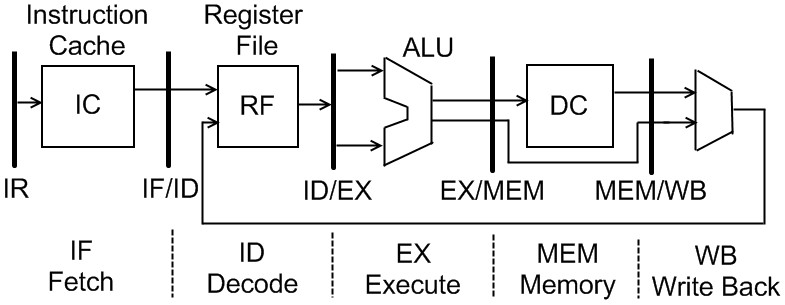
\includegraphics[width=0.7\columnwidth]{img/pipeline}
\caption{Struttura della \textit{pipeline} del DLX}
\label{fig:pipelineDLX}
\end{figure}

Nella \textit{pipeline} del DLX sono presenti cinque fasi principali (ogni fase rappresenta un particolare stadio, vedi fig. \ref{fig:pipelineDLX}):
\begin{itemize}
\item IF: \textit{Instruction Fetch}. Si legge in memoria qual è la prossima istruzione da eseguire;
\item ID: \textit{Instruction Decode}. Si leggono gli operandi sorgenti e si decodifica l'istruzione per capire cosa effettivamente dev'essere fatto;
\item EX: \textit{Execute}. In tale fase viene coinvolta la ALU e vengono effettuate le operazioni richieste dall'istruzione.
\item MEM: \textit{Memory Access}. Si memorizzano (eventualmente) i risultati della fase di EX.
\item WB: \textit{Write Back}. Si scrivono i risultati nel \textit{register file}\footnote{Memoria presente all'interno della CPU.}.

Purtroppo una \textit{pipeline} è suscettibile a stalli (vedi fig. \ref{fig:stallo}): gli stalli si generano quando si necessita di un dato che deve tuttavia ancora essere aggiornato con il suo corretto valore. Con gli stalli abbiamo quindi momenti in cui la CPU è bloccata (\textit{pipeline bloccante}) e impossibilitata ad eseguire nuove fasi delle varie istruzioni in quanto manca uno degli operandi: a causa di ciò, il $CPU_{time}$ della \textit{pipeline} non è pari al numero di istruzioni (come nel caso ideale), bensì pari a:
\[
CPU_{time} = 4 + N_{istruzioni}  + N_{stalli}
\]
Si noti che l'addendo $4$ si riferisce al numero di clock necessari a riempire la \textit{pipeline}. Risulta evidente che il numero di stalli influisce notevolmente sulle prestazioni: più stalliamo e più clock impieghiamo a completare una certa serie di operazioni. Infatti, se calcoliamo il cosiddetto CPI (\textit{Clock Per Instruction}) abbiamo:
\[
CPI_{medio}=\dfrac{4+N_{istruzioni}+N_{Stalli}}{N_{istruzioni}} ~~~
\mathop  \simeq \limits_{N_{Istruzioni} {\text{ alto}}} 
 ~~~
 1+\dfrac{N_{Stalli}}{N_{Istruzioni}}
\]

\begin{figure}[!h]
\centering
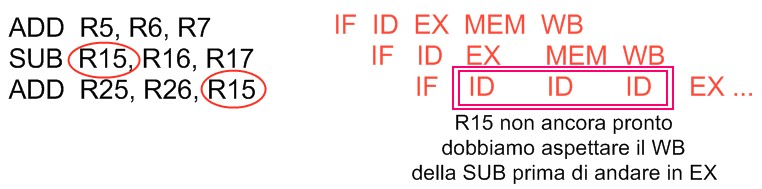
\includegraphics[width=0.8\columnwidth]{img/stallo}
\caption{Il meccanismo dello stallo}
\label{fig:stallo}
\end{figure}

\end{itemize}

\section{Miglioramenti alla \textit{pipeline}}
\label{sec:pipelineMiglioramenti}

Una possibile scelta per migliorare il funzionamento della \textit{pipeline} può essere quella di utilizzare più unità funzionali per ogni stadio (ad esempio più ALU). In tal caso si parla di \textit{macchina superscalare}.
Si può anche pensare di evitare lo stallo eseguendo, mentre un dato richiesto deve ancora aggiornarsi, un'istruzione successiva priva di \textit{alee} ("'dipendenze'"): questo accorgimento rende la pipeline\textit{ non bloccante}. 
Esempio:
\begin{verbatim}
ADD   R15, R16, R17
LD    R15, PIPPO(R16)
AND   R15, R16, R17
\end{verbatim}
Purtroppo qui non posso fare a meno di stallare, tuttavia posso eseguire eventuali istruzioni successive intanto che le tre illustrate vengono eseguite (OOO Execution, \textit{Out Of Order Execution}).

C'è inoltre da tener presente un aspetto importante: non tutti gli stadi vengono impegnati per un singolo clock. Istruzioni aritmetiche coi \textit{floating point} e/o altri tipi di operazioni piuttosto complesse possono richiedere, ad esempio, una permanenza nello stadio EX molto più duratura rispetto ad altre istruzioni.
Risulta quindi importante scoprire quale possa essere un buon metodo per rilevare possibili dipendenze, per risolvere le \textit{alee} e per individuare quindi le possibili situazioni di incoerenza fra i dati. Ad esempio, se prendiamo in considerazione le seguenti istruzioni
\begin{verbatim}
SUB   R15, R16, R17
AND   R25, R26, R15
\end{verbatim}
Questa dicitura è equivalente a:
\begin{verbatim}
R25 = R26 + (R16 - R17)
\end{verbatim} 
\begin{figure}[!h]
\centering
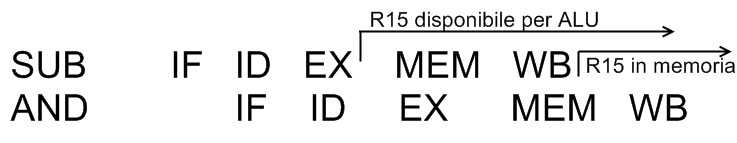
\includegraphics[width=0.7\columnwidth]{img/pipelineEsempio1}
\caption{}
\label{fig:pipelineEsempio1}
\end{figure}
In questo caso il risultato della SUB è necessario alla AND ma non vi sono alee se tali istruzioni vengono eseguite in sequenza (vedi fig. \ref{fig:pipelineEsempio1}): infatti è possibile retrazionare il registro EX-MEM verso la ALU (vedi fig. \ref{fig:retroazionamentoMux}).
\begin{figure}[!h]
\centering
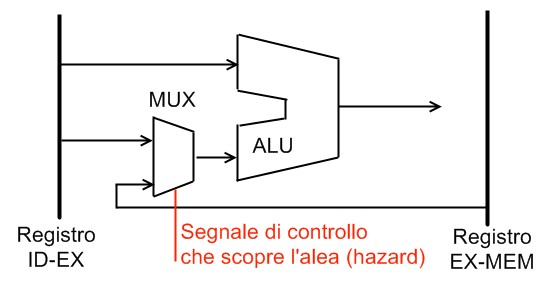
\includegraphics[width=0.6\columnwidth]{img/retroazionamentoMux}
\caption{Meccanismo di retroazione e segnale di controllo}
\label{fig:retroazionamentoMux}
\end{figure}
Risulta quindi necessaria una \textit{Hazard Detection Unit} per scoprire se ci sia l'alea o meno: essa deve gestire il segnale di controllo del MUX (vedi fig. \ref{fig:pipelineEsempio1}) bypassando il \textit{register file}\footnote{In caso contrario avremmo dovuto attendere la fase di WB.}. Questo permette di risparmiare notevoli clock altrimenti persi a causa di stalli.

\begin{figure}[!h]
\centering
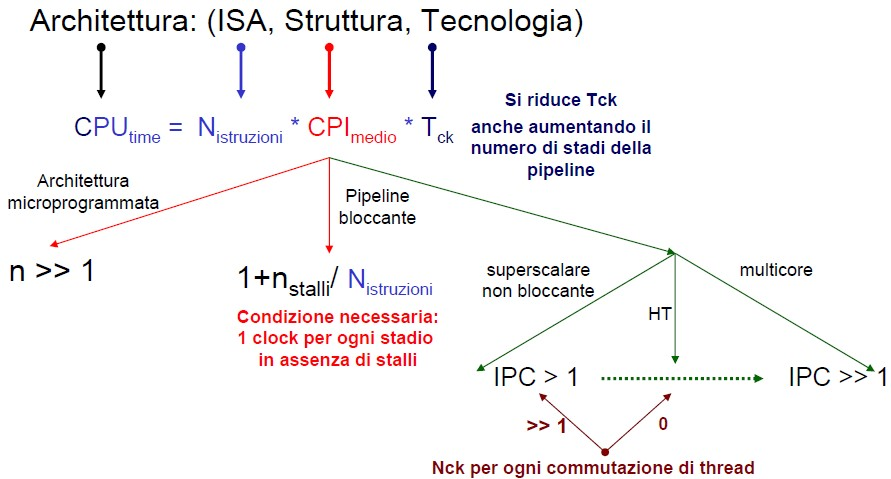
\includegraphics[width=\columnwidth]{img/schemaRiassuntivoArchitetture}
\caption{Schema riassuntivo delle scelte architetturali}
\label{fig:schemaRiassuntivoArchitetture}
\end{figure}

\section{\textit{Pipeline} con stadi a ciclo singolo}
\label{sec:pipelineStadiCicloSingolo}

Prendiamo in considerazione una \textit{pipeline} a ciclo singolo, come quella in figura \ref{fig:pipelineDLX}. Supponendo che il ritardo fra i diversi stadi sia pari a $t_{si}$ la frequenza di clock è vincolata dalla seguente relazione:
\[
t_{ck} \geq 
\mathop {\max }\limits_i \left( {t_{si}  + \underbrace {t_{CHOV\max } }_{{\text{CHOV  = }}{\text{ clock high out valid}}} + \underbrace {t_{SU\min } }_{{\text{SU  =  set up}}}} \right)
\]
In questa relazione
\begin{itemize}
\item $t_{CHOV\max}$ è il massimo ritardo dei registri prima che il dato sia valido in uscita;
\item $t_{SU\min}$ è il tempo di \textit{set-up} minimo (il dato deve rimanere costante).
\end{itemize}

E se volessimo andare più forte con la frequenza di clock (e quindi abbassare $t_{ck}$)? Abbiamo due possibilità d'azione:
\begin{enumerate}
\item Adottiamo una tecnologia migliore.
\item A parità di tecnologia poniamo dei registri all'interno di ogni stato (architettura \textit{Super-Pipelined}, vedi fig. \ref{fig:superpipeline}).
\end{enumerate}
\begin{figure}[!h]
\centering
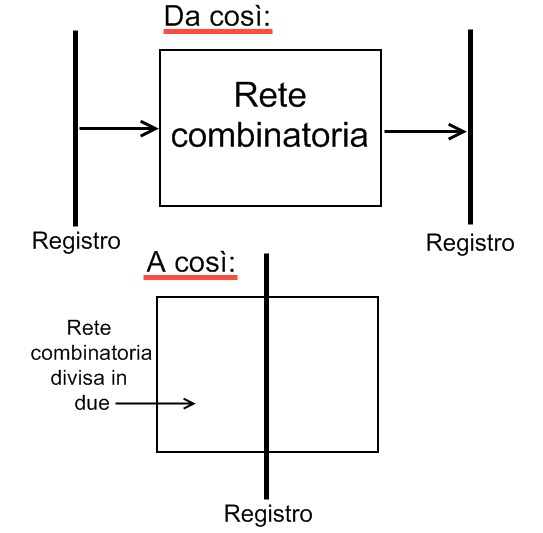
\includegraphics[width=0.5\columnwidth]{img/superpipeline}
\caption{Principio dell'architettura \textit{Super-Pipelined}}
\label{fig:superpipeline}
\end{figure}

\section{Alee}
\label{sec:alee}

\subsection{Alea strutturale}
\label{sec:aleaStrutturale}

Esistono operazioni (come la FDIV, FMUL o FADD, che agiscono su numeri \textit{float}) in grado di impegnare lo stadio EX per molti cicli di clock, compromettendo con reiterati stalli le prestazioni della macchina. Si parla, in questo caso, di \textit{alea strutturale}: a causa degli stalli indotti da tale tipo di alea, uno stadio impegnato per $n$ cicli è in grado di bloccare la \textit{pipeline} per $n-1$ periodi di clock (fino, cioè, al definitivo completamento del calcolo da effettuare). Molte alee strutturali possono quindi far drammaticamente crollare la velocità della nostra \textit{pipeline} con stadio a ciclo singolo mentre, viceversa, se esse non sussistessero sarebbe possibile effettuare molte più istruzioni. Supponendo ad esempio di dover fare 1 DIV (40 clock ciascuna), 10 FADD (4 clock ciascuna) e 40 AND (1 clock ciascuna), impiegheremmo $\{\max \left( {1 \cdot 40,10 \cdot 4,40 \cdot 1} \right)\} = 40$ clock contro i $40+10+1=51$ dei quali avremmo bisogno nel caso di unica unità funzionale: lo \textit{speed-up} della \textit{pipeline} multiciclo è quindi notevole. 

Per ridurre o eliminare gli stalli si può quindi scegliere di implementare \textit{pipeline} con più unità multiciclo in parallelo all'unità di esecuzione intera (vedi fig. \ref{fig:multicycle}). In questo modo è possibile effettuare operazioni diverse in parallelo, guadagnando notevolmente in prestazioni: 

\begin{figure}[!h]
\centering
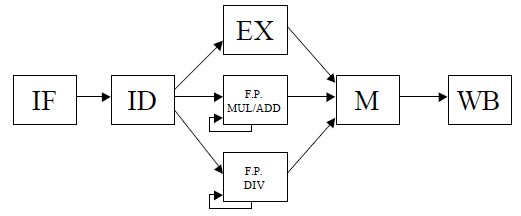
\includegraphics[width=0.55\columnwidth]{img/multicycle}
\caption{Pipeline del DLX con stadi \textit{multicyle} in parallelo}
\label{fig:multicycle}
\end{figure}

\begin{figure}[!h]
\centering
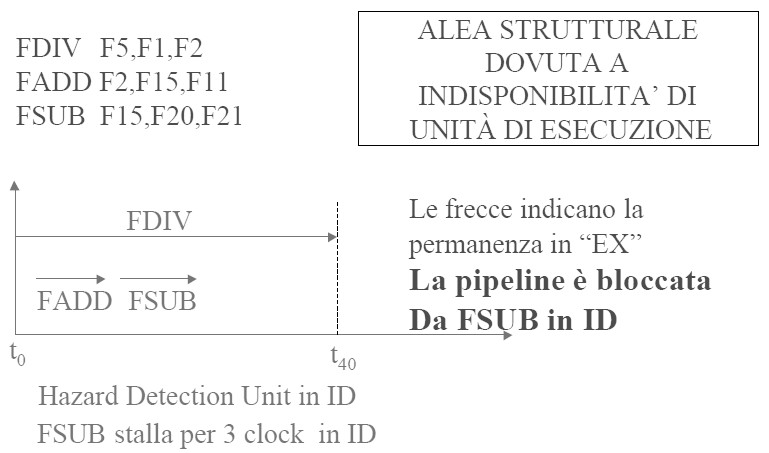
\includegraphics[width=0.7\columnwidth]{img/aleaStrutturale}
\caption{Meccanismo dell'alea strutturale}
\label{fig:aleaStrutturale}
\end{figure}

\subsection{Alea di dato, alee WAW, WAR, RAW}
\label{sec:aleaDato}

Di parla di \textit{alea di dato} (o \textit{alea RAW}, \textit{Read After Write}\footnote{Leggendo oltre si capirà anche il perché di questa denominazione: devo infatti leggere il nuovo dato dopo averlo scritto (calcolato).}) quando, per proseguire, si ha bisogno di un dato che sta per essere calcolato ma impiega molti clock costringendoci ad aspettare. Questo problema può essere parzialmente risolto con l'accelerazione apportata dalla \textit{pipeline multiciclo} (vedi par. \ref{sec:aleaStrutturale}), tuttavia è possibile fare anche di meglio: si può infatti ovviare al problema eseguendo le istruzioni fuori ordine (OOO = \textit{Out Of Order}), effettuando cioè istruzioni successive a quella che sarebbe obbligatorio fare se agissimo in maniera perfettamente sequenziale nel mentre il dato di cui abbiamo bisogno viene calcolato\footnote{"'Devo aspettare che mi arrivi il dato? Nel frattempo faccio altro, sennò starei lì ad oziare.'"}.

\begin{figure}[!h]
\centering
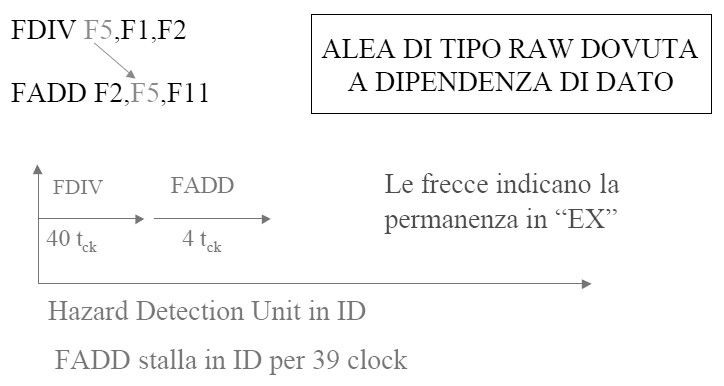
\includegraphics[width=0.7\columnwidth]{img/aleaDato}
\caption{Meccanismo dell'alea RAW (o di dato)}
\label{fig:aleaDato}
\end{figure}

Attenzione! Non si possono invertire le istruzioni a cuor leggero: si rischia infatti di cadere nello stesso errore dal quale cerchiamo di sfuggire, eseguendo cioè istruzioni non effettuabili avendo noi bisogno del dato aggiornato (che è in calcolo)! Il completamento fuori ordine può inoltre rendere imprecisa la gestione delle
eccezioni; ne consegue una esecuzione non corretta del codice, con possibilità di perdere informazioni in modo irrecuperabile. Da qui la necessità di un metodo per capire se sia possibile invertire l'esecuzione di due particolari operazioni, di una modalità - ovvero - di \emph{estrarre il parallelismo intrinseco del codice}\footnote{Ooooooohhh... :-o} \footnote{Detto anche ILP, \textit{Instruction Level Parallelism}.}: in soldoni, devo poter estrarre le dipendenze, le quali hanno tre modi di manifestarsi:
\begin{itemize}
\item \textbf{dipendenza di dato}: già vista poco sopra (par. \ref{sec:aleaDato});
\item \textbf{dipendenza di nome}: due istruzioni usano lo stesso registro ma senza passaggio di dati;
\item \textbf{dipendenza di controllo}: caso suddivisibile in \textit{antidipendenza}, che si verifica "'anticipando'" un'istruzione e rischiando quindi di scrivere su un registro coinvolto in un'operazione precedente, come nel seguente codice
\begin{verbatim}
FADD    F10, F5, F3
FDIV    F5, F1, F1
\end{verbatim}
e \textit{dipendenza d'uscita}, quando un registro contiene il risultato di due operazioni differenti, come accade nelle seguenti righe di assembler:
\begin{verbatim}
FADD    F5, F26, F3
FDIV    F5, F1, F1
\end{verbatim}

L'antidipendenza si manifesta nella cosiddetta alea \textit{Write After Read} (WAR), la quale comporta che il flusso nella \textit{pipeline} non possa proseguire in quanto si deve scrivere su un registro che una istruzione precedente deve leggere ma non ha ancora letto. Fortunatamente le alee WAR non sono possibili in quanto gli operandi
sono sempre letti in nella fase ID, quindi è impossibile che, quando si legge un operando, l'istruzione successiva
l'abbia già aggiornato.

La dipendenza d'uscita, invece, comporta l'alea \textit{Write After Write} (WAW), che si ha quando il flusso nella \textit{pipeline} non può proseguire in quanto una istruzione precedente deve ancora scrivere su un registro che anche
l'istruzione corrente deve aggiornare.
\begin{figure}[!h]
\centering
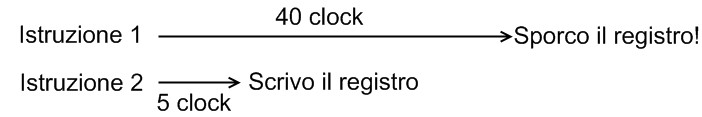
\includegraphics[width=0.7\columnwidth]{img/areaWAW}
\caption{L'alea WAW}
\label{fig:areaWAW}
\end{figure}
Come risolvere l'erronea scrittura di un registro (vedi fig. \ref{fig:areaWAW})? Possiamo pensare di intimare alla prima istruzione di non aggiornare F5 (in alcuni casi le alee WAW si possono eliminare inibendo il
completamento dell'istruzione che determina il malfunzionamento), potremmo effettuare qualche altra istruzione tra la prima e la seconda oppure, se proprio non abbiamo scelta, non ci rimarrà che stallare. In particolare, si dice che una \textit{pipeline} gestisce le eccezioni in modo preciso se essa può essere fermata in modo che tutte le istruzioni precedenti l'istruzione in cui l'eccezione si è verificata siano completate, mentre tutte le istruzioni successive non modifichino lo stato della CPU prima che l'eccezione sia stata servita.
\end{itemize}

In alcuni casi le alee possono rivelarsi davvero pervasive (vedi fig. \ref{fig:aleeABalusa}).
\begin{figure}[!h]
\centering
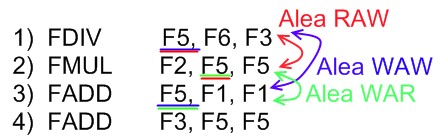
\includegraphics[width=0.5\columnwidth]{img/aleeABalusa}
\caption{Sequenza non indifferente di alee}
\label{fig:aleeABalusa}
\end{figure}
Per evitare situazioni erronee si effettua la fase di \textit{fetch} in sequenza e poi l'ordine viene stabilito dal microprocessore in base alle alee: il criterio è quello di eseguire le istruzioni nell'ordine in cui si hanno a disposizione gli operandi (modalità di tipo \textit{data flow}).
Questo comporta l'essere in grado di poter rinominare i registri (\textit{register renaming}) con valori temporanei (vedi fig. \ref{fig:aleeABalusa2}).
\begin{figure}[!h]
\centering
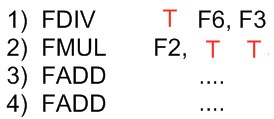
\includegraphics[width=0.3\columnwidth]{img/aleeABalusa2}
\caption{\textit{Register renaming}}
\label{fig:aleeABalusa2}
\end{figure}

\subsection{Alee di controllo}
\label{sec:aleeControllo}

Si hanno quando una delle istruzioni comporta il trasferimento di controllo.
Esempio:
\begin{verbatim}
BEQZ    R6, PIPPO
ADD     R6, R7, R8
\end{verbatim}
Queste istruzioni non possono essere eseguite in parallelo: prima va verificata la condizione, poi si calcola dove si deve saltare e infine si valuta se saltare oppure no. Una politica spesso adottata dai processori è quella di \textit{predire di non saltare}, ovvero supporre che non sarà necessario effettuare la \textit{branch}: questa scelta rientra nell'ambito della cosiddetta \textit{esecuzione speculativa} e comporta l'eseguire in maniera "'provvisoria'" istruzioni successive a quella del salto, per poi darle per buone in caso di corretta previsione oppure scartarle nel caso di predizione sbagliata (\textit{misprediction}).

\begin{figure}[!h]
\centering
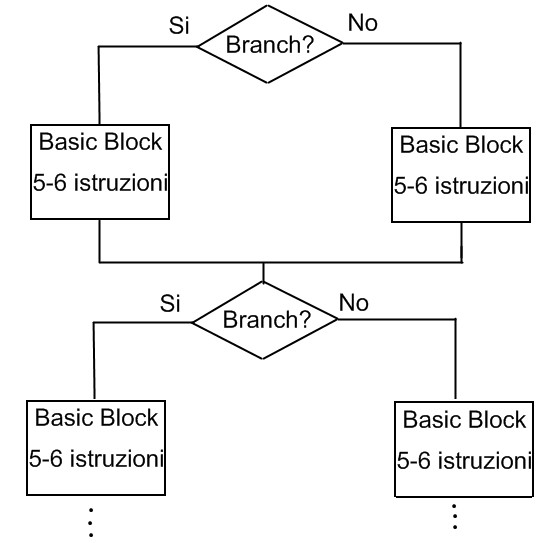
\includegraphics[width=0.5\columnwidth]{img/flowChartTipo}
\caption{Tipica \textit{flow chart} di un programma}
\label{fig:flowChartTipo}
\end{figure}

Statisticamente si è appurato che, tra \textit{branch} e \textit{branch}, vi sono sempre circa 5-6 istruzioni indipendenti (vedi fig. \ref{fig:flowChartTipo}). Nell'esecuzione speculativa, quindi viene in genere eseguito almeno un BB (\textit{basic block}) successivo dopo una \textit{branch}, validando ciò che si è fatto una volta che si è scoperto di aver evitato l'alea oppure annullando tutto in caso di \textit{misprediction} (qui torna utile l'abilità della CPU di poter fermare la \textit{pipeline} in modo che tutte le istruzioni precedenti la \textit{branch} siano completate e senza che le istruzioni successive abbiano effetto).

\section{L'approccio di Tomasulo}
\label{sec:tomasulo}

L'algoritmo di Tomasulo è un approccio di \textit{scheduling} dinamico per l'esecuzione delle istruzioni:
\begin{itemize}
\item consente di riconoscere situazioni di ILP non riconoscibili al tempo di compilazione;
\item riduce la complessità dei compilatori;
\item consente al codice compilato per una \textit{pipeline} di essere eseguito anche su \textit{pipeline} diverse;
\item rende molto più complesso l'hardware dell'unità di esecuzione.
\end{itemize}

In base ad esso, ogni unità di esecuzione \textit{multicycle} viene equipaggiata con stazioni di prenotazione (\textit{reservation stations}) che ospitano sia l'istruzione in esecuzione, sia istruzioni pronte per essere eseguite e in attesa dell'unità di esecuzione, sia istruzioni sospese in attesa di uno o due
operandi. Nello stadio ID l'istruzione viene decodificata e inviata a una appropriata \textit{reservation
station}, se disponibile; altrimenti, causa alea strutturale o mancanza di
\textit{reservation stations}, si stalla. 

\begin{figure}[!h]
\centering
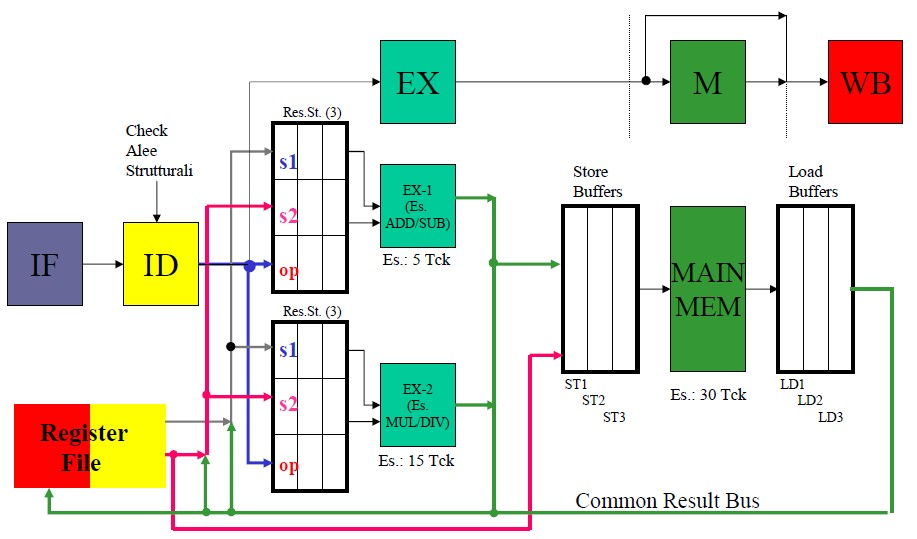
\includegraphics[width=0.9\columnwidth]{img/tomasulo}
\caption{Architettura prevista per il funzionamento dell'algoritmo di Tomasulo}
\label{fig:tomasulo}
\end{figure}

Alla \textit{reservation station} vengono inviati anche gli operandi, se disponibili; altrimenti si invia l'identificatore (\textit{tag}) della RS che fornirà l'operando mancante (nel caso dell'alea di dato). Il risultato generato dall'unità EX, insieme al \textit{tag} della RS che identifica l'operazione eseguita, viene messo a disposizione del \textit{register file} (in modo che possano usufruirne tutte le unità di EX che lo richiedono) e dello stadio MEM (attraverso il \textit{Common Result Bus}). Le alee RAW sono dunque risolte con il \textit{forwarding} (cioè l'invio) dei risultati a tutte le unità che hanno bisogno di operandi (\textit{reservation stations} e memorie).

\begin{figure}[!h]
\centering
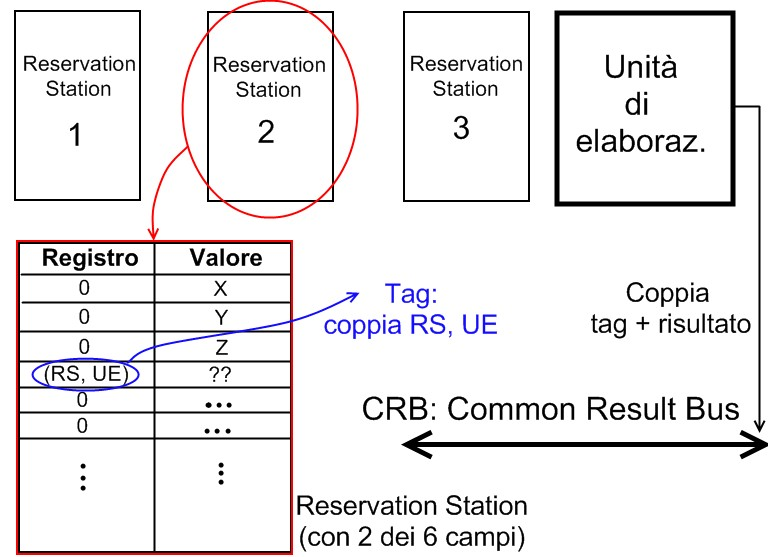
\includegraphics[width=0.75\columnwidth]{img/tomasulo2}
\caption{Architettura prevista per il funzionamento dell'algoritmo di Tomasulo (2)}
\label{fig:tomasulo2}
\end{figure}

Colui che ha bisogno di un risultato controllerà il CRB cercando in base al tag. Infatti, ad ogni unità che produce risultati (\textit{Load Buffer, Reservation Station}), è associato un identificatore che viaggerà sul \textit{Result Bus} insieme al risultato stesso.

Le \textit{reservation station} hanno 6 campi (in figura \ref{fig:tomasulo2} ne vengono illustrati solo 2):
\begin{itemize}
\item  BUSY: indica se la RS è libera o occupata
\item  $Q_j$ e $Q_k$: contengono l'identificatore del \textit{Load Buffer} o della \textit{Reservation
Station} che produrrà l'operando sorgente ($j$: 1° operando, $k$: 2° operando)
\item  $V_j$ e $V_k$: contengono l'operando se $Q_j$ / $Q_k$ = 0
\item  OP: operazione da eseguire (Es: FADD/FSUB\ldots)
\end{itemize}
\begin{figure}[!h]
\centering
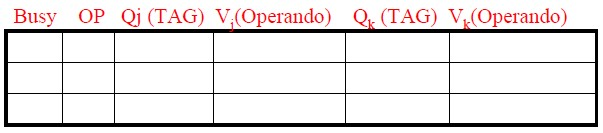
\includegraphics[width=0.75\columnwidth]{img/reservationStation}
\caption{I campi della \textit{reservation station}}
\label{fig:reservationStation}
\end{figure}

Poniamo ora di essere nella fase di ID (per ipotesi) di un'operazione DIV fra gli operandi OP1 e OP2. Abbiamo una \textit{reservation station} libera? Se sì la prenotiamo e, nel \textit{register file}, scriviamo la coppia (RS, UE): questo significa che il \textit{register file} aspetta il risultato dalla \textit{reservation station} RS appartenente all'unità operativa UE. Quando essa giunge alla fase di WB, viene scritto su CRB il risultato abbinato al relativo \textit{tag}: a quel punto il \textit{register file} si accorge che il risultato c'è è setta l'identificativo "'0'" (= dato disponibile, vedi campo \textit{registro} in fig. \ref{fig:tomasulo2}) presso il relativo operando. In questo modo deleghiamo la comunicazione del risultato alla \textit{reservation station}, utilizzando i \textit{tag} per suggerire cosa dovrà essere pescato dal \textit{common result bus}.

I registri posti prima del CRB (vedi fig. \ref{fig:tomasulo}) servono per evitare l'eventualità di due WB contemporanee (NOTA: la disponibilità di un operando si ha a partire dal termine della fase di WB): all'interno dello stesso ciclo di clock possiamo quindi scrivere più di un registro a monte del CRB, ma su quest'ultimo può essere scritto solo un dato alla volta.
Di conseguenza si ha che, con un solo CRB, non potremo effettuare più di un'operazione per clock ($CPI_{max} =1$); con più CRB è invece possibile completare più istruzioni simultaneamente (cioè in un singolo clock):
\[
N_{CRB} = N_{\text{Istruzioni simultaneamente completabili}}
\]
Nel caso di unico CRB e necessità di completare due istruzioni, è indifferente quale delle due scrivere per prima: negli esercizi si consiglia di scegliere una regola e agire coerentemente ad essa.

\section{Architettura protetta e Tomasulo}
\label{sec:protectedTomasulo}

Supponiamo di dover effettuare la seguente serie d'operazioni:
\begin{verbatim}
FDIV    F5, F1, F2
FADD    F20, F20, F21
FSUB    F5, F20, F12
\end{verbatim}
Se per caso F2 valesse zero avremmo un'operazione illegale (divisione per zero) e quindi verrebbe lanciata un'eccezione tramite un \textit{interrupt}, che fungerebbe da spartiacque fra le istruzioni precedenti e quelle successive. Se agissimo secondo una logica puramente sequenziale (\textit{In Order Issue}) saremmo costretti a stallare fino alla risoluzione dell'eccezione; se invece eseguissimo \textit{Out Of Order} dovremmo stare attenti a   non sporcare il valore dei registri completando istruzioni successive con operandi non aggiornati. Come abbiamo già detto, la politica è quella di salvare i risultati in un \textit{buffer} temporaneo e di farli diventare definitivi una volta che si è effettuato il controllo di \textit{safety}, cioè di sicurezza (correttezza). In effetti questa è una parte molto delicata per il funzionamento della nostra \textit{pipeline}: abbiamo accennato infatti alla possibilità di effettuare esecuzione speculativa, azzardando una predizione per un certo numero di istruzioni successive (dipendente dal numero di \textit{reservation station}), e abbiamo sottolineato l'importanza di poter annullare quanto supposto in caso di \textit{misprediction}. Quanto auspicato è ottenibile con Tomasulo se aggiungiamo una fase di \textit{Write Temporary} (WT, vedi fig. \ref{fig:safetyTomasulo}), durante la quale è il ROB (\textit{re-order buffer}, vedi fig. \ref{fig:safetyTomasulo2}) e non il \textit{register file} a mettere a disposizione i risultati.

\begin{figure}[!h]
\centering
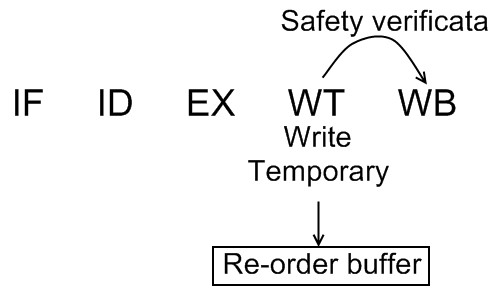
\includegraphics[width=0.5\columnwidth]{img/safetyTomasulo}
\caption{Miglioramento alla soluzione di Tomasulo}
\label{fig:safetyTomasulo}
\end{figure}

\begin{figure}[!h]
\centering
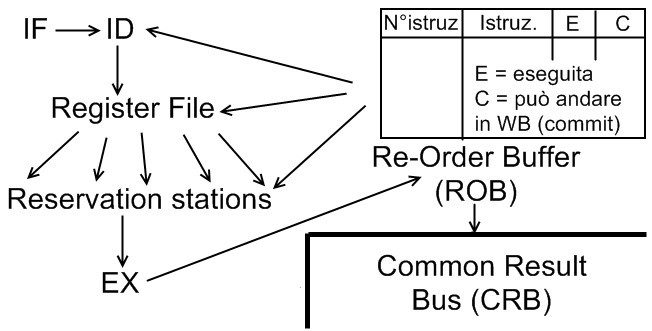
\includegraphics[width=0.65\columnwidth]{img/safetyTomasulo2}
\caption{Miglioramento alla soluzione di Tomasulo (2)}
\label{fig:safetyTomasulo2}
\end{figure}

Quando abbiamo predetto bene, nel ROB vengono posti degli 1 in prossimità delle istruzioni eseguite perché potevano effettivamente esserlo. Una volta che tale ambiguità è stata risolta, la parte completata viene svuotata dal ROB.
Pertanto, in questo nuova logica, il TAG non è più (RS, UE) ma l'indice nel ROB in cui è posta l'istruzione che deve restituirci il risultato.

Questo sistema è robustissimo con le alee RAW e, abbinato a una robusta logica di predizione (per evitare le alee di controllo in particolare), garantisce un'ottima protezione. 

\section{Protezione e memorie associative}
\label{sec:memorieAssociative}

Il problema dell'esecuzione speculativa richiede una nuova struttura dati per memorizzare i PC relativi ad una scelta di predizione rispetto che ad un altra (vedi fig. \ref{fig:plusFour}): una scelta funzionale e in grado di garantire velocità e affidabilità è quella che vede l'utilizzazione di una memoria associativa (nome/valore, detta CAM - \textit{Content Access Memory}).

\begin{figure}[!h]
\centering
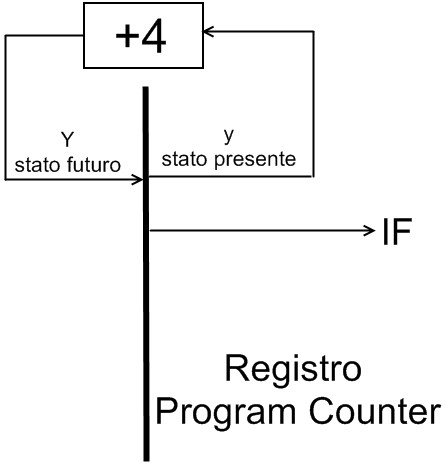
\includegraphics[width=0.35\columnwidth]{img/plusFour}
\caption{Usuale calcolo del PC: come ci regoliamo nel caso di predizione di salto?}
\label{fig:plusFour}
\end{figure}

Ogni volta che si abbisogna di un dato si controlla ispezionando la colonna \textit{nome} della nostra memoria: se trovo l'informazione cercata ho una \textit{hit}, altrimenti una \textit{miss}.
Volendo costruire questo tipo di memoria affinché sia superveloce bisogna inserire un comparatore per ogni elemento della tabella, in modo da confrontare il nome cercato con tutte le possibili \textit{entry} (memoria \textit{fully associative)}: facendo l'OR logico di tutte le uscite dei comparatori (1 = presenza, 0 = assenza) siamo in grado di ottenere in segnale di MISS negato (o di HIT). Con questa scelta bastano pochissimi clock\footnote{Almeno uno, ma non tanti di più!} e la velocità è nettamente superiore a quella che si ha con un \textit{loop} software.

\begin{figure}[!h]
\centering
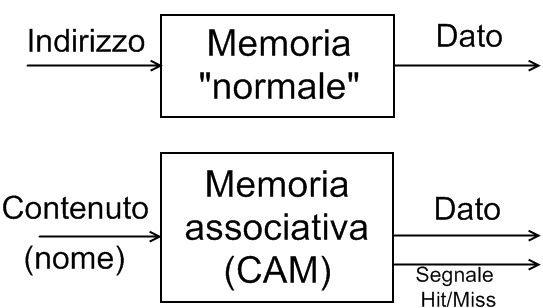
\includegraphics[width=0.4\columnwidth]{img/memVScam}
\caption{Memorie associative e memorie ordinarie (RAM, \textit{Random Access Memory})}
\label{fig:memVScam}
\end{figure}

A questo punto basta memorizzare, come coppie nome/valore, i PC futuri (cioè predetti) assieme al loro identificatore ed ecco che abbiamo ottenuto una velocissima struttura di predizione.
Grazie all'apparato di figura \ref{fig:plusFourModified} siamo quindi in grado di saltare, in base ad una corretta (\textit{hit}) o errata (\textit{miss}) predizione, al PC corretto. Il multiplexer in figura è un multiplexer a 32 bit e 2 vie (realizzato con 32 multiplexer da 1 bit).

\begin{figure}[!h]
\centering
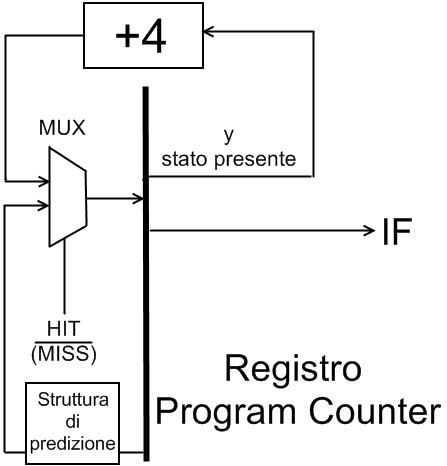
\includegraphics[width=0.4\columnwidth]{img/plusFourModified}
\caption{Versione modificata dell'apparato di selezione del PC}
\label{fig:plusFourModified}
\end{figure}

Come viene aggiornata la tabella? Il programma, quando scopre l'esistenza di una \textit{branch}, inserisce nella tabella il PC al quale si potrà saltare (se il salto avverrà) definisce una coppia nome/valore. La tabella (memoria associativa) verrà quindi esaminata ogniqualvolta si presenterà un'istruzione di salto: se sarà la prima volta che si effettua tale istruzione\footnote{CAM vuota: si cerca comunque di fare una predizione statica, non potendo fare diversamente.}, avremo obbligatoriamente una \textit{miss} e inseriremo il PC a cui si sarebbe dovuti saltare all'interno della CAM. Le volte successive, invece, saremo più fortunati se in tabella sarà ancora presente la \textit{entry} relativa a quel tipo di salto (cosa che molto plausibile che avvenga, vista l'esistenza del cosiddetto \textit{principio di località temporale}, il quale in soldoni recita che, effettuando spesso una certa istruzione o attingendo spesso a un dato, è molto probabile una futura intensa riutilizzazione di quell'istruzione/dato\footnote{"'Se faccio una cosa la riferò, se smetto di farla non la farò presumibilmente più'". (cit.)} in tempi relativamente brevi\footnote{Si pensi, ad esempio, ad un loop.}).

\section{Memorie associative e traduzione degli indirizzi}
\label{sec:associativeIndirizzi}

La CAM (che, organizzata come descritto, è detta anche \textit{Branch Tagged Buffer}) "'accelera la CPU'" conservando al suo interno i PC futuri che andranno quasi-sicuramente bene se vige il regime di località temporale (come effettivamente accade).
Nel caso la tabella sia piena o parzialmente piena, la cosa più logica è quella di cancellare l'istruzione non usata da più tempo: a far questo ci pensa un particolare algoritmo di sostituzione facente uso di una lista, detta \textit{list recently used}, in grado di discriminare le informazioni accedute più di recente. Inoltre, si cerca di mantenere gelosamente in tabella le istruzioni con il più basso parametro di \textit{miss-rate}\footnote{Calcolato come rapporta fra numero di \textit{miss} e numero di accessi.} (o il più alto \textit{hit-rate}), sacrificando piuttosto quelle con un più alto numero di \textit{miss}.

Questa tecnica viene utilizzata anche per la traduzione degli indirizzi delle istruzioni in \textit{cache} (indirizzati con 15 bit\footnote{Supponendo che la \textit{cache} sia di 32 KB.}) e quelle in memoria centrale (indirizzate con 32 bit\footnote{Supponendo che la memoria centrale sia di 4 GB.}). 
\[
IF_{32} \Rightarrow IC_{15}
\]
Stessa cosa può essere fatta tra memoria centrale e memoria virtuale\footnote{In informatica, la memoria virtuale è un tipo di memoria che ha la stessa funzione della RAM, ma viene usata solo se quest'ultima è piena e non riesce più a contenere informazioni; questo risultato si raggiunge utilizzando spazio di memoria secondaria su altri dispositivi, di solito le unità a disco (purtroppo più lente). La memoria centrale fisicamente presente diventa quindi la parte effettivamente utilizzata di quella virtuale, più grande: questo stratagemma è utile in virtù del principio di località e riuso dell'esecuzione dei programmi.}

\section{\textit{Pipeline} e linguaggi \textit{memory-register}}
\label{sec:pipelineMemoryRegister}

Quasi tutti gli esempi fatti fin'ora fanno riferimento alla struttura del DLX (registro-registro): come viene però implementata la \textit{pipeline} nei sistemi memoria-registro, con particolare riferimento al calcolo degli indirizzi (il quale dev'essere effettuato in maniera assolutamente trasparente)?

Per esemplificare consideriamo un linguaggio di tipo Intel e l'istruzione:
\begin{verbatim}
ADD     DS:[BX+DI], ALFA, AL
\end{verbatim}
L'indirizzo logico dell'operando sul quale andiamo ad agire è costituito dal binomio (base, offset) = $(DS, BX + DI + ALFA)$.
L'indirizzo fisico sarà invece pari a: $DS \cdot 2^4 + BX + DI + ALFA$ (dove il $2^4$ è dovuto al fatto che l'indirizzo in DS [\textit{Data Segment}] ha i quattro bit meno significativi sempre posti a 0 in quanto indirizziamo blocchi di $2^4$ byte sulla memoria fisica di 1 MB).
Dunque il calcolo dell'indirizzo fisico richiede di effettuare tre somme, terminate le quali l'indirizzo viene schiaffato\footnote{Termine tecnico.} sul bus degli indirizzi ($BA19,\ldots,BA0$).

Come effettuare queste operazioni in una \textit{pipeline}? Una prima modifica alla \textit{pipeline} che conosciamo, consiste nell'introduzione di un nuovo stadio a valle di ID destinato a calcolare l'indirizzo dell'operando in memoria (AG,\textit{ Address Generator}, o ID2, nome adottato da Intel per il Pentium): a tal fine lo stadio AG deve disporre di tre sommatori veloci in cascata.
Una seconda modifica consiste nel riunire i due stadi EX e MEM in un unico stadio (multiciclo) in cui sono localizzate la ALU e la cache dei dati. Questo stadio detto EX-MEM imporrà alle istruzioni la permanenza di un numero di colpi di clock variabile in funzione dell'istruzione eseguita: la valutazione viene effettuata considerando quante operazioni elementari di ALU o di accesso alla memoria devono essere effettuate per eseguire correttamente l'istruzione considerata\footnote{Esempi:
\begin{itemize}
\item  le istruzioni di trasferimento dati (con \textit{hit} in \textit{cache} dati) restano in EX-MEM un
periodo di clock;
\item  le istruzioni di ALU con un operando in memoria (\textit{hit}) e risultato su registro restano in
EX-MEM due clock (uno per leggere l'operando e uno per calcolare il risultato;
\item le istruzioni di ALU con un operando in memoria (\textit{hit}) e risultato in memoria restano
in EX-MEM tre clock (uno per leggere l'operando, uno per calcolare il risultato e uno
per aggiornare la memoria).
\end{itemize}
}

\begin{figure}[!h]
\centering
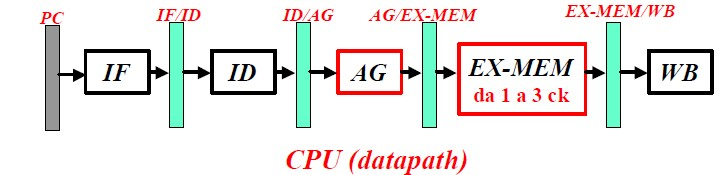
\includegraphics[width=0.8\columnwidth]{img/intelDataPath}
\caption{Modifiche alla \textit{pipeline} per sistemi Intel}
\label{fig:intelDataPath}
\end{figure}

Rispetto al DLX le cose vanno leggermente meglio grazie alla migliore densità del codice (il linguaggio Intel è CISC): il tutto mantenendo un CPI medio piuttosto piccolo (caratteristica dei sistemi RISC).


Come ci comportiamo con le istruzioni come quelle di \textit{push all}, in cui è necessario tradurre un'unica istruzione di linguaggio-macchina in almeno una decina di istruzioni elementari? La scelta effettuata è quella di bloccare la \textit{fetch} mentre viene alimentata la \textit{pipeline} con istruzioni elementari.

\subsection{Architetture superscalari}
\label{sec:superscalarArchitectures}

\begin{figure}[!h]
\centering
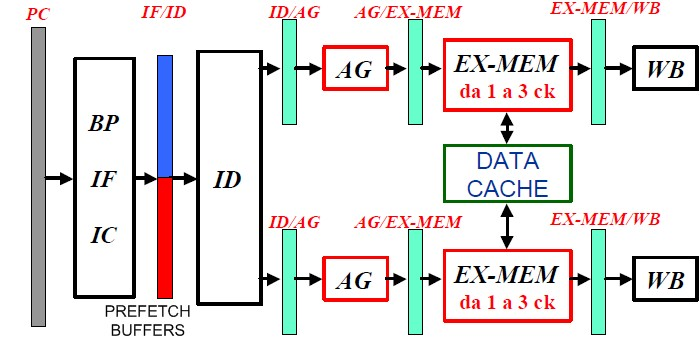
\includegraphics[width=0.9\columnwidth]{img/superscalare}
\caption{Schema di un'architettura superscalare (Pentium)}
\label{fig:superscalare}
\end{figure}

E se volessimo avere un parametro IPC (\textit{Instructions Per Clock} $= 1/CPI$) maggiore di 1? Dobbiamo ricorrere ad architetture cosiddette \textit{superscalari} (ad es. \textit{Pentium} IA32): si definisce infatti \textit{superscalare} una architettura che può attivare più di una istruzione nello stesso periodo di clock.
Nelle architetture superscalari lo stadio IF preleva in parallelo da IC frammenti di codice di
lunghezza maggiore o uguale a due istruzioni [nel Pentium: blocchi di codice di dimensione costante (32 byte) passati a ID attraverso un \textit{prefetch buffer}]; nello stadio AG vengono calcolati gli indirizzi degli operandi in memoria: le istruzioni complesse (istruzioni CISC descritte con microcodice) sfruttano le due \textit{pipeline} per una maggiore velocità.

In caso di istruzioni di trasferimento del controllo l'indirizzo di \textit{fetch} viene generato
dalla logica di predizione (ad esempio grazie alle memorie associative); successivamente IF preleverà codice anche dall'indirizzo associato alla situazione di \textit{misprediction} e lo appoggerà sull'altro \textit{prefetch buffer} Le istruzioni da decodificare si prelevano dallo stesso \textit{prefetch buffer} finché non si
verifica un errore di predizione, che viene rilevato alla fine della \textit{pipeline}. In caso di errore di predizione le \textit{pipeline} vengono svuotate e cambia il \textit{prefetch buffer} da cui si preleva il codice da eseguire: il \textit{prefetch buffer} è quindi in grado di ridurre il numero di stalli in caso di \textit{misprediction}.

ID riconosce due istruzioni consecutive sul \textit{prefetch buffer}, verifica che le due istruzioni
possano essere eseguite in parallelo e in tal caso le passa allo stadio a valle insieme al
contenuto dei registri operandi delle istruzioni. Se le due istruzioni non possono essere eseguite in parallelo (\textit{pairing rules} non soddisfatte), allora viene passata a valle una sola istruzione. Dallo stadio AG in poi le istruzioni che si trovano in stadi omonimi avanzano nella \textit{pipeline} insieme; se una istruzione stalla, stallerà anche l'altra, e stallano anche tutte le istruzioni che si trovano negli stadi a monte (\textit{pipeline} \textit{bloccanti}), dunque le istruzioni non possono sorpassarsi nella \textit{pipeline} (esecuzione e
completamento \textit{in ordine}).

Infine, al fine di ridurre gli stalli ogni \textit{pipeline} dispone, in EX-MEM, di un buffer di scrittura su cui
depositare indirizzi e dati da inviare alla memoria in caso di \textit{miss} in scrittura.

\chapter{Intel Architecture 32 bit, alcuni aspetti}
\label{cha:ia32}

\section{Bus e prime problematiche con la gerarchia delle memorie}
\label{sec:busMemorie}

Osserviamo la figura \ref{fig:strutturaInternaBus}; notiamo la presenza di due BUS principali, uno per la memoria (bus dati) e uno per le periferiche (IOB), separati da un \textit{bridge} fungente da ponte: si noti che essi hanno dimensione diversa (uno è a 64 bit, l'altro è a 8 bit). Ogni bus trasferisce una quantità di informazioni pari alla propria capacità ad ogni ciclo di clock, tuttavia non è detto che un singolo colpo di clock sia sufficiente per trasportare un intero dato. Prendiamo in considerazione le cosiddette "'linee di cache'"\footnote{Come nel caso delle memorie a livelli gerarchici superiori, anche la cache è suddivisa in blocchi di uguale dimensione. Nel caso delle cache questi blocchi sono detti \textit{linee di cache}. Nel Pentium e nel P6 (bus dati da 64 bit) la dimensione di ogni linea di cache è di 32 byte ed è identificabile dai 27 bit BA[31..5] (base) dell'indirizzo fisico costituito da 32 bit (27 bit base + 5 bit offset).}, unità grandi 32 byte in cui quest'ultima memoria è suddivisa: dovendo essere trasportate dal bus dati, si necessiterà di quattro cicli di bus per completare un singolo trasferimento. 

\begin{figure}[!h]
\centering
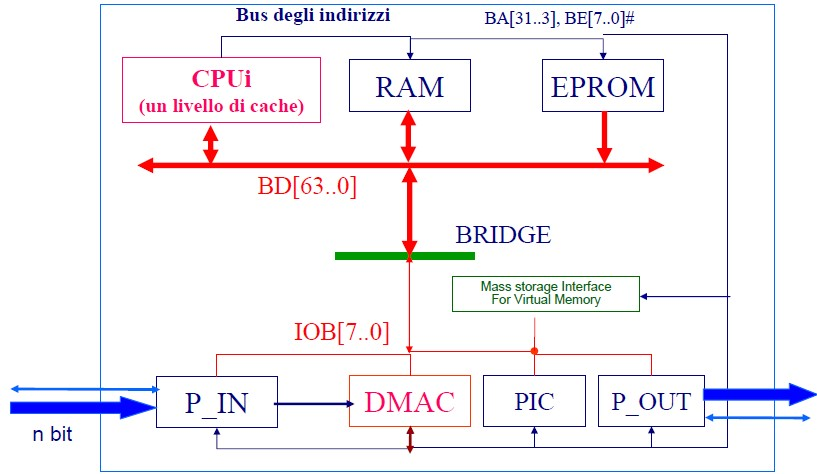
\includegraphics[width=0.85\columnwidth]{img/strutturaInternaBus}
\caption{Struttura interna della CPU}
\label{fig:strutturaInternaBus}
\end{figure}

Ogni ciclo di bus (dati), infatti, trasporta solo 8 dei 32 byte: da qui la necessità di effettuare cicli di bus multipli e di un segnale \textit{ready} (vedi fig. \ref{fig:segnaleReady}) in grado di indicare quando un dato è pronto e completamente trasferito. Inoltre, il meccanismo di generazione del segnale di \textit{ready} deve farci rispettare correttamente le tempistiche d'accesso alla memoria: se disponiamo, ad esempio, di una memoria con tempo d'accesso 100 ns e di un processore di 1 GHz dovremo aspettare 100 clock prima di poter effettuare le nostre operazioni.

\begin{figure}[!h]
\centering
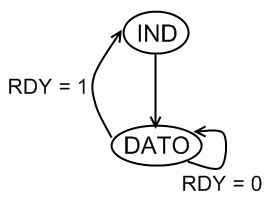
\includegraphics[width=0.35\columnwidth]{img/segnaleReady}
\caption{Funzionamento del segnale di \textit{ready}}
\label{fig:segnaleReady}
\end{figure}

Siamo quindi già arrivati a distinguere fra due diverse tipologie di cicli di bus:
\begin{itemize}
\item ciclo singolo: trasferiamo un unico dato;
\item ciclo \textit{burst}: trasferiamo quattro dati invece che uno solo (anche statisticamente si è visto che è la scelta migliore).
\end{itemize}
Purtroppo andare a leggere una periferica è un'operazione lentissima e abbiamo tempi d'accesso esorbitanti (confrontati con quelli d'accesso alla \textit{cache}); se il bus è bloccante ne segue che l'intera macchina lo è: volendo tuttavia poter usufruire dell'algoritmo di Tomasulo, il quale ci permette di eseguire fuori ordine, dobbiamo permettere che la memoria e l'I/O possano rispondere in ritardo (\textit{split transaction cycle}).

Inoltre, la CPU deve sapere a che ciclo di bus si riferisce un determinato dato: questo ci spinge ad inserire segnali di controllo e bit aggiuntivi. La cosa diventa ancora più complicata se abbiamo a che fare con sistemi \textit{multiprocessor}: dobbiamo infatti prevedere l'arbitraggio del bus, che è unico ed organizzato a mo' di \textit{pipeline} (cosicché serve dell'\textit{hardware} particolare per ogni stadio della pipeline e ulteriori segnali aggiuntivi... Non ne usciamo più!); infine possiamo avere in \textit{cache} delle copie di dati non consistenti (\textit{stail data}, dato presente in due memorie con valore diverso). Un analogo inconveniente può presentarsi per diversità dei dati fra la RAM e la \textit{cache} (problema di \textit{cache coherency}).
I componenti che si occupano di queste problematiche ed inoltre gestiscono le risorse, spegnendo la CPU in caso di emergenza o surriscaldamento, aumentando o riducendo la frequenza di \textit{clock}, etc\ldots sono i \textit{master} del bus (vedi fig. \ref{fig:busDintorni}.).

\begin{figure}[!h]
\centering
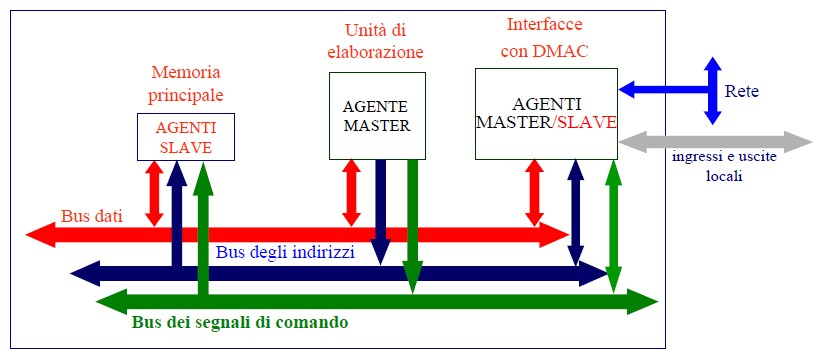
\includegraphics[width=0.75\columnwidth]{img/busDintorni}
\caption{Il bus e gli agenti interagenti con esso}
\label{fig:busDintorni}
\end{figure}

Morale della favola: un sistema complesso deve gestire moltissime cose e deve essere in grado di rilevare le occorrenze proibite, evitando che vengano eseguite e segnalando il \textit{software} con opportuni \textit{interrupt}\footnote{Prevenire è meglio che curare (cit.): serve obbligatoriamente un'opportuna \textit{routine} di gestione degli interrupt.}.

\section{IA32, protezione e gerarchia delle memorie}
\label{sec:gerarchia_memorie}

Osserviamo più da vicino al struttura del nostro processore Intel (vedi fig. \ref{fig:ia32}).

\begin{figure}[!h]
\centering
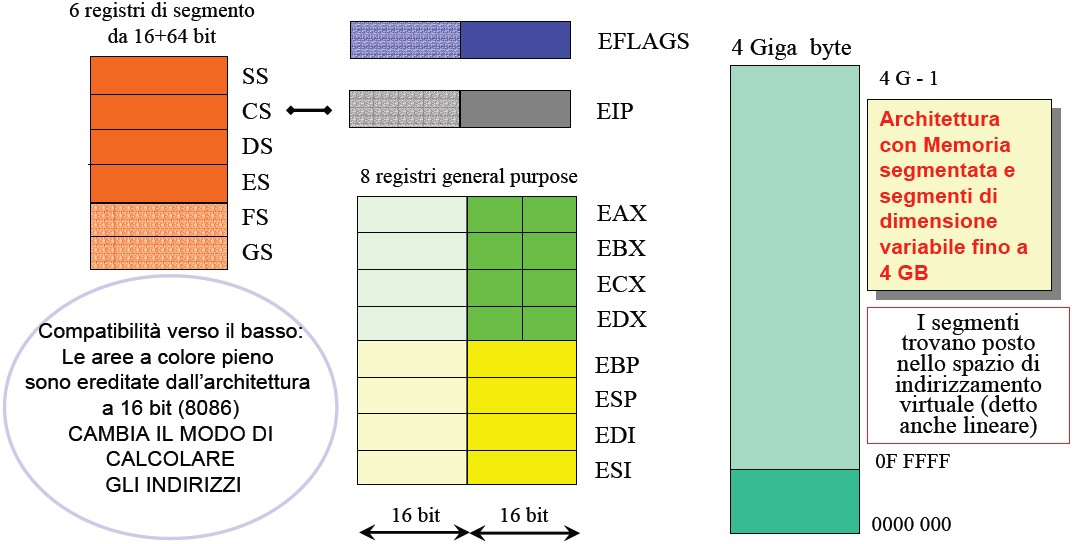
\includegraphics[width=\columnwidth]{img/IA32}
\caption{Ambiente di esecuzione di una applicazione
nell'architettura Intel a 32 bit.}
\label{fig:ia32}
\end{figure}

Qualche nota sui registri:
\begin{itemize}
\item ESP: \textit{Stack Pointer}. Si tratta dell'\textit{offset} nel registro di \textit{stack} dove siamo posizionati in un determinato momento;
\item EDI/ESI: registri indice per i vettori (max. 4 GB);
\item EIP: è l'\textit{Extended Instruction Pointer}, del quale presto scopriremo l'utilità;
\item sei registri di segmento entro i quali si manifesta la protezione\footnote{Una CPU protetta è una CPU in grado di separare i \textit{task} in base agli utenti che li hanno avviati.} della CPU (vedi capitolo \ref{cha:protezione}): essi indicano la tipologia, le proprietà, la dimensione e chi abbia il diritto d'accesso ad un certo segmento. Le CPU IA32 dispongono di sei registri di segmento: CS (\textit{code segment}: contiene il descrittore del blocco di codice in esecuzione), DS, ES, FS, GS ed SS (\textit{stack segment}: contiene il descrittore dello \textit{stack} in uso, v. paragrafo \ref{sec:controlliCPU}). La struttura di un registro di segmento è riportata in figura \ref{fig:regSegmento}.
\end{itemize}

Come nell'8086\footnote{Nell'8086 il \textit{Program Counter} era la coppia CS\#0000 + IP e puntava alla memoria di un 1 MB. Il PC era ottenuto da segmento + offset e si trovava in CS, con indirizzo iniziale FFFF0. In IA32, come si legge poco oltre, troviamo il descrittore di segmento, con indirizzo iniziale FFFFFFF0.}, per poter accedere a un segmento è necessario chi il relativo descrittore (per capire meglio cosa siano i descrittori si veda il paragrafo \ref{sec:descrittori}) sia stato preventivamente caricato in un registro di segmento. In particolare, CS contiene il segmento di codice del programma che in quel momento sta usando un'eventuale istruzione.

\begin{figure}[!h]
\centering
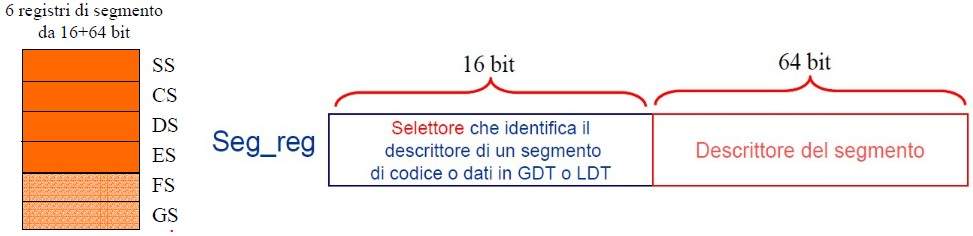
\includegraphics[width=0.84\columnwidth]{img/regSegmento}
\caption{Registro di segmento}
\label{fig:regSegmento}
\end{figure}

Nell'8086 ogni task ha 4 GB di memoria virtuale interamente dedicati a lui e sussistono sempre, anche se il quantitativo di RAM che ho nel sistema è molto inferiore: grazie a questo ingegnoso \textit{escamotage} siamo in grado di svincolare la dimensione del programma da quella della memoria fisica.

\begin{figure}[!h]
\centering
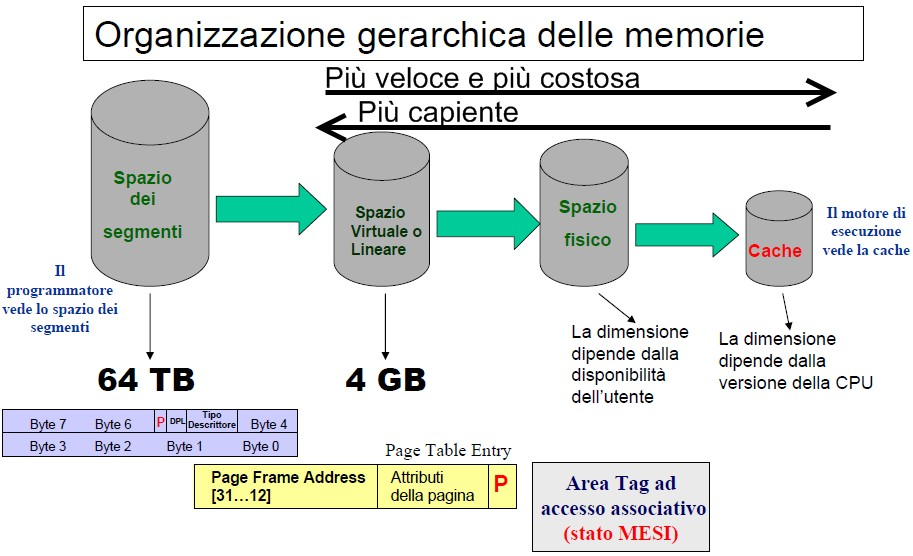
\includegraphics[width=\columnwidth]{img/slideSacra}
\caption{La gerarchia delle memorie}
\label{fig:slideSacra}
\end{figure}

A titolo informativo, mentre lo spazio dei segmenti e la \textit{cache} sono organizzati come matrici bidimensionali (a 2 coordinate), la memoria virtuale è lineare (1 coordinata).

Vediamo ora qualche esempio di codice in linguaggio macchina (NOTA: nei compiti segmento di codice, di dati e di \textit{stack} costituiscono un trinomio obbligatorio da definire!). \\
Segmento di \textbf{codice}:
\begin{verbatim}
             ER@10000H
Entry point: MOV DS, SEG_DATI
             ADD AL, DS:5 (aggiunge 5 ad AL)
             MOV DS: ALFA, AL 
             MOV EDI, 0 (mette a 0 EDI)
             MOV DS: BETA(EDI), EBX
             PUSH ...
             CALL ... (servirà supporto per il nesting!)
\end{verbatim}
Segmento \textbf{dati}:
\begin{verbatim}
         SEG_DATI SEGMENT RW@8000H (RW => leggere/scrivere)
8000H |  ALFA DB (DB => define byte)
8001H |  BETA DD 4DUP    (DD => double word = 4 byte)
...   |                  (4DUP => serve a duplicare 4 volte qualcosa)
      |                  (4 byte x 4 = 16 = 10H in esadecimale!)
8011H |  GAMMA DB
...
         ENDS
\end{verbatim}
Segmento di \textit{\textbf{stack}}:
\begin{verbatim}
STK_SEGMENT <..., ...>
\end{verbatim}

Notiamo che:
\begin{itemize}
\item la variabile ALFA è individuata dall'indirizzo logico <SEG\_DATI, 0>;
\item la variabile BETA(0) è individuata all'indirizzo logico <SEG\_DATI, 1>;
\item la variabile BETA(1) è individuata all'indirizzo logico <SEG\_DATI, 5>. Il 5 è stato calcolato ricordando che ogni elemento della struttura dati BETA è una \textit{double word} (4 byte);
\item gli indirizzi 8000H, 8001H, etc\ldots non sono indirizzi logici ma indirizzi nello spazio virtuale.
\end{itemize}

\begin{figure}[!h]
\centering
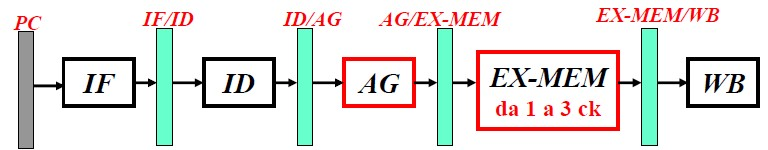
\includegraphics[width=0.8\columnwidth]{img/pipelineIndirizzi}
\caption{Pipeline e generazione degli indirizzi.}
\label{fig:pipelineIndirizzi}
\end{figure}

La pipeline come pensata in figura è in grado di funzionare su macchine M-R (come quelle Intel) e di effettuare la traduzione fra indirizzo logico e indirizzo virtuale. Ad esempio, ALFA ha indirizzo logico\footnote{Il programmatore (e i compilatori) vedono uno spazio di indirizzamento segmentato, il che significa che ogni istruzione e ogni dato vengono localizzati attraverso una coppia di coordinate: il segmento di appartenenza e la posizione (offset) all'interno del segmento (come in IA16); l'offset nel segmento può essere determinato dal compilatore (es. etichetta o variabile) oppure calcolato a \textit{runtime} (es. indirizzamento tramite registro base e registro indice).
} <SEG\_DATI, 0> ma indirizzo virtuale 8000H (+ offset pari a 0) calcolato facendo l'usuale operazione di somma base\footnote{DS concatenato con 4 zeri nell'8086; nell'IA32 è l'indirizzo virtuale calcolato nello stadio di AG, all'interno del quale è necessariamente utile avere i registri di segmento.} + offset.

\subsection{I \textit{Page Fault} e il reperimento dei blocchi}
\label{sec:pageFault}

Ogni volta che si esegue un \textit{task} è come se esistesse un file, all'interno dell'hard disk e grande 4 GB (ma magari "'scritto'" anche solo in pochi KB), che viene portato in memoria fisica (RAM): siccome la dimensione della RAM può essere anche molto inferiore a 4 GB, tale file viene smembrato in blocchi tutti uguali (pagine) di dimensione 4 KB. Se in memoria fisica viene ricercata una pagina che non c'è, allora si genera un \textit{page fault}, al quale si risponde caricando i dati cercati da memoria virtuale a memoria fisica.
La CPU, quando deve cercare qualcosa nella \textit{cache}, controlla i primi 27 bit dell'indirizzo fisico\footnote{Si ricorda che 27 dei 32 bit rappresentano la base e i 5 rimanenti l'offset.}.

\begin{figure}[!h]
\centering
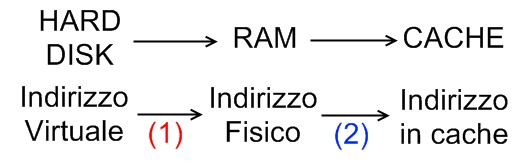
\includegraphics[width=0.6\columnwidth]{img/hdrc}
\caption{Indirizzi e rispettive locazioni}
\label{fig:hdrc}
\end{figure}

La traduzione degli indirizzi (vedi fig. \ref{fig:hdrc}) avviene attraverso tabella associativa (passaggio indicato col numero 1, IF-IC) oppure attraverso un \textit{Translation Look-Aside Buffer} (passaggio 2, IV-IF).
L'assenza di una pagina in memoria può avvenire ad ogni livello:
\begin{itemize}
\item \textit{page fault} (tra IV e IF);
\item \textit{miss} (tra IF e IC);
\item \textit{segment non present fault} (tra IL e IV).
\end{itemize}
Ovviamente l'architettura che gestisce tutte queste tipologie di \textit{miss} dev'essere adeguatamente veloce e deve sussistere una collaborazione HW-SW per gestire:
\begin{enumerate}
\item i \textit{cicli burst} per portare i dati in \textit{cache};
\item l'allocazione delle pagine in memoria centrale, attività della quale si occupa in genere il sistema operativo;
\item il reperimento delle informazioni non ancora presenti in memoria virtuale (\textit{segment non present fault});
\item il controllo sugli accessi in memoria (protezione);
\item la definizione di processi e delle risorse di memoria ad essi associati;
\item la separazione tra processi (protezione);
\item la commutazione tra un processo e l'altro (\textit{task switching});
\item le tecniche d'accesso all'hard disk, che è risaputamente un collo di bottiglia per le prestazioni.
\end{enumerate}
Tutto ciò (soprattutto i punti 1, 2, 3 e 8) è causa una gran mole di \textit{overhead}, ma fortunatamente il numero di \textit{miss} non è così grande grazie al principio di località.

\section{Descrittori di segmento}
\label{sec:descrittori}

Tutto quello che abbiamo detto sta in piedi se disponiamo di alcune informazioni importanti:
\begin{itemize}
\item a che livello è mappato il blocco di dati?
\item a che indirizzo?
\item quanto è grande?
\item è presente o devo trasferirlo?
\end{itemize}
Tutti questi particolari sono ben annotati nei cosiddetti \textit{descrittori}. Nell'architettura IA32 i descrittori hanno una struttura come indicato in figura \ref{fig:descrittoreGenerico}.

\begin{figure}[!h]
\centering
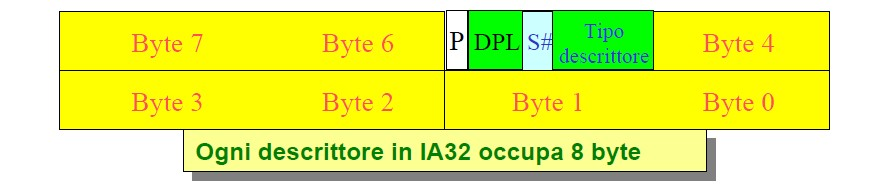
\includegraphics[width=0.75\columnwidth]{img/descrittoreGenerico}
\caption{Struttura generica di un descrittore}
\label{fig:descrittoreGenerico}
\end{figure}

Ad ogni segmento è associato un descrittore di 8 byte contenente tutti gli attributi del segmento (indirizzo di origine, lunghezza del segmento, diritti di accesso, tipo, etc\ldots). Per accedere a un oggetto in memoria è necessario conoscere il segmento di appartenenza; il relativo selettore deve essere caricato in un registro di segmento i quali sono sei\footnote{Quindi in ogni istante il programma ha la visibilità di non più di sei segmenti.}.

In IA32 la dimensione massima di un segmento è 4 GB; all'interno del descrittore sono contenute le informazioni necessarie per verificare se un accesso al segmento è lecito e in tal caso indica dove il segmento si trova.
Il linguaggio macchina delle CPU da 32 bit è un'estensione di quello dei processori 8086/88: così come questi due ultimi processori avevano una memoria segmentata, così anche per l'architettura a 32 bit ad ogni segmento è associato un \textit{descrittore di segmento} (vedi fig. \ref{fig:descrittoreSegDati}). Il descrittore va caricato in un registro di segmento, così come andava caricato in DS l'indirizzo iniziale del segmento in IA16\footnote{Data l'istruzione \textit{assembler} (ALFA è l'offset):\\
\texttt{MOV AL, ES:[ebx + edi].ALFA }\\
L'indirizzo virtuale è calcolato così:\\
\texttt{IV = ES.base\_seg + EBX + EDI + ALFA}\\
In generale, l'indirizzo virtuale (o lineare) di un operando in memoria in IA32 è infatti:\\
\texttt{IV = seg\_reg.base\_seg + EA}}.

\begin{figure}[!h]
\centering
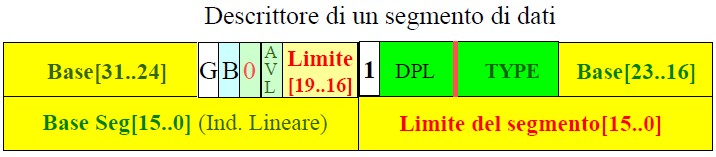
\includegraphics[width=0.75\columnwidth]{img/descrittoreSegDati}
\caption{Descrittore di un segmento dati}
\label{fig:descrittoreSegDati}
\end{figure}

In generale nell'architettura IA32 i descrittori vengono utilizzati non solo per descrivere e gestire i segmenti di codice e dati, ma anche per descrivere e gestire altri tipi di oggetti detti \textit{oggetti di sistema}\footnote{Il bit S\# definito nel byte 5 del descrittore consente di specificare se tale descrittore descrive un oggetto di sistema (S\# = 0) o un oggetto dell'applicazione (S\# = 1).
Gli oggetti dell'applicazione sono suddivisi in:
\begin{itemize}
\item segmenti di codice;
\item segmenti di dati e/o \textit{stack}.
\end{itemize}
Gli oggetti di sistema suddivisi in:
\begin{itemize}
\item segmenti contenenti i descrittori di task detti TSS o \textit{Task
State Segment};
\item porte di accesso a task e procedure di servizio dette \textit{Gates}
(i \textit{Gates} controllano sia l'accesso eseguito a controllo di
programma, sia l'accesso eseguito in risposta a eventi
interni o esterni);
\item tabelle con l'elenco degli oggetti accessibili a un task (\textit{Local
Descriptor Table} o LDT).
\end{itemize}
}

I descrittori sono radunati in apposite tabelle dette \textit{tabelle dei descrittori} (\textit{Global Descriptor Table}, GDT, \textit{Local Descriptor Table}, LDT), come illustrato in figura \ref{fig:sedeDescrittori}. È possibile accedere a un descrittore attraverso una chiave di accesso di 16 bit (detta selettore, la cui struttura è riportata in figura \ref{fig:strutturaSelettori}) contenente sia l'identificatore della tabella (GDT o LDT) sia l'indice del descrittore nella tabella (13 bit). Entrambe le tabelle contengono al massimo 8192 elementi di 8 byte.

\begin{figure}[!h]
\centering
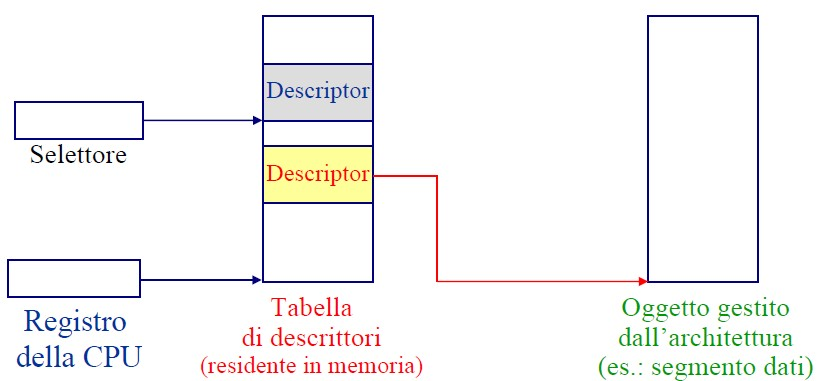
\includegraphics[width=0.75\columnwidth]{img/sedeDescrittori}
\caption{Locazione dei descrittori}
\label{fig:sedeDescrittori}
\end{figure}

\begin{figure}[!h]
\centering
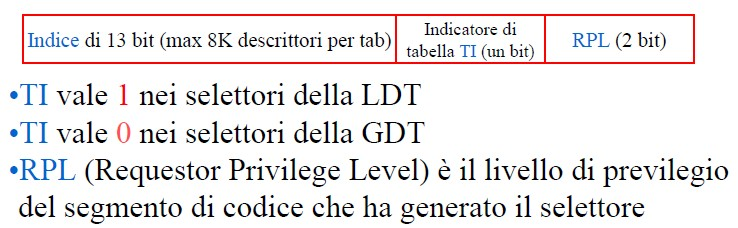
\includegraphics[width=0.75\columnwidth]{img/strutturaSelettori}
\caption{Struttura dei selettori}
\label{fig:strutturaSelettori}
\end{figure}

I descrittori sono parecchi: ve n'è un tipo per i segmenti di dati, uno per i segmenti di codice, uno per i \textit{task}, etc\ldots Per questo esiste anche un identificatore del tipo di descrittore: esso consta di 5 bit, dei quali solo 4 vengono in realtà usati (il primo è fisso ad 1), per un totale di 16 possibili oggetti all'interno della CPU.

\subsection{Descrittore di dato}
\label{sec:descrittoreDato}

\begin{figure}[!h]
\centering
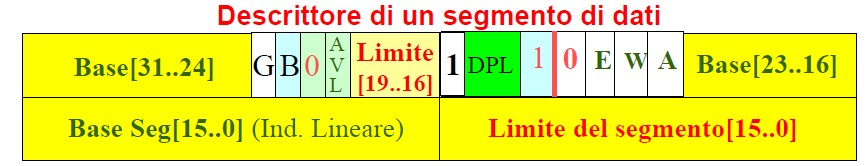
\includegraphics[width=0.75\columnwidth]{img/segDati}
\caption{Descrittore di dato}
\label{fig:segDati}
\end{figure}

In questo descrittore (vedi fig. \ref{fig:segDati}):
\begin{itemize}
\item DPL è il livello di privilegio del segmento associato al descrittore (\textit{Descriptor privilege level});
\item il bit più significativo del campo "'tipo descrittore'" discrimina tra segmenti di dato e segmenti di codice;
\item il bit A (\textit{Accessed}) è resettabile dal software e viene settato automaticamente ogni volta che viene fatto un accesso al segmento (cioè ogni volta che il descrittore viene caricato su un registro di segmento);
\item il bit E (\textit{ExpandDown}) definisce un segmento dati per il quale il limite è l'indirizzo più basso del segmento (segmento di \textit{stack} che cresce verso indirizzi decrescenti);
\item la base del segmento (per esempio l'indirizzo iniziale del segmento in uno spazio di indirizzamento lineare di 4GB) è memorizzato nei byte 2, 3, 4, 7 (vedi fig. \ref{fig:descrittoreGenerico}). Lo spazio di indirizzamento lineare può essere la memoria fisica o la memoria virtuale;
\item il limite del segmento è un campo di 20 bit memorizzato nei byte 0 e 1 e nei bit [0..3] del byte 6 (vedi fig. \ref{fig:descrittoreGenerico}); nei segmenti di codice e nei segmenti dati con E = 0 l'indirizzo base + limite è l'indirizzo lineare più alto del segmento associato al descrittore. Nei segmenti dati con E = 1, invece, sono vietati tutti gli accessi a indirizzi compresi tra base e base + limite;
\item anche se il campo limite è di 20 bit, la dimensione massima di un segmento non è limitata a un MB, ma può essere anche di 4 GB, infatti l'unità di misura di questo campo può essere il byte o la pagina di 4 KB; chi definisce l'unità di misura è il bit G (\textit{granularity});
\item bit G (\textit{Granularity}): se G = 0, il limite è espresso in byte; se G = 1 il limite è espresso in pagine di 4KB;
\item il bit B riguarda la gestione dei segmenti di \textit{stack}: se B = 1 lo \textit{stackpointer} è di 32 bit (ESP) e l'offset massimo è 0F FFFF FFFH, altrimenti lo \textit{stackpointer} è di 16 bit (SP) e l'offset massimo è 0F FFFH;
\item il bit AVL è un bit disponibile (\textit{available}) a chi scrive il sistema operativo;
\item il bit P (\textit{Present}, vedi fig. \ref{fig:regSegmento}, nella \ref{fig:segDati} è ad 1) indica se il segmento è mappato nel livello adiacente della gerarchia delle memorie (cioè se è mappato in memoria virtuale).
\end{itemize}


\subsection{Descrittore di codice}
\label{sec:descrittoreCodice}

\begin{figure}[!h]
\centering
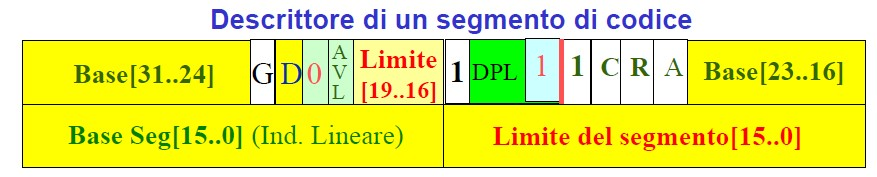
\includegraphics[width=0.75\columnwidth]{img/segCodice}
\caption{Descrittore di codice}
\label{fig:segCodice}
\end{figure}
Oltre ad alcuni attributi illustrati nel paragrafo \ref{sec:descrittoreDato}, abbiamo (vedi fig. \ref{fig:segCodice}).
\begin{itemize}
\item il bit W (\textit{Writable}) stabilisce se un segmento dati è di tipo \textit{Read/Write} o \textit{Read Only};
\item bit D nei segmenti di codice vale 1 se il codice è scritto nel linguaggio macchina della IA-32, mentre vale 0 se si tratta di codice macchina del processore 8086 (in particolare operandi e offset di 16 bit);
\item il bit R (\textit{Readable}) stabilisce se un segmento di codice è di tipo \textit{Execute/Read} o \textit{Execute Only}, cioè se contiene anche dati o è solo eseguibile;
\item il bit C (\textit{Conforming}) di un segmento di codice indica che il livello di privilegio a cui il segmento viene fatto eseguire è quello del codice che ha messo in esecuzione il segmento stesso (il segmento cioè eredita il livello di privilegio del codice chiamante).
\end{itemize}

Si ricorda che il descrittore di codice corrente è contenuto nel registro CS del nostro microprocessore.

\section{Politiche d'avvio e descrittori}
\label{sec:avvioDescrittori}

\begin{figure}[!h]
\centering
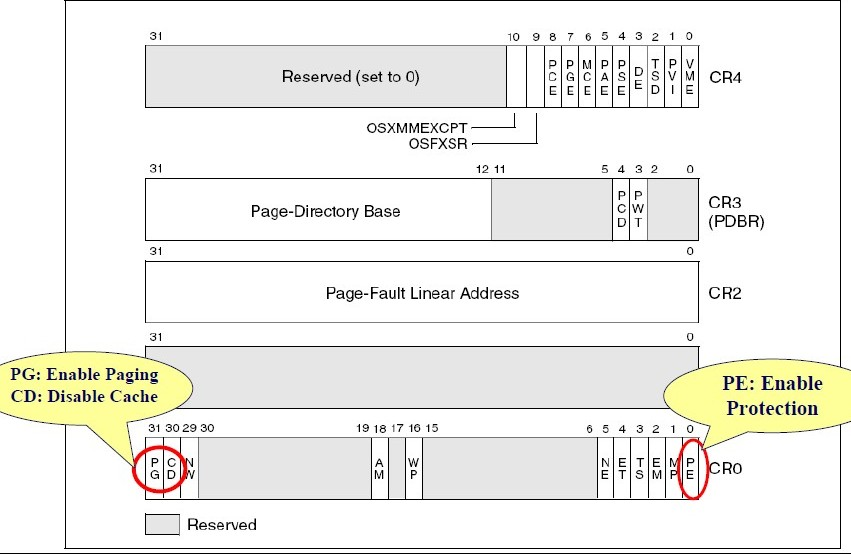
\includegraphics[width=0.9\columnwidth]{img/PGeRegistri}
\caption{I registri di controllo della CPU e l'abilitazione dei diversi livelli della gerarchia delle memorie}
\label{fig:PGeRegistri}
\end{figure}

La memoria, all'accensione della macchina, deve partire con i descrittori (e relative tabelle) già pronti: a tal proposito, le tabelle vanno portate nella memoria (vergine) non appena viene fatto partire il nostro dispositivo. Mentre però viene effettuato lo \textit{start-up}, la CPU si comporta come un 8088 (che non aveva i descrittori e quindi può benissimo funzionare senza!) e fa uso di un registro (CR0, vedi figura \ref{fig:PGeRegistri}) che si occupa di gestire il transitorio in cui non si ha alcuna tabella. Il bit PE (\textit{Protection Enable}) è pari a 0 durante tutta la transizione e va ad 1 quando finalmente tutto è pronto per funzionare a regime\footnote{Se PG=0 la memoria virtuale è disabilitata quindi l'indirizzo si riferisce alla memoria fisica. Se PG=1 la memoria virtuale è abilitata e gli indirizzi fanno riferimento alla memoria virtuale (in particolare il registro BASE SEG).}.

Mentre la CPU si accende, la \textit{cache} è disabilitata (CB=1) e anche l'impaginazione (PG=0) lo è: ufficialmente, sotto quest'ultimo punto di vista, tutto funziona come nell'IA16.
Abilitata \textit{cache} e impaginazione, dispongo della gerarchia completa delle memorie.

\section{Ciclo IDLE e considerazioni sui consumi}
\label{sec:idleConsumi}

Il ciclo \textit{idle} (vedi fig. \ref{fig:halt}) è attivo quando la CPU ha ben poco da fare: durante il suo svolgimento, la CPU va in HALT per cercare di spegnere quasi tutto e - di conseguenza - di consumare il meno possibile. I consumi di un moderno elaboratore possono infatti essere suddivisi in tre parti, più o meno equivalenti come dispendio:
\begin{itemize}
\item la CPU;
\item le periferiche (HD, monitor, etc\ldots);
\item tutto il resto (memorie, bridge, etc\ldots).
\end{itemize}

\begin{figure}[!h]
\centering
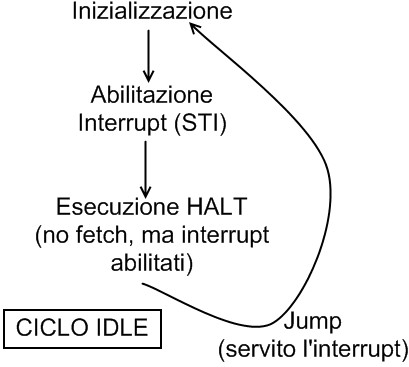
\includegraphics[width=0.55\columnwidth]{img/halt}
\caption{Struttura del ciclo \textit{idle}}
\label{fig:halt}
\end{figure}

Spegnendo la CPU abbatto i consumi di 1/3; altri accorgimenti per il risparmio dell'energia possono essere l'utilizzo della modalità \textit{standby}, lo spegnimento dell'\textit{hard-disk}, l'inibizione \textit{totale} del clock alla CPU o, infine, la riduzione della frequenza di funzionamento o della tensione\footnote{Servirà ovviamente un sistema di monitoraggio per decidere come modulare questi due parametri in base alla situazione.} in virtù della relazione
\[
P=KV^2f
\]
(con $K$ costante di proporzionalità, $V$ tensione e $f$ frequenza).

Ebbene, quando la CPU è in HALT viene generato un apposito ciclo di bus (che viene visto anche dal bridge) e che fa partire un \textit{timer} il quale, allo scadere, priva la CPU del clock.
Se togliamo anche l'alimentazione, la CPU passa in modalità \textit{deep sleep} (sonno profondo), in cui è il bridge a gestire gli \textit{interrupt}: il risveglio sarà lentissimo, ma almeno avremo risparmiato moltissima energia.


\chapter{Descrittori: protezione e interrupt}
\label{cha:protezione}

In generale una piattaforma \textit{multitasking} dispone di un sistema operativo (anch'esso composto da uno o più \textit{task}) che gestisce le risorse (rete, periferiche, \textit{file system}, etc.) per conto dei \textit{task} applicativi. I \textit{task} applicativi possono essere indipendenti tra loro e possono anche appartenere a utenti distinti: c'è pertanto la stringente esigenza di tenere separati i \textit{task} e soprattutto di evitare che un errore su un \textit{task} metta in crisi l'intera piattaforma. A tal fine l'architettura IA32 include meccanismi di protezione e separazione che si prefiggono i seguenti obiettivi: 
\begin{itemize}
\item impedire a un \textit{task} di modificare l'area dati di un altro \textit{task} (restrizione sulla visibilità della memoria)
\item impedire a un \textit{task} di accedere direttamente a una risorsa (es. periferica)
gestita dal sistema operativo (restrizione sull'input/output)
\item  in caso di errore in un \textit{task} non ben collaudato, assicurare la sopravvivenza del
sistema operativo e non compromettere la funzionalità degli altri \textit{task}
\end{itemize}
La restrizione di visibilità sulla memoria può essere effettuata come segue:
\begin{itemize}
\item  certi segmenti di dati (i.e. porzioni dello spazio di indirizzamento lineare)
possono essere associati solo a determinati \textit{task} e possono essere resi
invisibili ad altri;
\item a ogni \textit{task} può essere associato il proprio set di\textit{ page directory} e \textit{page tables};
in questo modo certe aree della memoria fisica possono essere rese accessibili
solo a determinati \textit{task} (e possono essere rese invisibili ad altri).
\end{itemize}

Per questo le strutture dati utilizzate dal software hanno livelli diversi di criticità\footnote{Ad esempio i descrittori dei \textit{task} e le\textit{ page table} sono più critici dei descrittori dei buffer di input/output, a loro volta più critici di una tabella di dati locale a una procedura utilizzata in un solo task applicativo.}
Risulta quindi opportuno introdurre un meccanismo che protegga i dati critici contro l'accesso da parte di codice non sufficientemente affidabile.

\section{Controlli della CPU}
\label{sec:controlliCPU}

Il linguaggio macchina della IA32 utilizza un modello di memoria segmentato come l'8086. Ogni riferimento a operandi in memoria o a istruzioni si compone di due coordinate: l'identificatore del segmento e l'offset. Tuttavia, mentre nell'8086 l'unica informazione specifica associata a un segmento era l'indirizzo iniziale (base del segmento), nella IA32 il descrittore del segmento, oltre alla base, contiene molte informazioni che consentono alla CPU di verificare la legittimità dell'accesso (architettura \emph{protetta}).

Ad ogni accesso a un segmento la CPU controlla quanto segue:
\begin{itemize}
\item se l'indirizzo appartiene effettivamente al segmento (check sul limite);
\item se il tipo di accesso è compatibile con il tipo del segmento (check sul tipo)\footnote{Ad esempio la CPU verifica se ogni operazione di \textit{fetch} è fatta su un segmento di codice oppure se una operazione di scrittura è indirizzata a un segmento di dati \textit{writable}.};
\item se i livelli di privilegio di codice e dati sono compatibili e se i livelli di privilegio di codice chiamante e codice chiamato sono compatibili (check sul dominio di indirizzabilità);
\item se l'istruzione in corso di esecuzione può legittimamente essere eseguita al livello di privilegio a cui sta eseguendo il \textit{task running}. Si definisce perciò il Livello di Privilegio Corrente (\textit{Current Privilege Level}, CPL) che in genere coincide col DPL (\textit{Descriptor priviledge level}), che è il livello di privilegio del segmento associato al descrittore di dato a cui accediamo in un determinato momento. Esistono quattro livelli di privilegio: Kernel (0, il più basso: il Kernel può fare tutto ciò che vuole!), Driver (1), \textit{File System} (2), Programma utente (3, il più alto). La CPU controlla dinamicamente la legittimità di ogni accesso a operandi in memoria confrontando i livelli di privilegio del codice in esecuzione con quello del segmento dati a cui deve accedere. Per fare sì che chi ha il controllo della CPU stia facendo qualcosa di legittimo, si controlla se il DPL del dato al quale si sta accedendo è \emph{Maggiore o uguale} al corrente livello di privilegio. In caso contrario viene restituito un errore di protezione.
\end{itemize}

Tutti questi controlli vengono eseguiti nella fase AG\footnote{Ricordiamo che si hanno le seguenti fasi: IF$\to$AD$\to$AG$\to$EX-MEM.} e, in caso di violazione di un livello di protezione, la CPU genera automaticamente una eccezione (\textit{General Protection Fault}).

\begin{figure}[!h]
\centering
\includegraphics[width=0.65\columnwidth]{img/livelliprivilegio}
\caption{Architettura protetta: livelli di privilegio}
\label{fig:livelliprivilegio}
\end{figure}

Un altro esempio di violazione si ha quando il sistema operativo "'sfora'" nello \textit{stack}: per questo esiste uno \textit{stack} per ogni livello di privilegio. Il descrittore dello \textit{stack} è contenuto nel segmento SS, come era già stato anticipato nel paragrafo \ref{sec:gerarchia_memorie}.

\section{\textit{Call gate}}
\label{sec:colgateDentifricio}

Supponiamo che, fra tutte le possibili \textit{system call} del nostro sistema solo alcune siano accessibili da noi poveri comuni mortali:
\begin{verbatim}
            LIVELLO di PRIVILEGIO
SYS 1       0
SYS 2       2, 1, 0
SYS 3       0
...         ...
SYS N       3
\end{verbatim}

\begin{figure}[!h]
\centering
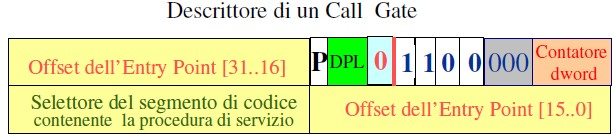
\includegraphics[width=0.65\columnwidth]{img/Callgate}
\caption{Descrittore di un \textit{call gate}}
\label{fig:Callgate}
\end{figure}

Le chiamate a procedura vengono fatte attraverso il \textit{call gate}, che è uno dei famosi "'oggetti di sistema'" noti alla CPU. Anche per i \textit{call gate} esiste un descrittore, in quanto è necessario sapere dove sia l'\textit{entry point} della procedura da chiamare, quali siano i dati per l'accesso, etc\ldots
Perché l'accesso ad una determinata procedura sia valido, si controlla che il livello di privilegio del chiamante sia maggiore o uguale a quello del chiamato. Ad ogni \textit{gate} viene infatti dato un certo livello di privilegio, così come si faceva coi segmenti di dati.

Quando accedo ad una \textit{call gate} (gestita come se fosse un segmento di dati), le istruzioni compiute dalla macchina sono quindi:
\begin{enumerate}
\item si guarda la struttura dalla \textit{call gate} e si prelevano i parametri necessari;
\item si aggiorna il registro CS con l'\textit{entry point};
\item si cambia lo \textit{stack}, sul quale viene salvato anche il puntatore al vecchio \textit{stack};
\item si portano i parametri nello \textit{stack} dedicato alla nostra procedura (tramite un contatore che ci aiuta  a prenderne il giusto numero misurato in \textit{double words}).
\end{enumerate}

\section{\textit{Interrupt gate, trap gate, task gate}}
\label{sec:interruptgate}

Si noti che anche il servizio di un \textit{interrupt}, formalmente, è una chiamata a procedura: nelle macchine Intel, perché esse siano eseguite, viene interpellato l'\textit{interrupt controller} (8254), il quale può gestire fino a 8 \textit{interrupt}.
Nell'8086/88 esiste una \textit{interrupt table} (vedi fig. \ref{fig:interruptTable}), presente all'indirizzo 0 e contenente gli indirizzi per le \textit{routines} di interrupt da servire. Ogni possibile \textit{interrupt} è identificato da 1 byte (per un totale di 256 possibili \textit{interrupt types}) il quale è emesso dal componente 8254 e ci fornisce la giusta chiave per passare alla routine di servizio.

\begin{figure}[!h]
\centering
\includegraphics[width=0.65\columnwidth]{img/interruptTable}
\caption{La \textit{Interrupt table}}
\label{fig:interruptTable}
\end{figure}

\begin{figure}[!h]
\centering
\includegraphics[width=0.75\columnwidth]{img/trasferimentoInterrupt}
\caption{Il meccanismo di trasferimento del controllo alle procedure di servizio dell'\textit{interrupt}}
\label{fig:trasferimentoInterrupt}
\end{figure}

Nell'8086 a partire dall'\textit{interrupt type} eravamo già in grado di ottenere il puntatore alla relativa procedura\footnote{La procedura di servizio dell'\textit{interrupt} farà sempre parte di un segmento di codice, il cui selettore dovrà pertanto essere contenuto nell'\textit{interrupt gate}. La procedura di servizio partirà infatti necessariamente da un certo offset nel suo segmento di codice, il quale dovrà pertanto essere contenuto nell'\textit{interrupt gate}.}. L'\textit{interrupt type} è infatti indice in una tabella che contiene i puntatori agli \textit{entry points} delle procedure di servizio degli \textit{interrupt} (dette anche \textit{continuators}). In un'architettura protetta (IA32) e \textit{multitasking}, invece, dobbiamo dare il puntatore all'\textit{interrupt gate}\footnote{Come distinguiamo un \textit{interrupt gate} da un \textit{task gate}?
\begin{itemize}
\item Se di tipo \textit{interrupt}: identificativo del descrittore = 01110 (E);
\item se di tipo \textit{task}: identificativo del descrittore = 00101 (5).
\end{itemize}
}, descrittore di sistema all'interno dei quali è codificato l'\textit{entry point} della procedura di servizio dell'\textit{interrupt}.

In IA32, queste entità si trovano in una tabella detta \textit{Interrupt Descriptor Table }(IDT, rimpiazzante la tabella IT dell'8086/88) il cui indirizzo lineare iniziale può essere cambiato dal software in quanto viene mantenuto in un apposito registro della CPU detto IDTR.

Quando serviamo un \textit{interrupt}, questi vengono disabilitati e infine riabilitati (IRET) una volta servito il nostro \textit{interrupt}. Se gli \textit{interrupt} sono disabilitati e dobbiamo gestirne degli altri, \emph{annidati}, questo meccanismo non funziona: dobbiamo altresì accoglierli e decidere in base alla priorità degli stessi (esaminata dall'\textit{interrupt controller}). Per questo esiste un modo di servire gli \textit{interrupt}, lasciandoli però abilitati: si fa uso dei \textit{trap gate}.

\begin{figure}[!h]
\centering
\includegraphics[width=0.65\columnwidth]{img/TrapGate}
\caption{Descrittore del \textit{trap gate}}
\label{fig:TrapGate}
\end{figure}

\begin{figure}[!h]
\centering
\includegraphics[width=0.65\columnwidth]{img/intTaskGate}
\caption{Descrittore di \textit{task gate} e \textit{interrupt gate}}
\label{fig:intTaskGate}
\end{figure}

La sequenza di procedure nel servire un \textit{interrupt} è quindi la seguente (vedi fig. \ref{fig:percorso}):
\begin{enumerate}
\item arriva un \textit{interrupt};
\item si consulta la IDT;
\item troviamo un \textit{trap gate} relativo alla \textit{routine} di interrupt da gestire;
\item andiamo a pescare il selettore nella GDT;
\item nella GDT sono presenti i descrittori dei TSS di ogni \textit{task};
\item ora che abbiamo il nostro TSS sappiamo quali pagine sono associate al nostro \textit{task} (abbiamo anche i puntatori alla \textit{Page Table} e alla \textit{Page Directory}). Inoltre, abbiamo a disposizione il selettore del descrittore della LDT associata al task;
\item tramite questo selettore accediamo nuovamente alla GDT, dove troviamo il descrittore della LDT;
\item ora finalmente sappiamo dov'è locata la \textit{Local Descriptor Table} e abbiamo così tutto ciò che ci serve per gestire l'\textit{interrupt};
\item finalmente effettuiamo la routine di servizio.
\end{enumerate}

\begin{figure}[!h]
\centering
\includegraphics[width=0.93\columnwidth]{img/percorso}
\caption{Percorso di servizio \textit{interrupt}}
\label{fig:percorso}
\end{figure}

\section{\textit{Task call e Task State Segment}}
\label{sec:taskGate}

\begin{figure}[!h]
\centering
\includegraphics[width=\columnwidth]{img/TSS}
\caption{\textit{Task State Segment}}
\label{fig:TSS}
\end{figure}

Il calcolatore dev'essere naturalmente in grado di gestire molti eventi al secondo, ma ha un unico \textit{program counter} (PC = CS:EIP) il quale dev'essere immediatamente aggiornato nel caso sopraggiungano nuovi elementi da servire: il processo per il quale il processore passa da un compito all'altro è chiamato \textit{context switching} (o \textit{task switching}). Nella nostra macchina possono essere attivi diversi \textit{task}, ognuno con un proprio stato e uno \textit{stack} dove andare a mettere i parametri. Le informazioni riguardanti ogni preciso \textit{task} si trovano nel descrittore del TSS (\textit{Task State Segment}), il quale è un segmento dati con una struttura e dei contenuti ben conosciuti e interpretabili dalla CPU\footnote{Oltre alle informazioni a cui si fa riferimento poco più avanti, il TSS della IA-32 contiene anche le seguenti informazioni
statiche (cioè definite al momento della creazione del task ed eventualmente modificate
dal SO):
\begin{itemize}
\item i selettori dei sei registri di segmento;
\item il valore degli 8 registri di uso generale (EDI, ESI, EBP, ESP, EBX,
EDX, ECX, EAX);
\item il valore del \textit{flag register} EFLAGS;
\item il valore dell'\textit{Instruction Pointer} EIP;
\item il selettore della LDT del \textit{task};
\item il contenuto del registro PDBR col puntatore all'indirizzo fisico della \textit{Page Directory} associata al \textit{task};
\item l'indirizzo logico (selettore e offset) degli \textit{stack} associati al \textit{task} (uno \textit{stack}
per ciascuno dei livelli di privilegio 0, 1 e 2);
\item un bit utilizzato in fase di \textit{debugging};
\item un'area di memoria opzionale a disposizione del sistema operativo(\textit{software state});
\item la mappa dei diritti di accesso alle interfacce di input/output.
\end{itemize}}. Il TSS contiene i riferimenti a codice, dati (registri GS, FS, DS, etc\ldots Essi sono copiati automaticamente nei registri dell'architettura quando si ha l'inizializzazione del \textit{task}) e \textit{stack} di ogni \textit{task}. Tali riferimenti vengono aggiornati ad ogni sospensione e consentono al \textit{task} di ripartire correttamente al momento della successiva messa in esecuzione. Inoltre, come si vede dalla figura \ref{fig:TSS}, il TSS contiene i riferimenti agli \textit{stack} associati ai livelli di privilegio\footnote{Tali riferimenti servono ogni volta che cambia il livello di privilegio del codice in esecuzione (PL decrescente).} da 0 a 2. Infine, il TSS contiene i campi LDT e CR3: il primo è il selettore del descrittore della \textit{Local Descriptor Table} del task, mentre il secondo è il riferimento alle pagine in memoria fisica in cui viene salvata la funzione che trasforma gli indirizzi virtuali del \textit{task} in indirizzi fisici. 
Come dicevamo, ogni TSS ha un descrittore, il quale può risiedere solamente nella GDT.

\begin{figure}[!h]
\centering
\includegraphics[width=0.65\columnwidth]{img/taskStateSegment}
\caption{Descrittore di un \textit{Task State Segment}}
\label{fig:taskStateSegment}
\end{figure}

In riferimento alla figura \ref{fig:taskStateSegment}, il significato dei campi \textit{Base}, \textit{Limite} e G è analogo a quello dei descrittori di segmenti di codice e dati. Il bit B (\textit{Busy}) vale 1 se il \textit{task} è \textit{running} (cioè in esecuzione) o è \textit{ready} (cioè in attesa di una CPU libera che lo possa mettere in esecuzione); se il bit B vale 0, allora il task è \textit{waiting}, cioè in attesa di un evento che lo attivi (vedi figura \ref{fig:taskStati}). Il tentativo di attivare un \textit{task} che è già attivo (bit B = 1) provoca una eccezione (task non \textit{rientranti}), mentre si può eseguire una seconda istanza di un \textit{task} definendo un secondo \textit{task} associato allo stesso codice. 

\begin{figure}[!h]
\centering
\includegraphics[width=0.55\columnwidth]{img/taskStati}
\caption{Possibili stati di un \textit{task}: \textit{running, ready, waiting}}
\label{fig:taskStati}
\end{figure}

Un \textit{task} può essere attivato non solo in seguito ad un evento, bensì anche in conseguenza della chiamata da parte di un altro \textit{task} (\textit{task call}); alternativamente, si può effettuare una chiamata a \textit{task} simultanea alla terminazione di un altro \textit{task} (istruzione \textit{Jump Task}).
Questo porta alla generazione una catena dinamica in cui ogni \textit{task} punta ad un processo più a valle (cioè a quello che l'ha chiamato), mentre quello più a monte è \textit{running} (vedi fig. \ref{fig:catenaTask}).

\begin{figure}[!h]
\centering
\includegraphics[width=0.65\columnwidth]{img/catenaTask}
\caption{Catena di \textit{task} dinamicamente costruita}
\label{fig:catenaTask}
\end{figure}

Il \textit{Task Register} (TR) è il registro che contiene l'ID del \textit{task} attualmente in \textit{running} (punta al TSS di quest'ultimo): quando un \textit{task} termina o si interrompe e un altro prende il suo posto basta quindi aggiornare il \textit{task register} per effettuare lo scambio. Se ora guardiamo nuovamente il  \textit{task state segment} (figura \ref{fig:TSS}) notiamo la presenza di un campo \textit{link}, puntante al \textit{task} immediatamente più a valle nella catena sopraccitata; se il \textit{task} più a valle della catena ha il campo \textit{link} = 0, non può terminare (non ha nessuno in coda) quindi diventa il \textit{task} IDLE con, come ultima istruzione, HALT.

Si dice anche che i \textit{task} possono essere annidati \textit{nested} (\textit{flag} NT): ovviamente l'ultimo \textit{task}, quello più in coda, ha NT = 0 visto che gli unici \textit{task} in grado di terminare sono quelli più a monte (\textit{nested}).

\begin{figure}[!h]
\centering
\includegraphics[width=0.59\columnwidth]{img/taskNonRientranti}
\caption{}
\label{fig:taskNonRientranti}
\end{figure}

Ora possiamo meglio capire cosa intendevamo per \textit{task non rientranti}; esaminiamo ad esempio la figura \ref{fig:taskNonRientranti}: la situazione in essa illustrata è illegale in quanto non si può chiamare un \textit{task} che è presente in coda (e, quindi, in stato \textit{ready}). Anche in questo caso il processore riuscirà ad evitare questa eventualità facendo uso del descrittore del TSS.

\section{Sistemi \textit{multiprocessor} e \textit{task}}
\label{sec:multiprocessorTask}

Nel caso di sistemi \textit{multiprocessor} si hanno più \textit{program counter} e, finché ci sono CPU libere, i \textit{task} permangono in \textit{running}. Chiaramente un'architettura così deve poter disporre di una \textit{cache} separata per ogni processore, in modo da sfruttare correttamente il parallelismo: sarebbe demenziale pensare di disporre di più processori ma dover condividere un'unica memoria fisica contendendosi il bus! I processori non potrebbero infatti lavorare contemporaneamente, eventualità auspicabile e che accade davvero nel caso di \textit{cache} separate (una per processore). Il parallelismo sarà tanto più ideale quanto bassa sarà la \textit{miss rate} (ogni tanto saremo costretti ad andare in memoria per forza, facendo uso di un opportuno numero di cicli di bus).

L'architettura del P6 oltre ad essere un'architettura \textit{multitasking} protetta è anche \textit{multiprocessor ready} perché può essere direttamente impiegata nella realizzazione di piattaforme
\textit{multiprocessor} simmetriche UMA (\textit{Uniform Memory Access}). In particolare, la logica di arbitraggio del bus,  i meccanismi di coerenza e i meccanismi di distribuzione delle interruzioni consentono di inserire più CPU in una piattaforma senza apportare altre modifiche e senza bisogno di dover riconfigurare la piattaforma (\textit{multiprocessor ready}).

In generale in una piattaforma multiprocessor IA-32 in ogni istante saranno attive un'unica GDT ed un'unica IDT (i registri GDTR e IDTR di tutte le CPU avranno lo stesso contenuto, vedi paragrafo \ref{sec:tabelleStruttureDati}), mentre ad ogni CPU potrà essere associato un diverso \textit{task} con la sua LDT (pertanto saranno solitamente diversi i contenuti di TR ed LDTR delle diverse CPU, vedi paragrafo \ref{sec:tabelleStruttureDati}).

\section{Tabelle e strutture dati}
\label{sec:tabelleStruttureDati}

Ora che abbiamo introdotto i concetti di descrittore, protezione, privilegi, \textit{task} e \textit{interrupt}, possiamo esaminare con più attenzione le tabelle già introdotte nel paragrafo \ref{sec:descrittori}.

I descrittori dei segmenti di codice e dati e i descrittori degli oggetti di sistema vengono radunati in
tabelle di descrittori organizzate in forma di vettori.
L'architettura IA-32 ha in ogni istante la visibilità dei seguenti 3 vettori di descrittori:
\begin{itemize}
\item  GTD (grandezza massima: 64 KB\footnote{Per un massimo di 8 K descrittori.}; puntata da: GDTR) o \textit{Global Descriptor Table} è una tabella di descrittori accessibili a tutti i \textit{task}. In essa sono contenute tutte le nostre strutture\footnote{E, in particolare,
\begin{itemize}
\item i descrittori dei TSS, e quindi in particolare il TSS \textit{Descriptor} il cui selettore è
caricato in TR (\textit{Task Register});
\item i descrittori dei segmenti di codice e dati comuni a tutti i \textit{task};
\item i descrittori delle LDT di tutti i \textit{task};
\item i descrittori dei \textit{gates} visibili a tutti i \textit{task}.
\end{itemize}};
\item  LDT (puntata da: LDTR) o \textit{Local Descriptor Table} è una tabella di descrittori ridefinita ad ogni operazione di \textit{task switching}; contiene un elenco di descrittori di oggetti (segmenti di codice, descrittori) privati e visibili solo dal \textit{task} a cui la LDT è associata;
\item  IDT (puntata da: IDTR) o \textit{Interrupt Descriptor Table} è una tabella contenente i descrittori dei \textit{gates} di accesso alle procedure o ai \textit{task} associati agli \textit{interrupt}. La IDT corrisponde dunque alla \textit{interrupt table} dell'8086. La IDT può contenere soltanto descrittori di \textit{gate} (\textit{interrupt}, \textit{trap} e \textit{task gate}). L'indice nella IDT è l'\textit{interrupt type}; se a un certo valore di \textit{interrupt type} è associato un \textit{interrupt} o un \textit{trap gate descriptor}\footnote{Ricordiamo che l'unica differenza tra \textit{interrupt gate} e \textit{trap gate} è che quando si mette in servizio una
procedura via \textit{trap gate}, l'\textit{interrupt flag} IF resta a 1 mentre IF viene posto a 0 se si serve
l'eccezione attraverso un \textit{interrupt gate}.}, l'eccezione verrà servita da una semplice procedura mentre, se con \textit{interrupt type} si punta a un \textit{task gate}, il servizio dell'eccezione comporta l'attivazione di un nuovo \textit{task}.
\end{itemize}

\begin{figure}[!h]
\centering
\includegraphics[width=0.75\columnwidth]{img/selettori}
\caption{Struttura dei registri che puntano le varie tabelle}
\label{fig:selettori}
\end{figure}

In figura \ref{fig:selettori} viene riportata la struttura dei selettori per le varie tabelle:
Il formato dei registri GDTR e IDTR è detto \textit{pseudo descriptor} perché contiene un sottoinsieme dei campi inclusi in un descrittore. Il campo \textit{limite} consente alla CPU di verificare la legittimità del selettore (un indice che punta oltre il limite della tabella provoca una eccezione di violazione della protezione).

In LDTR e TR solo i 16 bit con il selettore sono visibili al software (cioè al linguaggio macchina); i 64 bit col descrittore sono una copia del descrittore presente in GDT. Il descrittore viene automaticamente caricato nel registro per consentire alla CPU di gestire la protezione sul TSS e sulla LDT senza aver bisogno di accedere ala
memoria (ove risiede la GDT). LDTR e TR vengono aggiornati automaticamente ad ogni operazione di \textit{task switching}, ma esistono anche istruzioni specifiche in linguaggio macchina per aggiornarli e leggerli.






\chapter{Gerarchia delle memorie, più a fondo}
\label{cha:gerarchiaDettagli}

\section{La gerarchia e le sue peculiarità}
\label{sec:gerarchiaPeculiarità}

In questo capitolo andremo più a fondo nella questione riguardante la gerarchia delle memorie. Fin'ora abbiamo capito che:
\begin{itemize}
\item la \textit{cache} è una memoria piccola e molto costosa, ma estremamente veloce;
\item la memoria centrale è interconnessa al bus esterno della CPU ed è mappata nello spazio di indirizzamento in memoria;
\item la memoria virtuale è quella vista dal sistema operativo; si trova su un supporto di memorizzazione esterno ed è indirizzabile come una periferica;
\item i segmenti sono visti dalle applicazioni (e anche dal sistema operativo): la protezione tra programmi può
essere realizzata organizzando lo spazio di indirizzamento logico in segmenti
protetti.
\end{itemize}
Mentre i blocchi a livello di memoria segmentata possono avere qualunque dimensione, gli altri livelli sono tutti a dimensione costante (le pagine sono sempre di 4 KB, le linee di \textit{cache} sempre di 32 byte, etc\ldots).

\begin{figure}[!h]
\centering
\includegraphics[width=\columnwidth]{img/gerarchiamemorie}
\caption{Gerarchia delle memorie}
\label{fig:gerarchiamemorie}
\end{figure}

In un sistema in cui la memoria è organizzata in una gerarchia di livelli, il funzionamento è il seguente: la CPU cerca l'informazione nel livello più vicino e, se la trova, la utilizza. In caso contrario la cerca nel livello immediatamente successivo; se lì è presente, copia un blocco di memoria contenente l'informazione desiderata nel livello precedente, quindi la cerca di nuovo nel livello più vicino. Se non la trova ancora, la cerca nel livello ancora successivo, quindi torna al punto precedente.

Il trasferimento di un blocco da un livello al livello adiacente viene effettuato secondo modalità che dipendono dalla velocità dei supporti di memoria associati ai livelli coinvolti Viene effettuato dal sistema operativo nel caso il tempo di accesso al livello corrente sia compatibile col tempo di esecuzione di una procedura (ad esempio in memoria virtuale o in memoria fisica). Viene effettuato dall'\textit{hardware} in modo trasparente a tutto il
software incluso il S.O., se l'\textit{overhead} introdotto da una gestione software avesse sul tempo di accesso medio l'effetto di annullare il vantaggio ottenibile dall'introduzione della memoria più veloce (ad esempio la \textit{cache}).

%\begin{figure}[!h]
%\centering
%\includegraphics[width=0.75\columnwidth]{img/bitPresent}
%\caption{Il bit \textit{Present} e traduzione}
%\label{fig:bitPresent}
%\end{figure}

Perché tutta la baracca stia in piedi, a ogni livello e a ogni blocco deve essere associato un descrittore che deve dire se il blocco è presente o meno (bit \textit{Present}) (e in entrambi i casi suggerisce come reperirlo): in caso positivo il descrittore contiene l'indirizzo del blocco, altrimenti deve indicare come reperirlo. I descrittori delle pagine stanno nella PTE (\textit{Page Table Entry}) e hanno dimensione pari a 4 byte. Le informazioni in essi contenute sono più o meno quelle dei descrittori già visti nei precedenti capitoli. 

\section{Spazio dei segmenti}
\label{sec:segmentiSpace}

L'IA32 ha come caratteristica l'organizzazione segmentata della memoria vista dal programmatore assembler (spazio di indirizzamento logico). A ogni segmento è associato un descrittore di 8 byte contenente tutte le
caratteristiche del segmento stesso. I descrittori sono riuniti in due tabelle chiamate \textit{tabelle dei descrittori} o più precisamente GDT (\textit{Global Descriptor Table}) e LDT (\textit{Local Descriptor Table}). Ai descrittori si accede mediante un selettori da 16 bit e contenete sia le informazioni riguardanti la tabella d'appartenenza (GDT o LDT), sia l'indice del descrittore nella tabella.

\begin{figure}[!h]
\centering
\includegraphics[width=0.65\columnwidth]{img/segmentiVirtuale}
\caption{Da spazio dei segmenti a memoria virtuale}
\label{fig:segmentiVirtuale}
\end{figure}

Visto che la memoria logica (spazio dei segmenti) è di 64 TB, mentre lo spazio di indirizzamento della memoria virtuale è di 4 GB, come si può passare da un livello all'altro? Quando la CPU ha bisogno di un nuovo oggetto ma la memoria a livello inferiore è satura, c'è bisogno di sostituire degli oggetti utilizzati poco recentemente con gli oggetti richiesti (sostituzione, della quale si occuperà un particolare algoritmo in grado di rispettare il principio di località, etc\ldots). Lo spazio logico da 64 TB viene mappato sullo spazio degli indirizzi virtuali e non sulla memoria fisica per lasciare al software uno spazio di 4 GB disponibile senza pericolo di "'\textit{segment non present fault}'", indipendentemente dalla dimensione della memoria fisica (che spesso è più piccola di 4 GB e non potrebbe magari contenere tutto il codice). 

\section{Memoria virtuale}
\label{sec:memoriaVirtuale}

Lo spazio di indirizzamento virtuale è uno spazio di indirizzamento la cui dimensione è indipendente dalla dimensione della memoria fisica accessibile. Il principale obiettivo del sistema di memoria virtuale è utilizzare al
meglio la memoria fisica disponibile in modo trasparente al programmatore (che non si deve preoccupare della dimensione del proprio codice, né stare a impazzire con strane traduzioni degli indirizzi), sfruttando il principio di località e appoggiandosi a una memoria di massa ausiliaria (tipicamente l'\textit{Hard Disk}). Il principio di funzionamento è quindi il seguente: gli oggetti già utilizzati dalla CPU stanno in memoria centrale (RAM), mentre i nuovi oggetti richiesti dalla CPU vengono richiamati dal disco (memoria virtuale) e vanno a rimpiazzare in memoria centrale gli oggetti utilizzati meno recentemente. Risulta dunque necessario partizionare i programmi in blocchi ciascuno dei quali viene richiamato in memoria solo quando serve.

Mentre la dimensione dei segmenti possiamo deciderla noi spaciugando nel relativo descrittore, i quattro gigabyte di memoria virtuale sono divisi in pagine tutte uguali e di dimensione fissa (4 KB). Nella tabella dei descrittori di queste pagine (\textit{Page Table}) possono starci quindi fino a 1 Mega \textit{entries} ($4 KB \cdot 1 M = 4 GB$).

Per consentire alla CPU l'accesso alla memoria fisica è necessario trasformare l'indirizzo logico in indirizzo fisico. Siccome la memoria virtuale è suddivisa in pagine di uguale dimensione, e dato che quest'ultima (4 KB) è uguale a quella delle pagine in memoria fisica, passare all'indirizzo fisico a partire dall'indirizzo lineare (cioè in memoria virtuale) è davvero elementare. Supponiamo di avere un dato di nome PIPPO, mappato a
\begin{verbatim}
MEMORIA VIRTUALE -> IV(PIPPO) = 32D0 (n° pagina da 4KB = 3; offset = 2D0)
MEMORIA FISICA   -> IF(PIPPO) = 12D0 (n° pagina da 4KB = 1; offset = 2D0)
\end{verbatim}
Come si vede, l'uguale dimensione delle pagine in memoria fisica e in memoria virtuale permette di mantenere inalterato l'offset\footnote{Le quantità nell'esempio sono esadecimali. La cifra più significativa del numero della pagina è chiaramente il 12° bit, visto che $2^12 =4K$, quindi trovare l'offset e il \textit{Page ID} è facilissimo: il primo consiste nelle tre cifre esadecimali meno significative, mentre quelle più significative formano il numero della pagina.} nella pagina da 4 KB. Quel che cambia, fra le due memorie, è il numero della pagina: nel primo caso il \textit{page ID} sarà 3, nel secondo 1. Dunque è necessario conoscere l'identificatore della pagina per poterla trasferire dall'una all'altra memoria: l'offset, invece, si conserva e basta quindi copiarlo inalterato nel passaggio.

\begin{figure}[!h]
\centering
\includegraphics[width=0.75\columnwidth]{img/ivif}
\caption{Da indirizzo virtuale a indirizzo fisico}
\label{fig:ivif}
\end{figure}

La struttura nella quale viene memorizzata la corrispondenza fra gli ID delle pagine è la \textit{Page Directory}, come mostrato in figura \ref{fig:memoriaVirtFis}.

\begin{figure}[!h]
\centering
\includegraphics[width=0.85\columnwidth]{img/memoriaVirtFis}
\caption{L'utilità della \textit{Page Directory}}
\label{fig:memoriaVirtFis}
\end{figure}

Questa traduzione avviene nella fase AG e richiede due cicli di bus: uno alla tabella, per poter capire quale sia l'ID giusto, e l'altro all'operando. Se il bit \textit{Present} è pari a 0, dobbiamo invece gestire un particolare tipo di \textit{miss} denominato \textit{page fault} (manca la pagina: dobbiamo andarla a pescare nello spazio dei segmenti).

In figura \ref{fig:indirizzamento} possiamo osservare il meccanismo di traduzione degli indirizzi da memoria segmentata a memoria virtuale e infine a memoria fisica. Si noti che il calcolo in memoria virtuale viene effettuato tramite una somma, mentre quello in memoria fisica viene fatto più velocemente tramite un concatenamento (vedi fig. \ref{fig:sommaVSconcatenamento}).
\begin{itemize}
\item l'indirizzo nello spazio segmentato (IS) viene calcolato utilizzando l'indirizzo del selettore e il registro EA (16 bit di EAX);
\item l'indirizzo nello spazio virtuale viene ottenuto tramite somma di base e EA;
\item l'indirizzo nello spazio fisico viene ottenuto concatenando al corretto ID della pagina l'offset costituente le 12 cifre meno significative di IV. 
\end{itemize}

\begin{figure}[!h]
\centering
\includegraphics[width=0.85\columnwidth]{img/indirizzamento}
\caption{Schema di traduzione degli indirizzi}
\label{fig:indirizzamento}
\end{figure}

\begin{figure}[!h]
\centering
\includegraphics[width=0.45\columnwidth]{img/sommaVSconcatenamento}
\caption{Somma vs. concatenamento}
\label{fig:sommaVSconcatenamento}
\end{figure}

\clearpage

\subsection{Registro CR3 e tabelle}
\label{sec:CR3}

La \textit{page directory} con bit \textit{Present} è puntata dal registro CR3 della CPU, per cui lo schema di traduzione è quello in figura \ref{fig:belvaCR3} (\textit{mapping a un livello}).

\begin{figure}[!h]
\centering
\includegraphics[width=0.86\columnwidth]{img/belvaCR3}
\caption{Trasformazione IV $\to$ IF: \textit{Address Mapper} a un livello}
\label{fig:belvaCR3}
\end{figure}

L'indirizzo virtuale, nel nostro Pentium, è tuttavia diviso in tre parti (\textit{mapping a due livelli}), come si può vendere in figura \ref{fig:3parti}.

\begin{figure}[!h]
\centering
\includegraphics[width=0.87\columnwidth]{img/3parti}
\caption{Trasformazione IV $\to$ IF: mapping a due livelli}
\label{fig:3parti}
\end{figure}

Il primo indice (PDE\_ID, \textit{Page Directory Entry ID}) è l'ID della "'riga'" (cioè della \textit{entry}) della \textit{Page Directory}: la nostra PD, grande 4 KB, contiene infatti 1 K \textit{entries} da 4 byte ognuna delle quali conserva al suo interno l'indirizzo di una certa \textit{Page Table}. Il secondo indice (PTE\_ID, \textit{Page Table Entry ID}) discrimina fra le $2^{10} = 1 ~K$ possibili \textit{entry} di una delle $2^{10} = 1 ~K$ possibili \textit{Page Table} selezionabili tramite 10 bit MSB. Ogni PT contiene 1 K \textit{entry}, ognuna delle quali si riferisce ad una pagina di 4 KB ($2^{12}$ byte): per questo gli ultimi 12 byte sono l'offset all'interno della pagina selezionata dalla PTE.

Vantaggi di questo approccio (\textit{mapping a due livelli}):
\begin{itemize}
\item la PD (residente in memoria) è piccola;
\item le PT risiedono in generale nella Memoria di massa e vengono richiamate in Memoria centrale solo all'occorrenza.
\end{itemize}
Svantaggio di tale approccio: per determinare l'indirizzo fisico obiettivo sono necessari due accessi in memoria.

\begin{figure}[!h]
\centering
\includegraphics[width=0.75\columnwidth]{img/ptepde}
\caption{Formato dei descrittori delle PTE e delle PDE}
\label{fig:ptepde}
\end{figure}

In figura \ref{fig:ptepde} possiamo vedere il formato dei descrittori di PTE e PDE:
\begin{itemize}
\item P: presente (in memoria fisica);
\item R/W: protezione sulla pagina (1 = \textit{write enable});
\item U/S: autorizzazione all'accesso (U: \textit{user} - S: \textit{supervisor level});
\item PWT: politica di scrittura in \textit{cache} (viene utilizzato anche per segnalare alla \textit{cache}
di secondo livello che la \textit{cache} di primo livello è \textit{write-through});
\item PCD: \textit{cache disable};
\item A: settato ad ogni accesso alla pagina, sia in lettura, sia in scrittura (\textit{accessed});
\item D: settato ad ogni scrittura sulla pagina (\textit{dirty}). Il bit ha significato solo se la
PDE o PTE punta a una pagina, se no vale zero;
\item PS (\textit{page size}), solo nelle PDE, indica se la pagina è da 4 KB o da 4 MB;
\item G (\textit{global}) indica che una pagina in memoria è globale, per cui non viene invalidata
nel TLB quando si aggiorna CR3 o quando c'è una commutazione di \textit{task}.
\end{itemize}

Quando la CPU deve eseguire una trasformazione IV/IF accede alla PT desiderata tramite PDBR (\textit{Page Directory Base Register}) e PD; gli indirizzi contenuti in PDBR, PD e PT sono indirizzi fisici: dunque, in questa situazione, PD e PT sono mappate in memoria fisica. Quando invece il gestore della memoria virtuale (il SO) deve aggiornare PD e PT, accede ad esse tramite il software, ma gli operandi sono mappati in memoria virtuale; dunque in questa situazione PD e PT vengono viste in memoria virtuale e gli indirizzi contenuti in PD sono interpretati come
indirizzi virtuali. Quindi per evitare incongruenze tra SO e CPU è necessario che IV e IF di \textit{Page Directory} e \textit{Page Tables} siano identici (\textit{Mapping} Identico).

\section{Memoria fisica}
\label{sec:memFisica}

Il sistema operativo, per poter effettuare un efficiente trasferimento delle pagine tra MV e MF conserva una propria \textit{free-list} per sapere quali blocchi siano liberi in memoria fisica. Chiaramente, se essa è piena, è necessario cancellare una pagina poco utilizzata: per capire quale pagina possa fare a tale nostro scopo, ad ogni oggetto si affianca un particolare bit (A) che viene posto ad 1 quando si accede a tale oggetto. Chiaramente, a priori, A sarà uguale ad 1 (ho appena trasferito la pagina), tuttavia un timer, dopo un certo lasso di tempo, si occuperà di porre a 0 i bit A di tutte le pagine accedute fino a quel momento, cosicché fra lo scadere corrente e quello successivo del timer le nuove pagine sopraggiunte e/o accedute avranno A = 1 mentre quelle già presenti e più "'vecchie'" (e potenzialmente sostituibili) avranno A = 0.
Non possiamo tuttavia permetterci di sostituire una pagina che magari è stata modificata con dati importantissimi (dai quali, ad esempio, dipende tutta la nostra carriera!), per cui esiste un bit D (\textit{Dirty}, "'sporco'") a indicare che una determinata pagina è stata modificata con dati preziosi e che deve essere copiata in memoria virtuale prima di effettuare la nostra sostituzione.

Come fanno la CPU e il sistema operativo a trovare un'opportuna zona in memoria fisica dove andare a piazzare le nostre belle pagine? Possiamo usare due politiche:
\begin{itemize}
\item ogni pagina va bene (\textit{fully associative}) =  caso della memoria virtuale;
\item in alcune parti va meglio che in altre.
\end{itemize}



Inoltre, possiamo decidere una politica di scrittura in caso di \textit{hit} (dobbiamo aggiornare un dato che è presente nel nostro livello di memoria), a scelta fra:
\begin{itemize}
\item \textit{write true} (WT): se scriviamo in memoria fisica lo facciamo anche in memoria virtuale, così c'è sempre allineamento fra i due livelli. Il tempo di completamento della scrittura è pari al tempo di scrittura sulla memoria più lenta;
\item \textit{write back} (WB): scriviamo nel livello più vicino alla CPU (memoria fisica rispetto a memoria virtuale) e rimandiamo l'aggiornamento dei dati al momento della sostituzione). Il tempo di completamento della scrittura è pari al tempo di scrittura sulla memoria più vicina (la più veloce); il blocco contenente il dato appena
aggiornato e quindi corretto viene detto \textit{modified} (se è una linea di \textit{cache}) o \textit{dirty} (se è una pagina in memoria centrale).
\end{itemize}
La politica di WB è usato nello spazio dei segmenti e in memoria virtuale per via della lentezza dei dispositivi; per la memoria fisica e la \textit{cache} possiamo invece permetterci una politica di WT.


Possiamo decidere persino una politica di scrittura in caso di \textit{miss} (dobbiamo aggiornare un dato che non è presente nel nostro livello di memoria):
\begin{itemize}
\item \textit{write around}: si scrive il dato bypassando il livello più vicino ove il dato non
è presente (si va direttamente in quello dopo!); è conveniente quando le scritture violano il principio di località oppure quando il tempo di latenza iniziale nella scrittura del dato è molto breve;
\item \textit{write allocate}: prima di scrivere il dato, si preleva il blocco che lo contiene e lo si porta nel livello più vicino (dunque la richiesta di scrittura si trasforma in lettura dal livello più lontano\footnote{Miss in lettura o \textit{page fault}.} dopodichè, solitamente, si applica la strategia di \textit{Write Back}, per cui dopo la scrittura il blocco risulterà \textit{dirty} o \textit{modified}); è conveniente quando vale il principio di località sul dato considerato ed è tanto più vantaggiosa quanto più il tempo di latenza iniziale nella scrittura è prevalente rispetto al tempo di trasferimento del blocco. 
\end{itemize}

Infine, giusto perché siamo in botta con gli elenchi puntati, quanti tipi di \textit{miss} esistono?
\begin{itemize}
\item \textit{compulsory} (obbligatoria): legate al primo accesso. Prima o poi c'è sempre una prima volta in cui siamo costretti a trasferire i dati! Se la memoria fosse infinita, sarebbero le uniche \textit{miss} possibili;
\item \textit{capacity}: la memoria non brilla per dimensioni e capita spesso di non aver spazio;
\item \textit{conflict}: sono forzato, in una struttura non \textit{fully-associative}, a dover trasferire un certo dato in un punto che però risulta occupato.
\end{itemize}


\section{Frammentazione}
\label{sec:frammentazione}

Esistono due tipologie di frammentazione:
\begin{itemize}
\item frammentazione interna: si ha quando i blocchi hanno dimensione fissa. Si manifesta quando molti blocchi vengono sottoutilizzati per via del fatto che sono costretti a contenere un unico dato che occupa una piccola percentuale del loro spazio (potremmo essere costretti, ad esempio, ad allocare un intera pagina di 4 KB per un dato che tiene pochissimi byte! Che spreco!);
\item frammentazione esterna: si ha quando i blocchi possono avere dimensione qualunque. Essa si manifesta nel riempimento della memoria "'a macchia di leopardo'" (grande frammentazione), con spazi magari fra i vari blocchi (ricordiamo: di dimensione arbitraria) sufficientemente piccoli da rendere difficoltoso l'inserimento di nuovi segmenti, cosicché si ha un gran "'metti e togli'" per trovare un po' di spazio. Per risolvere questo inconveniente è possibile fare uso di un \textit{garbage collector}, che funge da compattatore al prezzo di un po' di \textit{overhead} per effettuare le sue operazioni.
\end{itemize}

\section{La dimensione dei blocchi}
\label{sec:dimensioneBlocchi}

La scelta della dimensione dei blocchi è piuttosto delicata:
\begin{itemize}
\item se sono troppo grandi potremmo metterci tantissimo a trasferirli e assieme ad essi portare anche molti dati "'inutili'" oltre a quelli che ci servono veramente;
\item se sono troppo piccoli rischiamo di avere dei gran \textit{page fault} (o \textit{miss}, che dir si voglia) perché non trasferiamo in memoria abbastanza dati rispetto a quelli che richiederemo.
\end{itemize}
In figura \ref{fig:missrateblocksize} viene mostrata la dipendenza fra \textit{miss rate} e grandezza dei blocchi. Come si vede, e com'è intuitivo pensare, la soluzione più equilibrata è quella intermedia, calcolabile statisticamente.

\begin{figure}[!h]
\centering
\includegraphics[width=0.4\columnwidth]{img/missrateblocksize}
\caption{Dipendenza fra \textit{miss rate} e grandezza dei blocchi}
\label{fig:missrateblocksize}
\end{figure}

\section{Stima delle tempistiche per le \textit{miss}}
\label{sec:tempiMiss}

In figura \ref{fig:misspenalty} viene mostrato un grafico che indica quanto tempo impieghiamo a trasferire un dato, in seguito a una \textit{miss} (\textit{miss penalty} = penalizzazione per mancanza di dato), dipendentemente dalla sua dimensione.
La relazione che intercorre fra le due grandezze (tempo e dimensione in byte) è chiaramente lineare: il dato impiegherà tanto più tempo a trasferirsi quanto più è grande secondo un rapporto di proporzione intero.
Il problema sta ora nell'armonizzare la dimensione del blocco, causa dell'impiego di un certo tempo di trasferimento (\textit{miss penalty}), con la \textit{miss rate} (vedi paragrafo \ref{sec:dimensioneBlocchi}). La curva in figura \ref{fig:missrateblocksize} non è quindi l'unica alla quale prestare attenzione: dobbiamo infatti considerare che impieghiamo un tempo pari al parametro \textit{miss penalty} ogni volta che vi è una \textit{miss}! E chi ci assicura che la dimensione del blocco ottimale per la minimizzazione della \textit{miss rate} si riveli una buona scelta anche per quanto riguarda il tempo di trasferimento in memoria del dato mancante (grafico in figura \ref{fig:misspenalty})?\footnote{Nessuno! Era una domanda retorica.}

\begin{figure}[!h]
\centering
\includegraphics[width=0.5\columnwidth]{img/misspenalty}
\caption{Dipendenza fra tempi di \textit{miss penalty} e grandezza dei blocchi}
\label{fig:misspenalty}
\end{figure}

Compito del saggio e avveduto progettista sarà quindi minimizzare i seguenti parametri (che però sono in dipendenza fra loro!):
\[
T_{Accesso~ medio} = t_{hit} + t_{miss~penalty} \cdot MissRate
\]
\[
t_{miss~penalty} = t_{trasferimento~linea} + PageFaultRate \cdot t_{page~swap}
\]
In queste formule si è fatta l'ipotesi che il tempo di conversione IV -> IF sia incluso in $t_{hit}$, cosa che in realtà non è! Vedremo nel paragrafo \ref{sec:TLB} come è possibile accelerare la traduzione degli indirizzi al fine di raggiungere il miglior risultato possibile in termini prestazionali.

\section{Translation Look-Aside Buffer}
\label{sec:TLB}

Il TLB (\textit{Translation Look-Aside Buffer}) è un elemento fondamentale che ci permette non solo di accelerare la traduzione degli indirizzi, ma anche di gestire un maniera corretta le cosiddette \textit{istruzioni restartable}\footnote{Possiamo distinguere fra due tipi di \textit{interrupt}:
\begin{itemize}
\item \textit{trap}: una volta risolto l'\textit{interrupt} partiamo dall'istruzione successiva;
\item \textit{fault}: una volta risolto l'\textit{interrupt} eseguiamo nuovamente la nostra istruzione ripristinando lo stato.
\end{itemize}
}.
In base al principio di località si può definire il \textit{Working Set} di un programma come l'insieme degli indirizzi ai quali il programma tenderà ad accedere nel prossimo futuro. Il \textit{Working Set} può essere localizzato su un piccolo numero di pagine, spesso accedute per via dell'ormai arcinoto \textit{principio di località}. Il trucco sta quindi nel mantenere in TLB (veloce memoria associativa, vedi paragrafo \ref{sec:cache}, con coppie [nome, valore]) le pagine di questo \textit{Working Set} così da poterle avere a disposizione con grande alacrità.

\begin{figure}[!h]
\centering
\includegraphics[width=0.9\columnwidth]{img/percorsoTLB}
\caption{Schema di principio dell'accesso a un indirizzo fisico a partire da un indirizzo virtuale}
\label{fig:percorsoTLB}
\end{figure}

Il Processore Pentium dispone di 3 TLB: uno per pagine di codice con 32 elementi (\textit{Page Table Entries}, PTE), uno per pagine di dati di 4 KB con 64 elementi e un ultimo per pagine di dati di 4 MB con 8 elementi.

Ogni \textit{entry} del TLB si riferisce quindi ad una pagina (4 KB), ma come facciamo se per caso cambiamo \textit{task}? In tal caso vengono aggiornati il registro CR3 e la \textit{Page Directory}, cosa che invalida le coppie IV/IF fino a quel momento presenti in TLB: per questo serve effettuare il \textit{flush} (svuotamento) del TLB ad ogni cambio di \textit{task}. In più esiste la possibilità di invalidare una singola \textit{entry} del TLB con l'istruzione INVLPG e di proteggere alcune importantissime pagine (quelle del sistema operativo) dal \textit{flush} settando il bit G nel relativo descrittore.

\section{\textit{Cache} e memorie associative}
\label{sec:cache}

La \textit{cache} si colloca tra la memoria fisica e la CPU e, come nel caso della memoria fisica, anche la \textit{cache} è suddivisa in blocchi di uguale dimensione. Nel caso delle \textit{cache} questi blocchi sono detti \textit{Linee di Cache}. Nel Pentium e nel P6 (bus dati da 64 bit) la dimensione di ogni linea di \textit{cache} è 32 Byte ed è identificabile dai 27 bit BA[31..5] dell'indirizzo fisico (vedi fig. \ref{fig:cache2}).

\begin{figure}[!h]
\centering
\includegraphics[width=0.35\columnwidth]{img/cache2}
\caption{Indirizzo fisico}
\label{fig:cache2}
\end{figure}

Per il \textit{mapping}, la \textit{cache} può essere organizzata sotto forma di tabella, in modo simile al TLB, e con struttura di\textit{ memoria associativa}.

Tabelle associative sono utilizzate dalla CPU in vari contesti:
\begin{itemize}
\item TLB, per la traduzione IV/IF (stadio IF/MEM);
\item traduzione IF->IC (stadio IF/MEM);
\item Branch Rarget Buffer (BTB), per la predizione dinamica del PC (stadio IF);
\item Reservation Stations (RS) (stadio EX).
\end{itemize}

\begin{figure}[!h]
\centering
\includegraphics[width=0.75\columnwidth]{img/vieset}
\caption{Vie e set}
\label{fig:vieset}
\end{figure}

Ogni elemento della nostra \textit{cache} è associato ad una linea ed è costituito da una terna (\textit{tag} $\to$ vedi figure \ref{fig:tagCache} e \ref{fig:cache2}), stato MESI $\to$ vedi paragrafo \ref{sec:mesi}, contenuto della linea $\to$ 32 Byte).

\begin{figure}[!h]
\centering
\includegraphics[width=0.65\columnwidth]{img/tagCache}
\caption{\textit{Cache}: linee e \textit{tag}}
\label{fig:tagCache}
\end{figure}

Ogni "'blocco'" di elementi (vedi figura \ref{fig:cache2}) presente nella struttura associativa individua una \textit{via}\footnote{Ad ogni via corrisponderà un comparatore per capire quale sia la linea giusta da prendere.}; le vie sono organizzate in \textit{set}: le vie di uno stesso set sono interrogate in parallelo (vedi figura \ref{fig:vieset}). 

\begin{figure}[!h]
\centering
\includegraphics[width=0.85\columnwidth]{img/associatività}
\caption{Diversi tipi di associatività delle \textit{cache}}
\label{fig:associatività}
\end{figure}

La memoria \textit{cache} può essere organizzata secondo tre modelli di associatività, come illustrato in figura \ref{fig:associatività} (sia $n$ il numero di elementi che vogliamo far stare nella \textit{cache}):
\begin{itemize}
\item \textit{fully associative}: in questo caso abbiamo un unico set e $n$ vie (nonché $n$ comparatori per capire quale sia il dato giusto fra tali $n$ vie). Le tabelle \textit{fully associative} prevedono che ogni nuovo elemento (coppia nome-valore) possa essere inserito in qualsiasi posizione della tabella. La ricerca avviene infatti in modo completamente associativo: al momento del recupero di un dato il controllo sul campo nome è eseguito in parallelo su tutti gli elementi della tabella. L'implementazione di questa metodologia richiede un comparatore per ogni posizione della tabella, ma garantisce che il tempo di ricerca sia costante, qualunque sia la posizione del dato cercato;
\item \textit{set associative} a \textit{k} vie: abbiamo $k$ vie e $\dfrac{n}{k}$ set. Ogni dato può essere memorizzato in una precisa posizione in ogni via;
\item \textit{mapping diretto}: abbiamo un'unica \textit{via} e $n$ set. Il \textit{mapping} diretto introduce un vincolo evidente nella collocazione dei dati all'interno della tabella: ogni dato può essere infatti mappato in una sola posizione della tabella.
\end{itemize}

\begin{figure}[!h]
\centering
\includegraphics[width=0.75\columnwidth]{img/hitParadeCache}
\caption{Ordinamento dei tre modelli di associatività per costo, velocità e ingombro}
\label{fig:hitParadeCache}
\end{figure}

Qualche osservazione:
\begin{itemize}
\item la dimensione di una \textit{cache} set associative a $K$ vie, con $S$ set per via e $L$ byte per elemento è:
\[ 
Cache ~ Size = S\cdot K \cdot L
\]
\item  a parità di dimensioni della \textit{cache}, se si raddoppiano le vie si dimezzano i set, si riduce di un bit la dimensione dell'indice di set e si aumenta di un bit la dimensione del \textit{tag};
\item  una cache \textit{Fully Associative} altro non è che una \textit{cache} \textit{Set associative} con
S=1;
\item  il numero di vie di una \textit{cache} completamente associativa è:
\[
K =\dfrac{ Cache ~ Size}{L}
\]
\item  nella realizzazione di una \textit{cache} è necessario un comparatore per via; dunque in una \textit{cache} completamente associativa servono $\dfrac{ Cache ~ Size}{L}$ comparatori (tanti quante sono le linee contemporaneamente allocabili in \textit{cache});
\item  la gestione dell'algoritmo LRU in una \textit{cache} completamente associativa è costosa, per cui non viene normalmente applicato.
\end{itemize}

Scendendo nello specifico, ogni via delle \textit{cache} del Pentium è di 4KB, quindi ogni via contiene $2^{12-5}= 128$ linee di \textit{cache}. Una \textit{cache} \textit{set-associative} a 4 vie conterrà 512 linee di \textit{cache}. Se la \textit{cache} ha dimensione opportuna avremo quasi esclusivamente miss \textit{compulsory} (obbligatorie) e la \textit{miss rate} sarà minima.

Nel caso in cui dovesse verificarsi una situazione di \textit{miss} in \textit{cache} (linea di \textit{cache} mancante), il calcolatore deve salire in un livello superiore (memoria fisica), prendere la linea mancante e copiarla in \textit{cache}. Per quest'ultima operazione la CPU ha bisogno del segnale MRDC\# e, dato che ogni linea è di 32 B, abbiamo bisogno di un ciclo di bus con 4 trasferimenti da 64 bit (ciclo \textit{burst}).

\section{Stato MESI}
\label{sec:mesi}

Se abbiamo un sistema \textit{multicore} (e quindi \textit{multimaster}), sarà opportuno che tutti i processori (ognuno dei quali è equipaggiato con una propria \textit{cache}) posseggano per uno stesso dato lo stesso valore: si parla infatti di \textit{cache coherency}. Al fine di garantire la coerenza di \textit{cache} e memoria in un sistema \textit{multimaster} con almeno un \textit{caching agent} è necessario:
\begin{itemize}
\item  definire opportunamente lo stato di ogni linea di \textit{cache};
\item  definire tutti i tipi di accesso che si possono verificare su una linea di \textit{cache};
\item  definire le transizioni di stato e le azioni da svolgere\footnote{Transizioni ed azioni devono essere gestite in hardware in quanto i tempi di attuazione devono essere confrontabili con la durata dei cicli di bus.} ogni volta che viene eseguito un accesso a una linea di \textit{cache}.
\end{itemize}
Nei suddetti sistemi \textit{multimaster} (si noti che anche il semplice Pentium con una CPU e un DMAC è già un sistema \textit{multimaster}!) ogni processore è un \textit{caching agent} e osserva i cicli di bus per scoprire se qualcuno sta accedendo, in lettura o in scrittura, a un dato che è presente nella propria cache (\textit{snooping}): compito di ogni processore è quindi quello di segnalare sul bus il risultato dello \textit{snooping} e di partecipare alla risoluzione della coerenza, affinché all'occorrenza tutti abbiano una copia valida e aggiornata del dato presente in \textit{cache}.
Per coadiuvare e rendere possibile il processo di \textit{cache coherency}, nei processori Intel P5 e P6 si è adottato lo stato MESI (\textit{Modified, Exclusive, Shared, Invalid}); le transizioni e le azioni seguono un insieme di regole sono quindi raggruppate sotto il nome di Protocollo MESI. 

Come abbiamo visto nel paragrafo \ref{sec:cache}, ogni linea di \textit{cache} ha un campo per lo stato MESI: qui si andrà a mettere
\begin{itemize}
\item \textit{invalid} (I): se il dato è invalido. Ci troviamo in questo stato se qualcuno, in giro, ha una versione più aggiornata del dato rispetto a noi;
\item \textit{shared} (S): se stiamo lavorando in politica di \textit{Write True}. Questo significa che il dato in \textit{cache} e quello in memoria sono perfettamente corrispondenti;
\item \textit{exclusive} (E): se stiamo lavorando in politica di \textit{Write Back}, tuttavia vi è corrispondenza fra quanto vi è in \textit{cache} e quanto vi è in memoria;
\item \textit{modified} (M): se lavoriamo in politica di \textit{Write Back}, tuttavia solo la \textit{cache} possiede il dato aggiornato.
\end{itemize}

Andiamo ora a vedere come vengono modificati gli attributi MESI in base a quanto fa la CPU.

\subsection{Accesso in lettura}
\label{sec:accessoLettura}

\begin{figure}[!h]
\centering
\includegraphics[width=0.35\columnwidth]{img/transLettura}
\caption{Diagramma con transizione degli stati MESI in caso di lettura}
\label{fig:transLettura}
\end{figure}

Stiamo effettuando una LOAD: la CPU è \textit{master}. Come cambiano gli stati?

\begin{itemize}
\item siamo in stato M: questo significa che lavoriamo in politica WB e la \textit{cache} ha il dato aggiornato. Lo stato rimane M perché continuiamo ad avere il dato aggiornato e non compiamo alcun ciclo di bus per reperire alcunché (visto che ne abbiamo la versione più recente);
\item siamo in stato E: lavoriamo in WB e abbiamo corrispondenza fra dato in memoria e dato in\textit{ cache}. Lo stato rimane E perché il dato non ha bisogno di modifiche e non compiamo alcun ciclo di bus per reperire alcunché;
\item siamo in stato S: vi è corrispondenza fra la nostra \textit{cache} e la memoria (o le altre \textit{cache}), quindi non effettuiamo alcun ciclo di bus e usiamo il dato del quale già disponiamo;
\item siamo in stato I: ahia! Il nostro dato è vetusto! A questo punto ciò che accade dipende dalla politica adottata:
\begin{itemize}
\item lavoriamo in WB (WB/WT* = 1): con un ciclo di bus andiamo a reperire la versione aggiornata. Non è però detto che tutti ce l'abbiano: alcuni potrebbero rimandare il suo aggiornamento a quando sarà il loro turno di accedervi. Almeno noi però siamo a posto e mettiamo E;
\item lavoriamo in WT (WB/WT* = 0): a questo punto si innesca il meccanismo che aggiorna il dato facendo sì che abbia lo stesso valore dappertutto. Una volta effettuato il ciclo per portare in \textit{cache} la versione aggiornata, passiamo in S (come vuole la modalità d'uso \textit{Write True}).
\end{itemize}
\end{itemize}

Come si nota, viene generato un ciclo di bus solo in caso di \textit{miss in lettura}, cioè quando scopriamo che il dato nella nostra \textit{cache} è invalido all'atto di volerlo leggere; in questo caso viene generato un ciclo di lettura in memoria (BRL) al quale la memoria risponde anche in caso di \textit{hit} di linea modificata (\textit{hit modified}: "'Ho scoperto che tu ce l'hai aggiornato!'") sulla \textit{cache} di un'altra CPU. In caso di \textit{Hit Modified} il ciclo di lettura viene quindi sospeso e la CPU che contiene il dato modificato farà un ciclo di WB per passarci gli ultimi aggiornamenti dell'informazione da noi richiesta; una volta che ci siamo portati in E o in S (in base alla politica), il ciclo di lettura si concluderà felicemente con il nostro bel dato aggiornato\footnote{E vissero tutti felici e contenti.}.

\subsection{Accesso in scrittura}
\label{sec:accessoScrittura}

\begin{figure}[!h]
\centering
\includegraphics[width=0.35\columnwidth]{img/transScrittura}
\caption{Diagramma con transizione degli stati MESI in caso di scrittura}
\label{fig:transScrittura}
\end{figure}

Stiamo effettuando una STORE (scrittura in memoria). Come cambiano gli stati?
\begin{itemize}
\item siamo in stato M: questo significa che lavoriamo in politica WB e la \textit{cache} ha il dato aggiornato. Ora noi vogliamo ulteriormente scrivere su tale dato aggiornato, cosicché\ldots rimarrà aggiornato (anzi, sarà il più aggiornato!). La scelta è di rimanere in M. Qualcuno potrebbe dire: ma non era meglio andare in E? Non siamo forse i soli ad avere l'ultima versione? Obiezione giusta senonché le altre CPU, molto \textit{voyeur}, si saranno accorte tramite \textit{snooping} che abbiamo scritto una nuova versione del dato e avranno già posto il proprio stato in I (vedi paragrafo \ref{sec:accessoSnooping}). Grazie a questo meccanismo, quindi, noi saremo i soli ad avere M mentre gli altri, aventi tutti I, dovranno prima o poi chiederci le nuove notizie sul dato;
\item siamo in stato E: lavoriamo in WB e abbiamo corrispondenza fra dato in memoria e dato in\textit{ cache}. Abbiamo tuttavia modificato il dato: dovremo giocoforza quindi passare in M;
\item siamo in stato S: fin'ora vi è corrispondenza fra la nostra \textit{cache} e la memoria (o le altre \textit{cache}), 
\begin{itemize}
\item lavoriamo in WB (WB/WT* = 1): il nostro dato è aggiornato e quello degli altri no (siamo in \textit{Write Back} e quindi non glielo passiamo subito): loro si premuniranno di invalidarlo (I) e noi ci fregeremo di essere gli unici ad averlo per il verso (\textit{Exclusive}, E);
\item lavoriamo in WT (WB/WT* = 0): scriviamo il nostro dato in \textit{cache} e poi lo passiamo agli altri; tutti condivideranno (\textit{Share},) quindi automaticamente il dato aggiornato: restiamo in S.
\end{itemize}
\item siamo in stato I: ahia! Il nostro dato è vetusto! A questo punto ciò che accade dipende dalla politica adottata:
\end{itemize}

Ricapitolando: in caso di \textit{miss} si genera un ciclo di bus singolo e la linea resta invalida (politica di \textit{write around}). In caso di \textit{hit} di linea gestita con politica \textit{write through} si genera il ciclo di bus per la scrittura dei soli dati modificati (scrittura parziale) e si chiede l'invalidazione della linea nelle altre \textit{cache} (la linea resta nello stato S). Anche in caso di \textit{hit} di linea potenzialmente condivisa (S) si genera il ciclo di bus per la scrittura dei soli dati modificati (scrittura parziale) e si chiede l'invalidazione della linea nelle altre \textit{cache}. Lo stato della linea può diventare S o E (dipende dal pin WB/WT*). In entrambi i casi la coerenza è assicurata. Gli stati M ed E indicano che la linea è gestita con strategia WB, quindi in questi stati non si generano cicli di bus.

\subsection{Snooping}
\label{sec:accessoSnooping}

\begin{figure}[!h]
\centering
\includegraphics[width=0.75\columnwidth]{img/transSnooping}
\caption{Diagramma con transizione degli stati MESI in caso di \textit{snooping}}
\label{fig:transSnooping}
\end{figure}

Stiamo effettuando lo \textit{snooping}. Come cambiano gli stati? Per questo caso dobbiamo appoggiarci al piedino INV, che è ricavato dall'AND logico fra W/R* e M/IO* (= 1 se qualcuno, diverso da noi, scrivendo in memoria una versione aggiornata del dato). Se il ciclo \textit{snooped} è un ciclo di scrittura (sempre di qualcun'altro, si intende: INV = 1), la linea verrà sempre invalidata perché vorrà dire che il nostro dato non è aggiornato. Se il ciclo \textit{snooped} è di lettura (INV = 0) e la nostra linea è valida, la linea diventerà sempre \textit{shared} (in fin dei conti stiamo condividendo un dato aggiornato con qualcun'altro). Si genera un ciclo di bus solo in caso di \textit{hit} di linea \textit{modified}; questo ciclo si chiama \textit{hit modified writeback cycle}. Si tratta di un ciclo \textit{burst} di scrittura di tutta la linea modificata, inserito in mezzo al ciclo \textit{snooped}; la CPU che aveva generato il ciclo \textit{snooped} dovrà attendere il completamento di questo ciclo di WB per procedere\footnote{L'attesa viene ottenuta mantenendo il segnale di BRDY* non attivo.}.
Quindi:
\begin{itemize}
\item siamo in stato M: questo significa che lavoriamo in politica WB e la \textit{cache} ha il dato aggiornato. 
\begin{itemize}
\item qualcuno sta leggendo quel dato (INV = 0): bloccheremo quel qualcuno perché abbiamo una \textit{hit modified}. Prima che lui possa fare qualsiasi cosa sarà nostra premura passargli il dato aggiornato: dopodiché condivideremo con lui la versione più aggiornata e porremo lo stato ad S;
\item qualcuno sta scrivendo quel dato (INV = 1): idem con patate ma porremo lo stato ad I, visto che quel qualcuno ha ora la versione più aggiornata nella sua \textit{cache}. Beato lui! 
\end{itemize}
\item siamo in stato E: lavoriamo in WB e abbiamo corrispondenza fra dato in memoria (o nelle altre \textit{cache}) e dato nella nostra\textit{ cache}. 
\begin{itemize}
\item qualcuno sta leggendo quel dato (INV = 0): siccome l'età del suo dato è uguale a quello del nostro, passiamo in S perché condividiamo la stessa versione;
\item qualcuno sta scrivendo quel dato (INV = 1): il nostro passerà di moda e metteremo una bella I.
\end{itemize}
\item siamo in stato S: fin'ora vi è corrispondenza fra la nostra \textit{cache} e la memoria (o le altre \textit{cache}),
\begin{itemize}
\item qualcuno sta leggendo quel dato (INV = 0): siccome l'età del suo dato è uguale a quello del nostro, passiamo in S perché condividiamo la stessa versione;
\item qualcuno sta scrivendo quel dato (INV = 1): il nostro passerà di moda e metteremo una bella I; ci aspettiamo tuttavia un rapido e successivo aggiornamento del nostro dato per via della politica \textit{Write True}.
\end{itemize} 
\item siamo in stato I: 
\begin{itemize}
\item qualcuno sta leggendo quel dato (INV = 0): a noi cosa cambia? Indietro eravamo e indietro restiamo;
\item qualcuno sta scrivendo quel dato (INV = 1): idem con patate.
\end{itemize}
\end{itemize}

\begin{figure}[!h]
\centering
\includegraphics[width=\columnwidth]{img/SegnaliFaseSnooping}
\caption{Alcuni segnali coinvolti nella fase di \textit{snooping}}
\label{fig:SegnaliFaseSnooping}
\end{figure}

\begin{figure}[!h]
\centering
\includegraphics[width=\columnwidth]{img/stateDiagramMESI}
\caption{Riepilogo dei vari diagrammi a stati per il protocollo MESI}
\label{fig:stateDiagramMESI}
\end{figure}

\chapter{Struttura della memoria centrale}
\label{cha:centralMem}

\section{Decoder e memorie}
\label{sec:decoderMemorie}

Supponiamo di voler realizzare 1 MB di RAM utilizzando un certo numero di chip: per indirizzare tale quantità di memoria servono 20 bit, quindi una scelta potrebbe essere quella di utilizzare $2^3$ chip da $2^{20-3}=2^{17}=128K$ byte. Ogni chip avrà perciò la struttura come quella in figura \ref{fig:decoderino}, con 17 bit di indirizzamento e un segnale di \textit{enable} per attivare o meno il dispositivo (e spegnerlo quando non c'è bisogno, per evitare conflitti e risparmiare preziosa energia).

\begin{figure}[!h]
\centering
\includegraphics[width=0.65\columnwidth]{img/decoderino}
\caption{Chip da 128 KB (17 bit di indirizzamento)}
\label{fig:decoderino}
\end{figure}

All'interno del chip è presente un decoder, dispositivo a $N$ ingressi e $2^N$ uscite, una sola delle quali è attiva in un certo istante: esiste infatti una sola uscita ad '1', qualsiasi sia la configurazione d'ingresso.

Volendo, possiamo sfruttare la proprietà associativa della moltiplicazione [$x_1x_2x_3=(x_1x_2)x_3$] per costruire un decoder a $2^N$ uscite a partire da $2^{(N-K)}$ analoghi componenti con $2^K$ uscite: nell'esempio in figura \ref{fig:decoderone} si mostra come ottenere un decoder a $2^4=16$ uscite a partire da $2^{(4-2)}=4$ decoder a $2^2=4$ uscite.

\begin{figure}[!h]
\centering
\includegraphics[width=0.55\columnwidth]{img/decoderone}
\caption{Costruzione di un decoder a $2^N$ uscite a partire da $2^{(N-K)}$ analoghi componenti con $2^K$ uscite}
\label{fig:decoderone}
\end{figure}

Il decoder \textit{root}, cioè quello di livello più alto, utilizza i due bit più significativi ($x_3x_2$) per discriminare quale dei quattro decoder "'figli'" attivare tramite il segnale di \textit{enable}: ognuno di questi, a sua volta, sceglie quale uscita far passare ad '1' in base ai bit meno significativi $ x_1x_0$.
Nell'esempio fatto ad inizio capitolo (1 MB RAM, 8 chip da 128 KB) possiamo scegliere di usare 3 bit per il decoder \textit{root} e 17 bit per ogni chip come quello in figura \ref{fig:decoderino}.

\section{Bus dati con parallelismo di $n$ byte}
\label{sec:multipliByte}

\textsf{
\textit{NOTA PRELIMINARE: in questo paragrafo faremo due esempi. Il primo, con 4 banchi (v. oltre), si riferisce ad una  architettura a 32 bit. Il Pentium, con bus dati a 64 bit, dispone di 8 banchi per poter sfruttare al massimo il suo parallelismo.}} \\


La quantità minima di informazioni normalmente indirizzabile da parte di un microprocessore è pari ad un byte, ma non è necessario che il bus dati del microprocessore abbia il parallelismo limitato a un byte. Ci si può quindi porre l'obiettivo di aumentare il parallelismo del bus al fine di trasferire più byte in un solo trasferimento, col vincolo di conservare l'indirizzabilità del singolo byte. Vogliamo cioè aumentare il \textit{throughput} del bus senza cambiare le temporizzazioni, portando il parallelismo del bus dati a $m$ byte, con $ m = 2^k$, in modo da poter trasferire fino a $2^k$ byte per ogni trasferimento. Tutto ciò è arduo da farsi all'interno di una memoria con struttura monolitica. Piuttosto, fa maggiormente al caso nostro una memoria suddivisa in più "'compartimenti'" (banchi) in grado di essere attivi indipendentemente l'uno dall'altro (a differenza di quanto permette il decoder, che accende sempre una sola uscita alla volta). Per realizzare quanto appena detto è necessario che indirizzi consecutivi appartengano a chip diversi (\textit{interleaving}); si osservi ad esempio la figura \ref{fig:bancobanchi}: essa mostra come sia possibile suddividere una memoria da 4 GB in più banchi di memoria, ognuno di dimensione inferiore (2x2 GB, 4x1 GB). Se ci raffiguriamo mentalmente la nostra memoria bidimensionale (il rettangolone con gli indirizzi scritti di fianco, tanto per intenderci) dobbiamo immaginare l'indirizzamento a partire da in basso a destra e andando prima verso sinistra e poi verso l'alto, come suggerisce la figura \ref{fig:alfaBetaBanchi}, con il primo byte nel banco 0 avente indirizzo 0, il secondo avente indirizzo 4, il terzo avente indirizzo 8 etc\ldots (se leggiamo dal basso verso l'alto, nel banco 1 avremo invece gli indirizzi 1, 5 e 9\ldots, nel banco 2 gli indirizzi 2, 6, 10\ldots e così via).

\begin{figure}[!h]
\centering
\includegraphics[width=0.5\columnwidth]{img/bancobanchi}
\caption{Frammentazione della memoria monoblocco in banchi di varie dimensioni}
\label{fig:bancobanchi}
\end{figure}

Se, come abbiamo detto poco fa, è possibile attivare i banchi indipendentemente l'uno dall'altro, sarà possibile selezionare fino a 4 byte (32 bit) a seconda se vogliamo un byte, una \textit{word} (2 byte, 2 banchi attivi), una\textit{ double word} (4 byte, 4 banchi attivi). Nell'esempio in figura \ref{fig:alfaBetaBanchi}, possiamo prendere ALFA selezionando il banco 0, mentre BETA è stata allocata ad indirizzi contigui (1-4) secondo la convenzione \textit{little endian}.

\begin{figure}[!h]
\centering
\includegraphics[width=0.65\columnwidth]{img/alfaBetaBanchi}
\caption{Divisione della memoria in banchi e allocazione delle variabili}
\label{fig:alfaBetaBanchi}
\end{figure}

I segnali che permettono di abilitare i banchi e distinguere fra i vari casi descritti sopra vengono detti \textit{bank enable} (BE). Per quanto detto fin'ora, possiamo sinteticamente affermare che il \textit{chip select} (CS) di un qualsiasi blocco di memoria mappato nella finestra di indirizzamento di 4 GB del nostro calcolatore sarà individuato da due coordinate: la finestra di offset (coordinata verticale), che si configura come il classico \textit{chip select} visto a Calcolatori L-A, e il \textit{bank enable} (BE). Il microprocessore sa dove comincia un determinato dato, quale sia la sua dimensione e il suo offset nel banco dunque è perfettamente in grado di accedervi.

\begin{figure}[!h]
\centering
\includegraphics[width=0.75\columnwidth]{img/microMultiByte}
\caption{Struttura del bus degli indirizzi in un microprocessore con
bus dati e indirizzi di 32 bit}
\label{fig:microMultiByte}
\end{figure}

In figura \ref{fig:microMultiByte} notiamo che:
\begin{itemize}
\item i pin della CPU da interfacciare al bus dati sono suddivisi in gruppi di 8 pin (chiamati BD[\ldots]);
\item ad ogni gruppo è associato un segnale $BEi$: se è attivo, la CPU trasferisce dati sul corrispondente insieme di pin BD[\ldots];
\item ad ogni ciclo di bus il microprocessore genera un offset e attiva uno o più segnali di \textit{bank enable};
\item ogni \textit{bank enable} attivo individua una delle quattro celle da un byte associate all'offset presente sul bus degli indirizzi in posizione A[31..2]: questo byte sarà trasferito su un ben preciso byte del bus dati. Chiaramente il numero dei  \textit{bank enable} attivi dipende dal numero di byte del dato da trasferire;
\item se il dato da trasferire è composto da byte con diversi valori di offset (dato non allineato), il
microprocessore non ha scelta e dovrà effettuare più trasferimenti sul bus; in caso contrario (dato allineato) il trasferimento avviene solamente in un ciclo.
\end{itemize}

Le seguenti sono le formule per la traduzione dell'indirizzo dato in 2 coordinate e quello fisico (cioè preso "'in senso classico'") e viceversa:
\[
\begin{gathered}
IF = \text{Offset} \cdot Numero_{banchi} + BankId \\
BankId = \operatorname{MOD_{NumeroBanchi}}(IF) \\
\text{Offset} = \dfrac{IF}{Numero_{banchi}} = IF >> \log_2\left( Numero_{banchi}\right)
\end{gathered}
\]

\begin{figure}[!h]
\centering
\includegraphics[width=0.85\columnwidth]{img/3234bit}
\caption{Configurazione di offset e BE nel caso di bus dati da 32 bit}
\label{fig:3234bit}
\end{figure}

In figura \ref{fig:3234bit} viene mostrata la corrispondenza fra l'array di 32 bit che indirizza i 4 GB "'in senso classico'" e la rappresentazione a 34 bit (30 di offset + 4 \textit{bank enable}) del nostro sistema a \textit{bus multibyte}. Chiaramente i 34 bit non possono viaggiare in un bus degli indirizzi da 32 bit: per questo è presente un encoder in grado di tradurre l'array dei \textit{bank enable} BE[3..0] in un numero binario di 2 bit. Allo stesso modo, nel nostro Pentium con bus dati a 64 bit (e bus degli indirizzi a 32 bit), abbiamo bisogno di un encoder che prenda in pasto gli 8 \textit{bank enable} (ogni banco occupa 512 KB) e lo traduca nei bit\footnote{Non posseduti dal microprocessore.} A2, A1 e A0 da inserire nel "'classico'" indirizzo da 32 bit (quello che daremmo in una memoria monobanco) come mostrato in figura \ref{fig:banktraduzione64}.

\begin{figure}[!h]
\centering
\includegraphics[width=0.5\columnwidth]{img/banktraduzione64}
\caption{Traduzione dei segnali di \textit{bank enable} nel caso a 8 banchi}
\label{fig:banktraduzione64}
\end{figure}

\section{E le periferiche?}
\label{sec:perifericheCacchio}

Per quanto riguarda le periferiche, è il \textit{bridge} che si occupa di intercettare più banchi e interfacciare correttamente il bus di I/O (8 bit) e quello dei dati (64 bit, sempre nel Pentium).
Nei trasferimenti da bus dati a bus di input/output il bridge funge infatti da multiplexer da 8 bit a 8 vie, mettendo cioè in comunicazione ciascuno degli 8 banchi del bus dati con il bus di I/O. Nei trasferimenti in direzione opposta (da bus di input/output a bus di memoria) il bridge trasferisce il contenuto del bus di I/O sui banchi del bus dati. Di conseguenza, grazie al bridge, la CPU può comunicare con il bus di I/O attraverso qualunque dei suoi banchi del bus dati: questo significa che i dispositivi interfacciati al bus di I/O possono essere mappati a qualunque indirizzo, quindi in particolare a indirizzi adiacenti. Inoltre è possibile effettuare trasferimenti in DMA di blocchi di dati contigui (come vedremo in seguito).

Per mappare le periferiche si segue dunque lo schema d'indirizzamento riportato in figura \ref{fig:perifericheBanchi}.

\begin{figure}[!h]
\centering
\includegraphics[width=0.85\columnwidth]{img/perifericheBanchi}
\caption{Gestione degli indirizzi in un sistema con bus dati da 64 bit e bus di I/O da 8 bit}
\label{fig:perifericheBanchi}
\end{figure} 

Si noti che è indispensabile porre ogni chip ad un indirizzo allineato (cioè multiplo della sua dimensione).

\section{Un esempio}
\label{sec:esempio}

Un sistema A basato su una CPU da 32 bit, con bus dati da 64 bit e un bus di I/O da 8 bit (separati
da un bridge), dispone di un DMAC, un PIC e una porta seriale S1 (un chip 8250).

\begin{figure}[!h]
\centering
\includegraphics[width=0.95\columnwidth]{img/esempioPerifericheMappate}
\caption{Posizione dei dispositivi di Input/Output nello spazio di indirizzamento di I/O}
\label{fig:esempioPerifericheMappate}
\end{figure}

In figura \ref{fig:esempioPerifericheMappate} viene mostrata una possibile scelta di \textit{mapping} delle periferiche in I/O. Si noti la presenza di 8 banchi (ognuno da 8 KB per un totale di 64 KB di spazio di indirizzamento in I/O). A 100H è stato mappata la seriale (8 byte, si veda la figura \ref{fig:mux8vie} per uno "'zoom'" dello schema d'interfacciamento fra essa e la memoria centrale tramite il bridge), a 200H il PIC (2 byte) e a 300H il DMA Controller (16 byte): tutti gli indirizzi sono quindi allineati!
Volendo, ad esempio, accedere al registro IER, l'indirizzo sarà:
\begin{verbatim}
A15 A14 A13 A12 | A11 A10 A9 A8 | A7 A6 A5 A4 | A3 A2 A1 A0
  0   0   0   0 |   0   0  0  1 |  0  0  0  0 |  0  0  0  1

In esadecimale: 0101F
\end{verbatim}

\begin{figure}[!h]
\centering
\includegraphics[width=0.75\columnwidth]{img/mux8vie}
\caption{Schema di interfacciamento fra la seriale e la memoria centrale tramite il bridge}
\label{fig:mux8vie}
\end{figure}

\chapter{Il bridge}
\label{cha:bridge}

\section{Generalità e piccola digressione sul MUX}
\label{sec:generalitaDMAC}

Il DMA Controller fornisce un meccanismo d'accelerazione per il trasferimento dei dati fra la RAM e la periferica; il suo scopo è quello di fungere da co-processore di supporto, assumendo di tanto in tanto il ruolo di \textit{master} del bus, alleggerendo la CPU e diminuendo drasticamente il numero di interrupt che quest'ultima deve gestire. La presenza contemporanea di CPU e DMAC rende la nostra architettura già \textit{multiprocessor}, almeno a livello concettuale.

\subsection{Il MUX e altri animali}

\begin{figure}[!h]
\centering
\includegraphics[width=0.58743626456\columnwidth]{img/mux2vie}
\caption{Radiografia di un multiplexer a 2 vie}
\label{fig:mux2vie}
\end{figure}

In figura \ref{fig:mux2vie} vediamo schematicamente l'interno di un semplicissimo multiplexer a 2 vie\footnote{Notiamo la presenza del fondamentale componente \textit{Buffer 3-state} e di un gate NOT.}:
\[
u=a \bar c + bc
\]
In figura \ref{fig:mux4vie} i vediamo invece la struttura di un multiplexer a 4 vie costruito mediante un decoder 2:4 (che ci dà la sicurezza di avere un'unica via attivata).

\begin{figure}[!h]
\centering
\includegraphics[width=0.57676586356213452354687654324567876543\columnwidth]{img/mux4vie}
\caption{Radiografia di un multiplexer a 4 vie}
\label{fig:mux4vie}
\end{figure}

\section{Bridge e sua struttura}
\label{sec:bridgeStruttura}

Se al posto dei buffer ora mettiamo i componenti 244 ("'batterie'" di 8 buffer divise in due gruppi da 4, attivate dagli \textit{output enable }OE0 ed OE1, vedi fig. \ref{fig:244}) siamo già sulla buona strada per creare una delle due direzioni del nostro \textit{bridge}: in parole povere esso funziona come un multiplexer a 8 vie, solo che invece si convogliare i singoli bit si convogliano blocchi da 8 bit (vedi fig. \ref{fig:briggiu}).

\begin{figure}[!h]
\centering
\includegraphics[width=0.35\columnwidth]{img/244}
\caption{Il componente 244}
\label{fig:244}
\end{figure}

\begin{figure}[!h]
\centering
\includegraphics[width=0.75\columnwidth]{img/briggiu}
\caption{Bridge: dalla memoria alle periferiche}
\label{fig:briggiu}
\end{figure}

Al decoder in figura \ref{fig:briggiu} arrivano i tre bit generati dall'encoder che prende in pasto gli 8 segnali di \textit{bank enable} (vedi capitolo \ref{cha:centralMem}): a questo punto qualcuno potrebbe obiettare che non ha senso mettere un decoder a valle di un encoder, tuttavia è opportuno che siano presenti entrambi in quanto c'è il rischio che non vi sia sempre un unico segnale di \textit{bank enable} attivo, cosa che potrebbe portare ad un conflitto elettrico all'interno del MUX. Il nostro scopo è invece quello di svincolare il microprocessore dal doversi preoccupare dei conflitti del multiplexer\footnote{Magari chi ha scritto il software era uno stolto!}, per cui rinunceremo al risparmio che otterremmo nel rimuovere la cascata encoder + decoder.

Problema: stanti così le cose, il bus di I/O rischia di essere contemporaneamente pilotato sia dalla periferica che da i driver 244. Anche questo potrebbe essere causa di conflitto elettrico, dunque dobbiamo tirare in ballo qualche segnale di controllo (IORD*, IOWR*, MEMRD*, MEMWR*)\footnote{La dicitura potrebbe cambiare, nel corso della trattazione: si potrà ad esempio trovare IO/MEM*, W/R*, MRDC*, IOWC*, etc\ldots Stiamo comunque parlando degli stessi segnali, l'importante è sapersi intendere!} per segnalare se la CPU sta leggendo (RD) o scrivendo (WR) in memoria (MEM) o da/verso le periferiche (IO). Se ad esempio stiamo scrivendo sulla periferica sarà necessario abilitare il bridge tramite l'abbassamento del segnale IOWR*. Risulta inoltre intuitivo il fatto che il DMAC, effettuando trasferimenti fra la periferica e la memoria, dovrà in tali frangenti attivare contemporaneamente MEMWR* e IORD*.

Sarà inoltre necessario contemplare uno schema come quello in figura \ref{fig:briggiu}, che "'salga'" verso le memorie compiendo il percorso inverso rispetto a quello visto poco fa. Nella sostanza nulla cambia, basta girare le frecce: l'unico punto delicato consiste nella scelta dei segnali di \textit{output enable } per i 244 che portano al bus della memoria. In questo caso non c'è bisogno di un decoder per pilotarli: possiamo anzi attivarli tutti contemporaneamente (quando leggiamo dalla periferica), tanto poi il microprocessore aggiornerà soltanto il banco coinvolto in quel particolare ciclo di bus e in quella particolare transazione (gli altri manco li degna di attenzione!).
Quel che non deve accadere è che vi siano conflitti fra la lettura e la scrittura, quindi dovremo oportunamente collegare i segnali MEM/IO* e WR/RD* agli \textit{output enable} di cui sopra: in questo modo il nostro multiplexer si spegnerà quando non ci sarà bisogno di lui, con un conseguente risparmio anche in termini energetici e, allo stesso tempo, eviteremo l'eventuale conflitto che si potrebbe avere quando il microprocessore va a leggere in memoria e attiva RD* (se non vi fosse MEM/IO* il bridge si attiverebbe senza motivo, visto che leggiamo in memoria e non nella periferica).

Se siamo sadici e preferiamo interfacciare la nostra periferica direttamente al bus dati\footnote{Scelta sconsigliata!} (piuttosto che sfruttare il bridge), dobbiamo avere cura di predisporre un segnale che disabiliti il bridge quando leggiamo da quella determinata periferica: in caso contrario vi sarebbe un conflitto elettrico fra il "'sopra'" (memoria, CPU e a questo punto anche la nostra periferica) e il "'sotto'" (DMAC, PIC, altre periferiche, etc\ldots) del nostro famoso schema (riportato anche in figura \ref{fig:schemaSolito}). Tutto questo comporta un complicarsi della logica di controllo e richiede maggiore attenzione in sede di progetto.

Regola generale è comunque la seguente: se interfaccio il dispositivo in memoria userò indirizzi \textit{interleaved}, mentre se collego la periferica al bus di I/O gli indirizzi saranno contigui.

\begin{figure}[!h]
\centering
\includegraphics[width=0.75\columnwidth]{img/schemaSolito}
\caption{Struttura del calcolatore (in sitesi)}
\label{fig:schemaSolito}
\end{figure}

In figura \ref{fig:ciclivari} vengono graficate alcune forme d'onda rappresentanti i segnali che qualificano il ciclo di bus: se M/IO* è vero e W/R* è negato significa che stiamo leggendo dalla memoria (è l'equivalente del segnale MEMRD*, chiamato MRDC* in figura); se, viceversa, M/IO* è negato e W/R* è vero significa che stiamo scrivendo in memoria (IOWRC* attivato), ad esempio perché stiamo effettuando un'operazione di OUT. Si noti che c'è bisogno di rispettare un tempo di \textit{set-up} e di \textit{hold} perché il dato sia valido. 

\begin{figure}[!h]
\centering
\includegraphics[width=0.6\columnwidth]{img/ciclivari}
\caption{Segnali che qualificano il ciclo di bus}
\label{fig:ciclivari}
\end{figure}

Qualificare il ciclo di bus è importante non solo per gli ovvi motivi riguardanti il bridge e i conflitti elettrici, ma anche perché in base a cosa dovremo fare avremo un ciclo di bus specifico fissato da una macchina a stati (vedi fig. \ref{fig:macchinaStatiCicloBus}.

\begin{figure}[!h]
\centering
\includegraphics[width=0.65\columnwidth]{img/macchinaStatiCicloBus}
\caption{Macchina a stati che regola il ciclo di bus}
\label{fig:macchinaStatiCicloBus}
\end{figure}

\section{Bridge bidirezionale}
\label{sec:bridgeBidi}

Se utilizziamo dei componenti 245 siamo in grado di creare un \textit{bridge bidirezionale} che sappia sfruttare i segnali di qualificazione del ciclo di bus per una gestione ottimale del dispositivo. Due sono le vie che è possibile seguire (e tre gli stati possibili):
\begin{itemize}
\item "'verso l'alto'", cioè dalle periferiche alla memoria (chiameremo questo caso \textit{ricezione});
\item "'verso il basso'", cioè dalla memoria alle periferiche (chiameremo questo caso \textit{trasmissione});
\item in alternativa a queste opzioni è possibile spegnere completamente il dispositivo (non dobbiamo far nulla).
\end{itemize}
Per gestire queste tre eventualità servono i segnali di controllo:
\begin{itemize}
\item T/R*, di trasmissione/ricezione;
\item OE*, di \textit{output enable}, che indica se vogliamo fare qualcosa oppure no.
\end{itemize}

\begin{figure}[!h]
\centering
\includegraphics[width=0.55\columnwidth]{img/bridgeBidirezionale}
\caption{Bridge bidirezionale costruito con componenti 245}
\label{fig:bridgeBidirezionale}
\end{figure}

A cosa colleghiamo T/R* e OE*?
T/R* sarà l'OR fra il segnale IORD* (che da solo non basterebbe, in quanto li PIC potrebbe intervenire quando più gli aggrada e confliggere) e INTA*. OE* lo colleghiamo invece al segnale M/IO*, tanto il bridge dev'essere non attivo tutte le volte che il microprocessore va in memoria e non sta andando in IO.

\chapter{DMA Controller}
\label{cha:DMA}

\section{Transazioni di input/output}
\label{sec:transazioniIO}

Si dice transazione di input/output il trasferimento di un blocco di dati strutturato in pi� trasferimenti elementari (nel nostro caso, da 8 bit). Ad ogni trasferimento, il calcolatore (1) acquisisce un blocco di dati, (2) li elabora, (3) ricomincia.
L'acquisizione pu� essere effettuata in tre modi: \textit{polling}, \textit{interrupt} o tramite DMAC.
Colui che si occupa di convogliare i dati dal mondo esterno alla memoria � il \textit{driver}, il quale � suddiviso in:
\begin{itemize}
\item \textit{initiator}: definisce la transazione e setta due registri importantissimi
\begin{itemize}
\item CAR: \textit{Current Adress Register}, inizializzato con $BASE$, parametro che indica dove inizia la porzione di memoria in cui andiamo a porre o prelevare i dati della nostra transizione;
\item CCR: \textit{Current Counter Register}, inizializzato con $N-1$ dove $N$ � il numero di transizioni da effettuare.
\end{itemize}
\item \textit{continuator}: esegue la transazione.
\end{itemize}

In figura \ref{fig:taskContinuator} viene mostrata la \textit{flow chart} sintetica del \textit{continuator} a \textit{polling}. Il suo gran daffare � chiedere continuamente alla periferica se � disponibile un nuovo dato, cosa che potrebbe essere sconveniente in quanto caricherebbe la CPU di un carico computazionale inutile e martellante.

\begin{figure}[!h]
\centering
\includegraphics[width=0.6\columnwidth]{img/taskContinuator}
\caption{\textit{Flow chart} sintetica del \textit{continuator} a \textit{polling}}
\label{fig:taskContinuator}
\end{figure}

Per scoprire se � presente un dato si interroga l'interfaccia: se esso viene trasferito in memoria vengono invece aggiornati i registri con
\[
\begin{gathered}
CAR=CAR+1\\
CCR=CCR-1
\end{gathered}
\]
Quando arriva l'ultimo dato (sono $N$ e CCR � inizialmente inizializzato a $N-1$), CCR sar� pari a -1 e la transazione sar� terminata.

In figura \ref{fig:periferica8} vediamo un esempio di periferica con $K=1$ (occupa $2^K=2^1=2$ byte, quello avente indirizzo basso per lo stato\footnote{Supporremo sia 80H.} e quello avente indirizzo alto per il dato vero e proprio\footnote{Supporremo sia 81H.}).

\begin{figure}[!h]
\centering
\includegraphics[width=0.65\columnwidth]{img/periferica8}
\caption{Periferica con $K=1$}
\label{fig:periferica8}
\end{figure}

Si noti che il registro di stato � un \textit{flip-flop} D che campiona il segnale '1' sul fronte positivo del cosiddetto DATA\_CLK (\textit{data clock}) che sale quando � disponibile un dato: tale registro viene resettato quando si legge il dato (segnale di CLEAR* diventa basso) e cio� quando A0 = 1 (per indirizzare 81H). 
L'uscita del \textit{flip-flop} viene detta SRQ (\textit{Service ReQuest}) e indica che vi � una transazione da compiere.
Il \textit{chip select} CS* � quello che abilita la periferica e pu� essere formulato usando le nozioni di Calcolatori L-A\footnote{Esempio: supponiamo di avere uno spazio di indirizzamento di 256 byte. Potrei scegliere di utilizzare gli 8 bit dell'indirizzo sfruttando la convenzione tale per cui i quattro pi� significativi sono quelli che selezionano la periferica, mentre gli altri quattro selezionano il dato all'interno della periferica. Facendo questa scelta abbiamo al massimo $2^4=16$ periferiche, ognuna delle quali pu� avere al massimo $2^4=16$ registri da 1 byte. Volendo selezionare quella che � mappata fra 80H e 8FH (8 in esadecimale = 1000) e chiamati BA7\ldots BA0 i bit di indirizzo, il \textit{chip select} sar� BA7 BA6* BA5* BA4*.}

Per quanto riguarda le tempistiche, va prestata la necessaria attenzione al fatto che:
\begin{itemize}
\item se arrivano due colpi di DATA\_CLK prima che io legga il dato, perdo quest'ultimo;
\item se resetto lo stato troppo presto, duplico il dato.
\end{itemize}

\begin{figure}[!h]
\centering
\includegraphics[width=0.75\columnwidth]{img/formeOndaPeriferiche}
\caption{Le forme d'onda dei segnali della nostra periferica}
\label{fig:formeOndaPeriferiche}
\end{figure}

\section{\textit{Polling} vs. \textit{Interrupt}}
\label{sec:pollingCriminale}

Un \textit{task} che effettua di continuo il \textit{polling} monopolizza la CPU e consuma tantissima energia. Per questo conviene svegliare la CPU solo quando arrivano i dati ed � una buona scelta mandare l'SRQ direttamente all'8254 (PIC).

\begin{figure}[!h]
\centering
\includegraphics[width=0.75\columnwidth]{img/interrupt}
\caption{Gestione delle transazioni tramite interrupt}
\label{fig:interrupt}
\end{figure}

In figura vediamo come viene implementata la scelta di fare uso degli interrupt\footnote{Il \textit{prologo} consiste nel salvare lo stato del programma interrotto dall'\textit{interrupt}. Tale stato viene riabilitato in seguito alla fase di \textit{epilogo}.}. Si noti che la variabile \textit{transazione finita} � condivisa fra il\textit{ main program} e il \textit{continuator}.

\section{DMA}
\label{sec:DMAPOWA}

\begin{figure}[!h]
\centering
\includegraphics[width=0.534579\columnwidth]{img/DMAC}
\caption{DMA Controller, molto schematicamente}
\label{fig:DMAC}
\end{figure}

La gestione ad \textit{interrupt} � molto pi� \textit{smart} di quella a \textit{polling}, ma si � storicamente cercato un modo per svincolare un po' la CPU dal peso di tutte le computazioni che deve gestire: per questo � stato inventato il componente 8237 (DMAC, vedi fig. \ref{fig:DMAC}), che si prende cura di prendere i dati dalle periferiche e di mandarli in memoria senza interpellare il processore. Per poter svolgere questa funzione, ed essendo in grado di gestire fino a 4 periferiche, il DMAC possiede 4 registri CAR, 4 registri CCR e un registro MASK, settato dall'\textit{initiator}, che indica quali fra i canali collegati alle periferiche sono mascherati e quali no.

\begin{figure}[!h]
\centering
\includegraphics[width=0.45\columnwidth]{img/mask}
\caption{Registro mask}
\label{fig:mask}
\end{figure}

Come si nota in figura \ref{fig:DMAC}, il DMAC ha diversi piedini:
\begin{itemize}
\item il piedino DRQ (DMA ReQuest) e il piedino DACK: servono a gestire le richieste da parte della periferica e a interloquire con quest'ultima;
\item i piedini HOLD e HOLDA: servono a comunicare alla CPU che il DMAC vuole effettuare una transizione, in modo che non vi siano conflitti sul bus (HOLD = "'CPU, trattieniti dall'usare il bus!'");
\item il piedino EOP: il DMAC si interfaccia col PIC per gestire il corretto trattamento degli \textit{interrupt}. Quando infatti il registro CCR arriva a -1 (segno che la transazione � terminata) � necessario che il DMAC disabiliti la seriale\footnote{Altrimenti c'� il rischio che il DMAC scriva in zone di memoria che non gli competono all'interno di quella particolare transizione.} agendo sul registro MASK. Infine, viene posto ad 1 il piedino EOP, in modo che arrivi un impulso al PIC (il quale a sua volta lo girer� alla CPU): associato a questo tipo di interrupt vi � un \textit{task gate} che si occupa di far ripartire la procedura mostrata in figura \ref{fig:interrupt}.
\end{itemize} 

Grazie a queste scelte, il DMAC solleva la CPU da tutto il carico del \textit{continuator}: a questo punto essa deve semplicemente chiamare l'\textit{initiator} e poi fermarsi. Peraltro il DMAC � velocissimo in quanto effettua cicli \textit{fly-by}, ovvero legge dalle periferiche e scrive in memoria in un unico ciclo di bus. L'incremento prestazionale ottenuto con la gestione ad \textit{interrupt} risulta oltremodo evidente se consideriamo che con $N$ cicli del DMAC (1 per dato, per un totale di $N$ dati da trasferire) otteniamo lo stesso risultato che avremmo avuto coi $KN$ cicli della CPU necessari a gestire lo stesso trasferimento a \textit{polling}. 
Inoltre, volendo trasferire $N$ blocchi da $M$ byte, $NM$ operazioni del DMAC provocano solo $N$ \textit{interrupt} verso la CPU: questo significa che il DMAC divide per $M$ il carico delle richieste (vedi paragrafo \ref{sec:sequenzaDMA} per maggiori dettagli).
Il DMAC � quindi un acceleratore della CPU e lavora in modalit� \textit{cycle-stealing} ("'ruba'" cicli alla CPU, sollevandola da un eccessivo carico computazionale).

\section{La sequenza degli eventi scatenati dal DMA}
\label{sec:sequenzaDMA}

\begin{figure}[!h]
\centering
\includegraphics[width=0.75\columnwidth]{img/sequenzaEventi}
\caption{La sequenza degli eventi nel trasferimento DMAC}
\label{fig:sequenzaEventi}
\end{figure}

\begin{itemize}
\item Arriva una richiesta dalla periferica e l'interfaccia setta l'SRQ. Viene abilitato il relativo canale nel vettore MASK e vengono posti $CCR=N-1$ e $CAR=BASE$.
\item L'interfaccia gira la richiesta al DMAC.
\item Il DMAC chiede alla CPU di lasciare il BUS (\textit{Hold Request} = HRQ). La CPU finisce quel che deve finire e poi acconsente a questa richiesta.
\item La CPU d� l'OK con un \textit{hold acknowledge}. Il DMAC � ora padrone del campo e tutti i segnali di comando diventano flottanti\footnote{Si comprende allora la necessit� di un \textit{pull-up} in grado di portarli al livello logico alto, ovvero "'non attivo'" (visto che lavoriamo in logica negativa), senza ambiguit�.}.
\item Parte il ciclo di bus controllato dal DMAC in maniera \textit{fly-by}. Viene generato, tramite il registro CAR, l'indirizzo corretto a cui accedere in RAM. Vengono attivati l'IORD* e il MEMWR* e il DMAC risponde alla richiesta della periferica con un DACK (DMA ACKnowledge\footnote{Chiaramente esiste un DACK per canale.}).
\item CCR e CAR vengono aggiornati in seguito al trasferimento.
\item Si controlla se $CCR=-1$. Se la risposta � affermativa si manda l'EOP\footnote{L'EOP si attiva a met� dell'ultimo trasferimento perch� ci siamo accorti un ciclo prima che il dato da trasferire sta finendo.} al PIC, che guarda il DACK attivo per capire quale periferica � causa dell'evento, poi gira l'informazione alla CPU e porta a un ritorno dalla procedura di \textit{interrupt} (IRET). In caso contrario si restituisce il BUS alla CPU.
\item La CPU abbassa l'HOLDA: si noti che tra HOLD e HOLDA si � verificata una transazione dei segnali molto robusta chiamata \textit{sincronizzazione a quattro fasi} (vedi figura \ref{fig:4waysHandshake}).
\item Il \textit{continuator} segnala la fine della transazione effettuando il prologo
\end{itemize}

\begin{figure}[!h]
\centering
\includegraphics[width=0.75\columnwidth]{img/4waysHandshake}
\caption{Sincronizzazione a quattro fasi}
\label{fig:4waysHandshake}
\end{figure}

In figura \ref{fig:chiComanda} notiamo che l'interfaccia pu� essere contattata sia dalla CPU (mediante l'opportuno \textit{chip select}, sia dal DMAC tramite il DACK. Grazie al segnale di HOLDA riusciamo discriminare i due casi (ciclo comandato dalla CPU o dal DMAC).

\begin{figure}[!h]
\centering
\includegraphics[width=0.75\columnwidth]{img/chiComanda}
\caption{Chi comanda il bus?}
\label{fig:chiComanda}
\end{figure}

\section{\textit{Single mode} vs. \textit{demand mode}}
\label{sec:singleDemand}

In figura \ref{fig:DDSdemandsingle} vediamo, illustrate sotto forma di diagramma degli stati, due modalit� di funzionamento del nostro DMAC. 
Nella prima modalit� (raffigurata a sinistra) il DMAC � utilizzato in \textit{single mode}: questo significa che, una volta servita la richiesta, il DMAC si pone in IDLE e viene immediatamente restituito il bus alla CPU. In questo caso il DRQ � fisso a 1, il che significa che vi � un continuo rimpallo fra DMA e MICRO (almeno fino a quando HOLD = 0).
Con le modifiche segnate in rosso passiamo invece al \textit{demand mode}: in base a quest'ultima strategia viene dato fiato alla CPU solo alla fine del trasferimento da parte del DMAC. L'efficienza nel trasferimento dei dati � in questo caso maggiore (il continuo rimpallo fra DMAC e CPU genera molto \textit{overhead}), ma c'� rischio di \textit{starvation} per la CPU.
Entrambe le modalit� sono supportate dal DMAC.

\begin{figure}[!h]
\centering
\includegraphics[width=0.75\columnwidth]{img/DDSdemandsingle}
\caption{Diagramma degli stati del \textit{demand mode} e del \textit{single mode}}
\label{fig:DDSdemandsingle}
\end{figure}

\section{Gestione di pi� periferiche}
\label{sec:gestionePiuPeriferiche}

\begin{figure}[!h]
\centering
\includegraphics[width=0.75\columnwidth]{img/secondaPeriferica}
\caption{Gestione di pi� periferiche}
\label{fig:secondaPeriferica}
\end{figure}

In figura \ref{fig:secondaPeriferica} vengono mostrate due possibili scelte per interfacciare una seconda periferica (ad esempio una porta seriale, oppure una stampante) al nostro sistema.
Se in effetti supponessimo di avere quattro stampanti (P1\ldots P4), il DMAC (provvisto di quattro canali) ci permetterebbe di stampare con tutte e quattro contemporaneamente: naturalmente il parallelismo sarebbe solo simulato, in quanto i cicli avvengono intrinsecamente in serie (con una politica a divisione di tempo), tuttavia i tempi di funzionamento della stampante sono molto pi� lenti di un ciclo di bus quindi l'illusione � quella di un \textit{multitasking} "'puro'".
Chiaramente, con quattro periferiche, abbiamo quattro segnali di SRQ indipendenti fra loro (e asincroni): il DMAC si occupa di gestirli tutti, facendo da arbitro. Inoltre, come gi� abbiamo sottolineato precedentemente, abbiamo quattro coppie di registri (CAR, CCR), una per ogni canale. 
Nel caso di pi� di una periferica possono perci� essere fatte delle piccole modifiche per il diagramma degli stati in figura \ref{fig:DDSdemandsingle}: il risultato � mostrato in figura.

\begin{figure}[!h]
\centering
\includegraphics[width=0.55\columnwidth]{img/modifica3periferiche}
\caption{Diagramma degli stati nel caso di quattro periferiche}
\label{fig:modifica3periferiche}
\end{figure}

Anche in questo caso si parla di \textit{single mode} e \textit{demand mode}, con modalit� assolutamente analoghe a quelle gi� viste nel paragrafo \ref{sec:singleDemand}.


%\clearpage

\section{Interfaccia del DMAC, pi� in dettaglio}
\label{sec:interfacciaDMACDettaglio}

\begin{figure}[!h]
\centering
\includegraphics[width=0.45\columnwidth]{img/piediniDMAC}
\caption{Interfaccia del DMAC, pi� in dettaglio}
\label{fig:piediniDMAC}
\end{figure}

In questo paragrafo ci occupiamo di esaminare un po' pi� in dettaglio l'interfaccia del DMAC, che viene mostrata in figura \ref{fig:piediniDMAC}.


A destra vi sono tutti segnali dei quali abbiamo gi� parlato: vi � una coppia (DREQ, DACK\footnote{In caso di pi� periferiche � il DACK attivo a segnalarci quella che ha scatenato l'evento da trattare.}) per ogni periferica e un EOP* che si attiva tutte le volte che il $CCR=-1$. Questo segnale viene dato come bidirezionale in quanto si ha sia comunicazione dalla periferica al DMAC (con il segnale EOM, \textit{End Of Message}, che serve a forzare la fine della transazione dall'esterno ponendo il bit di stato TC, \textit{Terminal Count}\footnote{Ve n'� uno per canale e indica che il conteggio � giunto al termine. Viene calcolato facendo l'AND di tutti i bit del \textit{Current Counter Register}: tale operazione dar� risultato 1 solo se tutti i bit del CCR saranno pari ad 1, ovvero se codificano il numero -1.} pari ad 1) sia dal DMAC al PIC.


A sinistra abbiamo invece i segnali IORD* e MEMWR* (attivi durante i cicli \textit{fly-by}), IOWR* e MEMRD* (attivi se stiamo scrivendo sulla periferica)\footnote{Si noti che IORD* e IOWR* sono bidirezionali in quanto il DMAC � indirizzabile dal microprocessore in quanto pu� configurarsi come \textit{slave} (in particolare quando � IDLE) per la trasmissione di dati verso le periferiche.}.
D[0\ldots 7] � la porta dati (posseduta da ogni dispositivo \textit{slave}).
I piedini A[0\ldots 3] servono ad indirizzare i 16 registri all'interno del DMAC (che � una periferica con $K=4$), mentre il segnale READY serve nei frangenti in cui il DMAC � \textit{master} per far gestire correttamente a quest'ultimo i cicli di bus. Gli altri piedini A[4\ldots 7] non sono bidirezionali ma sono soltanto in uscita e vengono accoppiati ai piedini D[0\ldots 7], i quali sono multiplexati per poter funzionare sia come porta dati (come descritto sopra) sia come porta per fornire gli 8 bit pi� significativi dell'indirizzo da 16 bit in grado di puntare ai famosi 64 KB di I/O (vedi figura \ref{fig:comeFare16bit}). ADSTB Si attiva solo nello stato T1 del ciclo di bus e serve a \textit{latchare} la parte alta dell'indirizzo (piedini D).

\begin{figure}[!h]
\centering
\includegraphics[width=0.55\columnwidth]{img/comeFare16bit}
\caption{Come vengono ottenuti i 16 bit per l'indirizzamento in I/O}
\label{fig:comeFare16bit}
\end{figure}

Infine, per controllare uno spazio di indirizzamento di 4GB (il DMAC accede alla memoria!), � necessario estendere il bus degli indirizzi in modo da consentire la generazione di BA[31\ldots 16]; a tal fine si utilizzeranno appositi registri esterni (\textit{latch}, comandati da HOLDA) per ciascun canale (vedi fig. \ref{fig:altriBit}). 

\begin{figure}[!h]
\centering
\includegraphics[width=0.75\columnwidth]{img/altriBit}
\caption{Come vengono generati gli altri bit per indirizzare la memoria.}
\label{fig:altriBit}
\end{figure}

AEN, altro piedino, possiamo dimenticarcelo in quanto � un clone di HOLDA. 

Si noti che:
\begin{itemize}
\item nei trasferimenti singoli viene sempre generato il byte pi� significativo dell'indirizzo (stato T1 dei quattro stati del ciclo di bus);
\item nei trasferimenti \textit{burst}, dopo il primo trasferimento, i successivi includono lo stato T1 solo se
varia il byte pi� significativo dell'indirizzo.
\item quando il DMAC � utilizzato per spostare dati all'interno della RAM (Memory-to-Memory) si hanno trasferimenti \textit{burst}, ma il byte pi� significativo dell'indirizzo viene generato in
tutti i trasferimenti. Inoltre ho bisogno di 2 indirizzi e di 2 CCR (uno per l'indirizzo di "'partenza'" e l'altro per l'indirizzo di "'arrivo'"), ma di 1 solo CAR. Inoltre � necessario disporre un registro temporaneo TEMP in quanto � impossibile effettuare un trasferimento MEM-to-MEM in maniera \textit{fly-by}: le memorie, infatti, non possono essere contemporaneamente lette e scritte.
\end{itemize}

\section{Altri due modi di funzionamento: \textit{cascade} e \textit{block}}
\label{sec:altriDueModi}

Il \textit{block mode} � da usare con molta cautela: se attivato, a fronte di una richiesta il DMAC si
impossessa del bus ed esegue \emph{tutti} i trasferimenti previsti dal programma di canale prima di rilasciare il
bus (il diagramma a stati, in pratica, si modifica mantenendo il trasferimento finch� il \textit{terminal count} TC � pari a 0 e tornando ad IDLE, con il conseguente rilascio del bus, solo quando TC passa al valore logico alto). Questa modalit� � potenzialmente criminale in quanto sprechiamo moltissimi cicli di clock se la periferica � lenta, inoltre il DMA - non essendo sincronizzato con la periferica - parte "'a busso'" (cit.) e duplica dati in virt� del fatto che questi ultimi tardano ad aggiornarsi. Il \textit{block mode} si adatta bene al\textit{ memory-to-memory transfer}\footnote{Ad esempio � possibile effettuare una somma $C=A+B$ fra locazioni interne alla RAM.}, tanto quando il DMA � \textit{master} ha la capacit� di pilotare il bus degli indirizzi.

In \textit{cascade mode}, invece, ai pin DREQ/DACK vengono collegati i pin HOLD/HOLDA di un altro dispositivo DMAC. Un DMAC in \textit{cascade mode} non genera il ciclo \textit{fly-by} e si interfaccia con analoghi componenti che considereremo di livello gerarchico inferiore (vedi fig. \ref{fig:cascade}). In questo modo � possibile gestire pi� di quattro periferiche.

\begin{figure}[!h]
\centering
\includegraphics[width=0.55\columnwidth]{img/cascade}
\caption{Interfacciamento dei DMAC in \textit{Cascade Mode}}
\label{fig:cascade}
\end{figure}

In figura \ref{fig:dmacIndirizzi} viene mostrato l'interfacciamento del DMAC per la gestione degli indirizzi (con particolare rilievo per ci� che riguarda la gestione dei segnali di \textit{bank enable}): se "'saliamo'" verso l'alto il microprocessore sta controllando il DMCA, se invece scendiamo � il DMAC ad essere il master.

\begin{figure}[!h]
\centering
\includegraphics[width=0.75\columnwidth]{img/dmacIndirizzi}
\caption{Interfacciamento del DMAC per la gestione degli indirizzi}
\label{fig:dmacIndirizzi}
\end{figure}

\section{Modalit� autoinizializzante}
\label{sec:autoinit}

Esiste una modalit� (autoinizializzazione) in cui il DMAC � in grado di settare (inizializzare) correttamente i registri CAR e CCR senza interpellare il microprocessore, fatta l'ipotesi che la serie di operazioni da compiere contenga istruzioni tutte simili fra loro. Esistono infatti due registri "'copia'", chiamati BAR e BCR, i quali contengono rispettivamente una copia dei valori iniziali del CAR e del CCR per il nostro trasferimento. I registri BAR e BCR sono di tipo \textit{write-only}: non dovremo infatti mai andare a leggerne il contenuto, mentre dovremo aggiornarli nel caso i CAR/CCR iniziali dovessero cambiare a seguito di una diversa operazione da compiere. Per fare s� che i valori vengano correttamente settati all'inizio di ogni serie di transizioni, l'indirizzo di BAR e BCR viene fatto coincidere con quello di CAR e CCR (tanto l'ambiguit� viene risolta dal fatto che CAR e CCR sono \textit{read-write}, mentre BAR e BCR sono "'blindati'" in quanto \textit{write-only}: quando si va a leggere, quindi, vengono automaticamente restituiti CAR e CCR).

Quando il microprocessore � \textit{master} comanda il DMAC tremite istruzioni a 8 bit (che l'ormai noto parallelismo del bus di I/O); come possiamo allora trasferire i 16 bit al BAR? Sicuramente serviranno due OUT, ma non sar� necessario utilizzare due diversi indirizzi per distinguerne le due parti (pi� o meno significativa). Infatti � presente, nel \textit{chip select} di questi due registri, una funziona combinatoria che in base ai bit BA distingue quale fra i quattro canali del DMAC � interessato e seleziona la parte pi� o meno significativa del BAR utilizzando un bit generato da un \textit{first-last flip-flop} che commuta di continuo tra '0' e '1'. Tale \textit{flip-flop} viene resettato a '0' con il comando \textit{clear first-last} ed � in grado di selezionare distintamente prima la parte meno significativa e poi l'altra senza bisogno della generazione distinta dei due indirizzi.

\clearpage
\section{Forme d'onda}
\label{sec:formeOnda}

\begin{figure}[!h]
\centering
\includegraphics[width=0.78\columnwidth]{img/OndeDMAC}
\caption{Forme d'onda dei segnali del DMAC}
\label{fig:OndeDMAC}
\end{figure}

%\section{Appendice: periferica a 16 bit}
%\label{sec:periferica16}
%
%In figura \ref{fig:periferica16} vediamo una versione a 16 bit della periferica mostrata nel paragrafo \ref{sec:transazioniIO}.
%
%\begin{figure}[!h]
%\centering
%\includegraphics[width=0.85\columnwidth]{img/periferica16}
%\caption{Periferica a 16 bit}
%\label{fig:periferica16}
%\end{figure}


\chapter{Esercizi: Tomasulo}
\label{sec:tomasulo}

In questo capitolo esporremo qualche consiglio per la risoluzione del tipico esercizio 2 (su Tomasulo).

\section{Dinamica dell'esecuzione}
\label{sec:dinamicaTomasulo}

Grazie all'approccio di Tomasulo � possibile risolvere tutti i problemi relativi alle alee. Fortunatamente, visto l'algoritmo stesso e la struttura del DLX, dobbiamo preoccuparci solo delle alee RAW. 
Prendiamo, come esempio, il seguente esercizio:\\

\textsf{Un DLX con Tck = T dispone di tre unit� funzionali multiciclo, A, B e C, capaci di eseguire le seguenti istruzioni su operandi in virgola mobile:}
\begin{verbatim}
FDIV F1, F2, F3
FADD F7, F1, F4
FMUL F2, F1, F2
FADD F5, F1, F6
FADD F1, F3, F4
FMUL F8, F9, F10
\end{verbatim}
\textsf{I tempi di esecuzione di ciascuna unit� funzionale sono di 2T per le FADD, 3T per le FMUL, 5T per le FDIV.}

Mostriamo ora la dinamica dell'esecuzione nel caso di 2 \textit{reservation station} per unit� funzionale (si faccia riferimento alla figura \ref{fig:tomasEs1}.
\begin{figure}[!h]
\centering
\includegraphics[width=\columnwidth]{img/tomasEs1}
\caption{Dinamica dell'esecuzione nel caso di 2 \textit{reservation station} per unit� funzionale.}
\label{fig:tomasEs1}
\end{figure}
Indichiamo:
\begin{itemize}
\item con IF la fase di \textit{fetch};
\item con ID la fase di \textit{decode};
\item con le terne YXZ la \textit{reservation station} di indice X riservata all'operazione di ADD (Y = A), MUL (Y = B), DIV (Y = C), mentre siamo in attesa dell'operando (Z = W = WAIT), oppure quando l'operando � pronto ma non possiamo calcolare perch� siamo privati dell'unit� funzionale (Z = R = READY) o infine mentre stiamo effettuando la nostra operazione (Z = E = EXECUTE). Ad esempio: A0E = \textit{reservation station} 0 riservata alla ADD, stiamo calcolando la somma (E);
\item con WB la fase di \textit{write back}.
\end{itemize}

Una prima cosa che possiamo notare � che ogni istruzione entrante nella \textit{pipeline} deve anzitutto effettuare la \textit{fetch} (diagonale rossa). Ci� � sempre vero, qualsiasi sia lo stato delle alee o il numero delle istruzioni in gioco: non � per� sempre detto che la \textit{fetch} duri un unico clock o che sia seguita immediatamente la fase di \textit{decode}. L'ultima ADD, infatti, � obbligata a stallare in ID in quanto non vi sono \textit{reservation station} libere (A0 � occupata e siamo in attesa di ricevere l'operando F1 dalla prima DIV per poter eseguire F1 + F4 => F7; anche A1 � occupata perch� sta attendendo F1): se avessimo avuto tre RS per ogni unit� funzionale (v. oltre) l'ultima ADD non avrebbe dovuto stallare in ID ma avrebbe potuto immediatamente procedere con una A2E. Notiamo inoltre che l'ultima istruzione (MUL) rimane in \textit{fetch} intanto che la ADD immediatamente precedente stalla in ID per carenza di RS (\textit{alea strutturale}).
Torniamo in cima: la DIV � la prima istruzione � pu� immediatamente partire, perci� la sua evoluzione temporale � ovvia (IF, ID, 5 cicli per effettuare l'operazione, WB). La prima istruzione, qualsiasi sia l'esercizio, pu� sempre andare immediatamente in EXECUTE, non dovendo attendere operandi da altre istruzioni.
La seconda, purtroppo, non pu� fare altrettanto: F1, infatti, deve prima essere aggiornato dall'istruzione precedente, eventualit� che si verifica a seguito della fase di WB della DIV (in T8). Notiamo infatti che si ha A0W (attesa di operandi) da T4 fino a T8 e quindi A0E per i due cicli successivi. Attenzione: la fase di EXECUTE comincia sempre il ciclo successivo la WB dell'istruzione precedente che ha aggiornato l'operando!
Nel frattempo anche la MUL � costretta ad aspettare il WB della DIV (T8) per poter partire: l'evoluzione di tale MUL si snoda quindi in modo assolutamente analogo alla ADD precedente. Si noti che � possibile effettuare parallelamente una ADD, una MUL e una DIV (e infatti in T9 e T10 abbiamo due fasi E contemporanee), ma � assolutamente impossibile effettuare simultaneamente due operazioni dello stesso tipo: una buona verifica della bont� della soluzione � quindi quella di controllare che non vi siano mai pi� di una ADD o pi� di una MUL o pi� di una DIV contemporaneamente in esecuzione!
Dopo la MUL, ecco un'altra ADD: siamo salvi, abbiamo infatti occupato solo una delle due RS disponibili! In T6, quindi, possiamo scrivere A1W e metterci nuovamente in attesa dello stramaledetto F1 in uscita dalla DIV. Quel che non possiamo fare � invece eseguire la ADD in T9: gi� una ADD � infatti in esecuzione (A0E), quindi l'unica � riparare su A1R (READY: l'operando F1, richiesto, � pronto, ma non possiamo ancora eseguire a causa di \textit{alea strutturale}).
T10 � l'ultimo ciclo di clock in cui l'unit� funzionale delle ADD � occupata: in T11, quindi, A1R pu� passare in A1E.
L'ultima ADD � costretta a stallare in ID, come gi� abbiamo sottolineato: ma non facciamoci ingannare! Quand'anche la \textit{reservation station} A0 si libera non possiamo fiondarci ad assegnare un identico \textit{tag} alla nostra nuova istruzione! Prima dobbiamo effettuare la "'vera'" ID (in T12, "'causata'" dal WB nel precedente T11) e quindi solo in in T13 possiamo scrivere A0E anche per la nostra ADD.
L'ultima MUL rimane invece in IF intanto che la ADD precedente stalla in ID; in T13 arriva il turno della MUL e infine si hanno tre cicli di esecuzione (B0E) prima dell'ultimo WB. \\

\begin{figure}[!h]
\centering
\includegraphics[width=\columnwidth]{img/tomasEs1b}
\caption{Dinamica dell'esecuzione nel caso di 3 \textit{reservation station} per unit� funzionale.}
\label{fig:tomasEs1b}
\end{figure}

Se disponiamo di 3 RS (invece che 2) per unit� funzionale, risparmiamo qualche \textit{clock} rispetto al caso precedente, in quanto possiamo evitare l'alea strutturale dell'ultima ADD. In figura \ref{fig:tomasEs1b} si mostra tale risultato: si noti che i clock totali sono 14 invece che 17, per uno \textit{speed-up} pari a 
\[
\dfrac{17}{14} = 1,214
\]
Il risparmio � dovuto principalmente alla velocizzazione delle ultime due istruzioni, come gi� anticipato: in particolare, l'ultima ADD pu� sfruttare un vuoto della relativa unit� funzionale, la quale non � utilizzata dalle altre due analoghe istruzioni a causa della mancanza di F1 (che ci tocca sorbire fino a F8). 
Si noti infine che, in caso di pi� WB contemporanee, � necessario far progressivamente stallare quelle delle istruzioni successive alla prima, nonch� all'unica, istruzione che pu� davvero eseguire il WB\footnote{Si veda tuttavia il paragrafo \ref{sec:casiParticolari} per maggiori chiarimenti.}. Nell'esempio, il \textit{clock} incriminato � T11: la ADD sta effettuando il WB e l'ultima MUL � costretta a ripeterlo in T12.

\section{Film delle variazioni dei registri}
\label{sec:filmRegistri}

\textsf{Si mostri il film delle variazioni dei registri F1 e F8 immaginando, per semplicit�, che all'inizio si abbia $Fi=i$.}

\begin{figure}[!h]
\centering
\includegraphics[width=\columnwidth]{img/tomasEs1c}
\caption{Film delle variazioni dei registri}
\label{fig:tomasEs1c}
\end{figure}

Mostrare il film dei registri significa illustrare l'evoluzione della coppia di valori Q e V per i registri richiesti. Il parametro V � il valore assunto da un determinato registro in un particolare momento, mentre Q pu� essere pari a 0 (se il valore V � quello attualmente valido) o pari all'identificatore della RS che "'restituir�'" tale risultato. Se Q � pari all'identificatore di una certa RS, allora significa che potremo porre Q = 0 e V pari al vero valore che il registro avr� in tale momento quando l'istruzione che ha prenotato quella \textit{reservation station} avr� effettuato il WB (o, pi� precisamente, il ciclo successivo). 
Esaminiamo la figura \ref{fig:tomasEs1c} e il registro F1: inizialmente la coppia (Q,V) sar� (0,1) in quanto il valore di partenza del registro F1 � (per ipotesi) 1 ed � un valore gi� disponibile e, per cos� dire, "'aggiornato'". Ogni volta che un'operazione prenota una \textit{reservation station} per il calcolo del valore di F1 dobbiamo impostare nuovamente il parametro Q: cos� ad esempio avviene in T3 (la DIV passa in C0E e quindi Q = C0) e in T7 (la ADD va in A2E e quindi Q = A2). Il valore V, in entrambi questi casi, non va toccato: esso va invece aggiornato nel ciclo successivo alla WB associata alla \textit{reservation station} corrispondente al valore Q. Nel nostro caso, Q = A2, quindi dobbiamo aggiornare V il ciclo successivo a quello in cui l'ultima ADD (quella che ha prenotato la \textit{reservation station} A2) ha effettuato il WB (cio� in T10, quando F1 diventa pari a 3 + 4 = 7).

Detto questo, il film di F8 diventa una banalit�: la prima volta in cui un'istruzione bussa ad una RS per F8 avviene in T8, quando la MUL prenota la \textit{reservation station} B1: in T8 andremo quindi a scrivere Q = B1. Se nessun'altra istruzione vuole scrivere su B8 (e, per fare ci�, prenota una RS), dovremo aggiornare il valore V di F8 il ciclo successivo in cui la MUL avr� eseguito il WB. Quanto detto � effettivamente ci� avviene: in T12 la MUL effettua il WB e in T13 il valore del registro viene aggiornato.

\section{Film delle variazioni delle RS}
\label{sec:filmRS}

\textsf{Si mostri il film delle variazioni della RS B0 nel caso di 3 RS per unit� funzionale, immaginando per
semplicit� che all'inizio si abbia $Fi=i$.}\\

\begin{figure}[!h]
\centering
\includegraphics[width=\columnwidth]{img/tomasEs1d}
\caption{Film delle variazioni delle \textit{reservation station}}
\label{fig:tomasEs1d}
\end{figure}

La metodologia e l'approccio non � tanto diverso rispetto al caso precedente: in ogni RS sono presenti due coppie (Q,V), riservate ciascuna ad un operando dell'operazione che prenoter� la RS. I valori di Q e V all'interno della RS variano con le stesse modalit� descritte nel paragrafo \ref{sec:filmRegistri}.
Nel nostro caso si chiede di disegnare il film della RS B0: la prima istruzione a prenotarla � la \{MUL F1, F2, F1\} quindi dovremo andare a scrivere le coppie (Q,V) di F2 e F1. F2 non � mai stato toccato quindi gli assegneremo il valore di \textit{default}, cio� 2, scrivendo la coppia (0,2); F1, invece, � il fastidiosissimo registro monopolizzato dall'altrettanto fastidiosa DIV, la quale ha prenotato la RS C0 in T3. La coppia (Q,V) sar� quindi (C0,1) e varier� in (0,2/3) il ciclo successivo al WB della DIV. La \textit{reservation station} B0 potr� quindi essere disimpegnata il ciclo successivo al WB dell'istruzione che l'ha prenotata (la MUL: WB in T14 e rilascio in T15).

\section{Miglioramento delle prestazioni: calcolo dello \textit{speed-up}}
\label{sec:viagra}

\textsf{Si calcoli lo \textit{speed up }di entrambe le soluzioni rispetto al caso di una sola unit� funzionale capace di
eseguire le tre istruzioni e si commenti il risultato}.\\

Nel caso di una sola unit� funzionale non in pipeline il numero di \textit{clock} necessari � dato dalla semplice somma della durata di tutte le istruzioni (da considerarsi come eseguite in maniera sequenziale). Nel nostro caso � data da: 
\begin{itemize}
\item 1 clock per la IF
\item 1 clock per la ID
\item 2 clock per ogni ADD (per un totale di 6)
\item 5 clock per ogni DIV (per un totale di 5)
\item 3 clock per ogni MUL (per un totale di 6)
\item 1 clock per il WB
\end{itemize}
Il totale restituisce 20 clock, risultato piuttosto modesto confrontato coi 17 e i 14 clock che si hanno nel caso di due e tre RS per ogni unit� funzionale. L'incremento delle prestazioni dovuto all'inserimento delle RS pu� essere quantificato tramite il parametro \textit{speed-up} calcolabile semplicemente come rapporto fra i clock della caso pi� "'lento'" rispetto a quelli del caso pi� "'veloce'" (cio� con apportato il miglioramento in questione). \\
\textit{Speed up} con 2 RS: 
\[
\dfrac{20}{17}=1,176
\]
\textit{Speed up} con 3 RS:
\[
\dfrac{20}{14}=1,429
\]

\section{Casi e domande particolari}
\label{sec:casiParticolari}

\begin{itemize}
\item Nel caso di istruzioni che tentino di effettuare contemporaneamente un WB, abbiamo detto nel paragrafo \ref{sec:dinamicaTomasulo}, le istruzioni "'successive'" alla prima che riesce ad effettuare il WB dovranno ripetere tale fase per poterla effettivamente compiere. S'intende per� che ha la precedenza chi, per prima, � andata in \textit{execute} e pu� accadere che un'istruzione dichiara diverse "'posizioni'" sotto un seconda istruzione sia in grado di effettuare il WB prima di quest'ultima. 
Ad esempio:
\begin{verbatim}
ADD   F18, F1, F22       IF  ID  ...  ...  A0W  A0E  ...  ...  WB   WB <- !!
...
...
MUL   F19, F3, F2        ... IF  ID   B0E  B0E  ...  ...  ...  WB  
\end{verbatim}
\item Se si chiede di provare a cambiare l'ordine delle istruzioni, e di verificare possibili aumenti prestazionali dovuti ad un conseguente risparmio di cicli di \textit{clock}, bisogna stare attenti a non farsi prendere dalla mano e verificare che il nuovo ordine non alteri il valore dei registri. Non � la stessa cosa fare $(1+2)\cdot 3$ piuttosto che $1 + (2\cdot 3)$!
\item Se si chiede di calcolare il minimo numero di cicli di \textit{clock}, qualunque sia il numero di RS, CRB e stadi di \textit{fetch} e \textit{decode} disponibili, basta effettuare il procedimento seguente: si calcola il massimo fra i seguenti prodotti
\[
\text{Numero di istruzioni di tipo X} \cdot \text{Clock impiegati per l'esecuzione dell'istruzione X}
\]
Quindi, se la ADD impiega 3 clock (4 ADD da effettuare), la MUL impiega 4 clock (2 MUL da effettuare), la DIV impiega 6 clock (3 DIV da effettuare), dovremo calcolare il massimo fra
\[
3\cdot 4 = 12  ~~~~~ 4\cdot 2 = 8  ~~~~~ 6\cdot 3 = 18 
\]
A questo risultato vanno sommati 2 clock (uno per ID e uno per IF) e tanti cicli di WB quante sono le istruzioni effettuate (il WB � obbligatorio e solo un ciclo dopo la sua messa in atto una nuova istruzione precedentemente in \textit{ready} o in \textit{waiting} pu� partire! Questo implica un'attesa di un clock per ogni istruzione).
\item Il numero di cicli di clock impiegato nell'elaborazione nel caso puramente sequenziale (non in \textit{pipeline}) � invece pari a 
\[
3 + \sum_i \left( \text{Numero istruzioni di tipo \textit{i}} \cdot \text{Clock per istruzione di tipo \textit{i}} \right)
\]
dove il 3 contiene le fasi di ID, IF e WB.
Prendendo in considerazione l'esempio del punto precedente abbiamo quindi
\[
3 + (12 + 8 + 3) = 26~ \text{ clock}
\]
Un calcolo analogo pu� essere trovato nel paragrafo \ref{sec:viagra}.
\item Con $k$ CRB fino a $k$ istruzioni possono effettuare contemporaneamente un WB "'valido'".

\end{itemize}

\chapter{Quattro esempi di esercizi da 23 punti: commento alle soluzioni}
\label{cha:commentoSoluzioni}

Ove non espresso diversamente, i numeri [\ldots] si riferiscono al numero della slide della soluzione.

\section{Compito del 27 maggio 2004}
\label{sec:27mag04}

\subsection{\textit{Flow chart}}

Il programma deve:
\begin{itemize}
\item ricevere A in DMA;
\item eseguire A = A or B;
\item ricevere nuovamente A;
\item eseguire B = A and B.
\end{itemize}
Quando nei testi non si parla di PIC, e ci viene chiesto di andare a ricevere/trasmettere qualcosa tramite il DMAC, dobbiamo sempre fare riferimento alla soluzione \textit{a polling}: ciò significa che, per verificare se sia terminata la ricezione/trasmissione di un dato, sarà necessario interrogare il bit TC (\textit{terminal count}). Un po' differente è la soluzione imperniata sull'uso del meccanismo delle interruzioni: spesso, in tal caso, sarà necessario definire dei nuovi \textit{task} espressamente dedicati alla ricezione del messaggio. Nella soluzione a \textit{polling}, invece, spesso tutta la procedura da eseguire è "'condensata'" all'interno della \textit{flow chart} del \textit{main program}.
La \textit{flow chart} [5] viene quindi abbastanza naturale:
\begin{itemize}
\item prima dovremo inizializzare tutti i registri;
\item dopodiché si chiama l'\textit{initiator}: tramite esso sarà possibile ricevere A attraverso il DMAC;
\item a questo punto facciamo \textit{polling} sul bit TC. Se esso è pari a 0 vorrà dire che ancora il trasferimento non è completo e dovremo attendere; in caso contrario possiamo proseguire nel flusso d'istruzioni del programma; 
\item effettuiamo l'operazione OR;
\item nuova ricezione, nuova \textit{call} dell'\textit{initiator};
\item ancora una volta si fa \textit{polling} sul bit di TC;
\item una volta terminata anche la seconda transazione effettuiamo l'AND.
\end{itemize}
Si noti che l'\textit{initiator} va chiamato ogni volta che dobbiamo effettuare una transazione di I/O!

\subsection{Schema a blocchi}
\label{sec:schemaBlocchiMadre}

Lo schema a blocchi è abbastanza "'meccanico'" da disegnare: in tutti gli esercizi vi sono la CPU, la RAM e la EPROM connessi al bus dati (64 bit), nonché il bridge che interfaccia tale bus con quello di I/O (8 bit). Quel che è collegato al bus di I/O dipende specificatamente dall'esercizio: può esserci un PIC, un DMAC, una o più periferiche (spesso porte seriali o porte parallele). In questo caso abbiamo semplicemente la porta P\_IN e il DMAC [8].

\subsection{Interfacciamento del DMAC}
\label{sec:DMACmadre}

L'interfacciamento del DMAC è un po' delicato soprattutto quando si utilizza una mappatura \textit{non contigua} dei dati (ovvero quando non tutti i banchi della memoria fisica vengono utilizzati). Purtroppo è questo il caso: A occupa infatti solo i banchi 0 e 1 (degli 8 totali), mentre B è mappato a indirizzi contigui.
Siccome B non verrà mai ricevuto tramite la porta seriale, possiamo modificare lo schema di interfacciamento del DMAC rendendolo specifico e completamente dedicato alla ricezione di A [13]. Il DMAC ha sì una rete in grado di generare i segnali di BE (\textit{bank enable}), tuttavia essa dev'essere alterata per far sì che indirizzi contigui per il DMAC (lui, \textit{purèt}, sa solo indirizzare la memoria in modo incrementale o decrementale) siano in realtà indirizzi \textit{interleaved} verso la memoria (ovvero sul bus degli indirizzi), cosicché a noi basterà programmare il BAR con l'indirizzo-base a cui si trova A e inserire nel BCR il numero di byte da trasmettere dalla porta seriale. Al resto, cioè a inter\textit{leave}are gli indirizzi, deve pensarci una rete logica che interfacci correttamente il DMAC al bus degli indirizzi. 
Non è però finita qui: il DMAC deve poter essere programmato e/o gestito dalla CPU quando quest'ultima è \textit{master}. L'interfacciamento di cui sopra deve quindi essere \textit{bidirezionale}, nel senso che l'inter\textit{leave}aggio automatico degli indirizzi non deve essere operativo quando dalla CPU indirizziamo il DMA controller per leggere/scrivere nei suoi 16 byte "'interni'": per fare ciò esistono infatti i pin A[3\ldots 0], i quali devono poter essere interfacciati con i rispettivi pin BA [3\ldots 0] (del bus dati) \textit{senza alterazioni} (alterazioni che invece sarà necessario abilitare quando il DMAC è \textit{master}).
Noi siamo però aspiranti ingegneri forti e scaltri\footnote{Beh, sì, insomma\ldots Ce la caviamo!} e non ci facciamo spaventare: possiamo infatti sfruttare a nostro vantaggio un segnale, HOLDA, che è in grado di dirci se comanda la CPU (HOLDA = 0) oppure il DMAC (HOLDA = 1). La presenza di tale segnale ci fa comodo perché in questo modo la nostra rete logica inter\textit{leave}atrice potrà discriminare i due casi e funzionare bene in ogni situazione. \\

Passiamo ora ad esaminare la slide [13]. L'idea è: dobbiamo fare in modo che vengano continuamente selezionati i banchi 0 e 1. Byte per byte, gli indirizzi che il DMAC dovrà generare saranno quindi:
\begin{verbatim}
0000 8000H (banco 0)
0000 8001H (banco 1)
0000 0008H (banco 0)
0000 0009H (banco 1)
0000 8010H (banco 0)
0000 8011H (banco 1)
0000 0018H (banco 0)
0000 0019H (banco 1)
etc...
\end{verbatim}
Come si nota, dopo la scrittura di due byte in memoria dobbiamo "'saltare di 6'" per finire nella riga sopra (si pensi allo schema in [9] e [12]). Come ce la sgavagnamo? Proviamo ad immaginare il seguente interfacciamento, in cui A è un pin del DMAC e BA è un pin del bus indirizzi:
\begin{verbatim}
A0 --> BA0
A1 --> BA3 (!)
A2 --> BA4
A3 --> BA5
A4 --> BA6
e così via...
\end{verbatim}
Avremo la corrispondenza fra le seguenti coppie (indirizzo generato dal DMAC, indirizzo che va a finire sul bus degli indirizzi)\footnote{Solo per alcune cifre esadecimali, le meno significative in entrambi i casi!}:
\begin{verbatim}
DMAC              BUS INDIRIZZI
0... 00H          ... 00H
0... 01H          ... 01H
0... 02H          ... 08H (A1 finisce in A3 --> 2 = 0010 => 1000 = 8)
0... 03H          ... 09H (A1 finisce in A3 e A0 sta dov'è --> 3 = 0011 => 1001 = 9)
\end{verbatim}
Siamo quindi riusciti ad ottenere il risultato tanto agognato semplicemente collegando i pin dei due estremi (DMAC e bus) in maniera astuta!
Configurando quindi opportunamente il DECODER (che prende solo A0 per generare gli unici 2 BE possibili) e collegando i pin del DMAC successivi al primo ai relativi pin (ma \emph{sfasati di 2}!) del bus dati possiamo ottenere il comportamento desiderato quando il DMAC è \textit{master}. Anche la situazione in cui la CPU comanda il DMAC è salva, perché ci sono l'ENCODER e un DRIVER a gestire rispettivamente gli otto segnali di BE (da tradurre in un numero binario di 3 bit, che costituiranno il BA[2\ldots 0]) e il segnale BA3 per l'indirizzamento dei 16 registri del DMAC.
In virtù della scelta fatta poco fa per interfacciare DMAC e BUS, al \textit{latch} HH (quello che genera gli 8 bit più significativi dei 32 che andranno a finire sul bus degli indirizzi) andranno collegati i soli pin IOB[5\ldots 0]. Il \textit{latch} HL, invece, riceve i soliti IOB[7\ldots 0]; sia HL e HH campionano in maniera asincrona ciò che ricevono dal bus di I/O una volta che LE (= CS\_HL\# nor IOWRC\# per HL e = CS\_HH\# nor IOWRC\# per HH), ovvero quando la CPU è \textit{master} e vuole programmare il DMAC. L'OE, invece, si attiva quando HOLDA e alto e quando quindi il DMAC è \textit{master} e vuole indirizzare la memoria da 32 bit.
Grazie ai \textit{latch} e all'uso degli 8 bit per i dati (D[7\ldots 0]) riusciamo a raggiungere i 32 necessari a indirizzare qualunque porzione della nostra memoria (o, meglio, questo è vero nel caso generale: questo DMAC modificato può unicamente raggiungere i banchi 0 e 1)!

\subsection{Programmazione del DMAC}

Anche questo punto è un po' delicato quando bisogna fare i conti con l'indirizzamento \textit{interleaved}. La tentazione è infatti quella di scrivere
\begin{verbatim}
BAR = 8000H
\end{verbatim}
in quanto nel testo si dice che A è ivi mappato. Ciò però costituirebbe un errore in virtù di quanto detto nel paragrafo precedente: non vi è corrispondenza 1-a-1 fra i pin del DMAC e quelli del bus degli indirizzi! Dobbiamo quindi in qualche modo "'tradurre'" questo indirizzo in quello corretto che tenga conto della rete logica interposta fra DMAC e BUS. Considerando che si ha uno sfasamento di 2 posizioni fra i bit in uscita dal DMAC e quelli del BUS, l'indirizzo 8000H corrisponderà a
\begin{verbatim}
1000 0000 0000 0000 => 0010 0000 0000 0000
   8    0    0    0 =>    2    0    0    0
\end{verbatim}
Dovremo quindi scrivere
\begin{verbatim}
BAR = 2000H
\end{verbatim}
Il BCR, invece, non viene mai influenzato dalla questione dell'indirizzamento \textit{interleaved} e quindi basta inserire il numero di byte da trasferire - 1 (64 byte - 1 = 63 byte):
\begin{verbatim}
BCR = 40H - 1 = 3FH
\end{verbatim}


\subsection{Disegnare ai morsetti la porta P\_IN}

La periferica P\_IN è una porta parallela a 16 bit e quindi un dispositivo con $k = 2$: essa ha cioè 4 registri interni da 8 bit (la parte LSB del dato, la parte MSB del dato, il registro di stato e un quarto registro \textit{undefined}\footnote{Con un singolo bit non potevano indirizzare tre registri, mentre con due ne indirizziamo uno in più del necessario, il che è sovrabbondante, ma non possiamo farci niente!}) e sono necessari 2 bit per poterli indirizzare tutti quanti. In [10] possiamo vedere la tabella che indica le corrispondenze fra indirizzo e registro al quale si accede: risulta evidente che tale dispositivo occuperà 4 posizioni nello spazio di I/O. Ciò significa che, se abbiamo scelto 800H come indirizzo base al quale mappare la periferica, saranno a quest'ultima riservati gli indirizzi 800H\ldots 803H

Gli altri PIN importanti sono STROBE, utile alla sincronizzazione, DIN[15\ldots 0], per la ricezione dei dati dall'esterno, CS*, il \textit{chip select}, D[7\ldots 0], per la connessione al bus di I/O, IORD\#, da parte del bus dei comandi, e SRQ, per poter segnalare al DMAC che si vuole effettuare una transazione di I/O.


\subsection{Forme d'onda}
L'ordine di attivazione è il seguente (le forme d'onda sono riportate in [16] e si riferiscono ad A(30). Quelle di A(31) sono praticamente identiche, salvo pochissime modifiche):
\begin{itemize}
\item DRQ $\to$ 1: "'DMAC, devo trasmetterti qualcosa!'";
\item HRQ $\to$ 1: il DMAC accoglie la richiesta e fa si appella alla CPU per poter gestire il bus;
\item HOLDA $\to$ 1: la CPU, dopo aver finito quel che doveva finire, concede il permesso al DMAC;
\item arrivano gli indirizzi: i BE sono da intendersi attivi bassi quindi saranno tutti ad uno tranne l'ultimo (primo dato, FEH) e il penultimo (secondo dato, FDH). In BA ci andrà invece l'offset di A(30), che è 101EH
\begin{verbatim}
Indirizzo "effettivo":
8    0    F    0
1000 0000 1111 0000

Offset (l'indirizzo effettivo diviso per 8 --> 3 shift a DX):
1    0    1    E
-->1 0000 0001 1110 
\end{verbatim}
\item arrivano i comandi di lettura del primo byte dalla periferica (IORD\# si abbassa) e della sua scrittura in memoria (MEMWR\#);
\item arrivano gli stessi comandi, ma per il secondo byte: in seguito all'abbassamento di IORD\# si abbassa anche DRQ, perché la periferica ha trasmesso tutto quello che aveva da trasmettere;
\item a questo punto si abbassano HRQ e DACK;
\item infine HOLDA torna basso e la CPU nuovamente è \textit{master}; si intravede infine la nuova risalita di DRQ per la ricezione degli ultimissimi 2 byte corrispondenti alla \textit{word} A(31).
\end{itemize}
Alla termine della ricezione dell'ultimo dato, l'EOP\# si attiverà ($\to$ 0) in corrispondenza dell'abbassamento di MEMWR\# dovuto alla ricezione dell'ultimo byte.

\subsection{\textit{Cache} e stato MESI}

Prima cosa da fare quando si tratta di scegliere dove andare a posizionare i nostri dati in \textit{cache}, trasferendoli dalla memoria fisica, è disegnarsi lo schemino con (TAG, SET\_ID, OFFSET): in questo modo potremo capire su quale linea di \textit{cache} (ve ne sono \textit{n} per SET\_ID, dove \textit{n} è il numero di vie) andare a posizionare i nostri dati.
Nel nostro caso:
\begin{verbatim}
**** PER A:
0      0      0      0      8      0      0      0    H 
0000   0000   0000   0000   1000   0000   0000   0000
|                              |   |        ||       |
|             TAG              |   | SetID  ||Offset |

TAG: 00008H   SetID: da 00H a 07H

**** PER B:
0      0      0      0      4      0      0      0    H 
0000   0000   0000   0000   0100   0000   0000   0000
|                              |   |        ||       |
|             TAG              |   | SetID  ||Offset |

TAG: 00004H   SetID: da 00H a 01H
\end{verbatim}

A, in virtù della sua stravagante posizione in memoria fisica, occuperà più linee di \textit{cache} di quanto si possa credere ad un primo acchito. Ogni linea, infatti, può ospitare fino a 32 byte, i quali vengono presi dalla memoria fisica tramite cicli \textit{burst}: ognuno di questi cicli porterà in \textit{cache} quattro blocchi di 8 byte (uno per banco), ma di questi 8 byte solo 2 conterranno il vettore A. Perciò A non occupa solo 2 linee di \textit{cache} (64 byte / 32 byte = 2) bensì 4 volte tante, cioè 8 (ecco perché il setID va da 00H a 07H).
Il calcolo che era errato per A va invece bene per B in virtù della sua disposizione a indirizzi contigui (2 linee di \textit{cache}, setID da 00H a 01H).
Si noti inoltre che i due dati hanno in comune i setID 00 e 01: A e B non possono quindi stare sulla stessa via (vedi [25]).

L'evoluzione della \textit{cache} è la seguente:
\begin{itemize}
\item inizialmente è invalida (\textbf{I}) perché non contiene il dato;
\item per effettuare l'operazione A = A or B la \textit{cache} ha bisogno di entrambi i vettori e, dopo una \textit{miss} obbligatoria, li carica nelle sue linee con stato MESI \textbf{E} (lo stato sarebbe invece \textbf{S} se lavorassimo con politica \textit{write through});
\item dovendo sovrascrivere A in \textit{cache} con il relativo valore aggiornato, pone il relativo stato MESI a \textbf{M};
\item riceviamo nuovamente A in DMA ma, nel fare ciò, la CPU \textit{snoop}pa e si accorge che si vuole sovrascrivere tale vettore in memoria centrale: prima che ciò avvenga, la \textit{cache} passa il dato alla RAM e setta lo stato MESI a \textbf{I} (invalido);
\item bisogna eseguire B = A and B, quindi bisogna ricaricare in \textit{cache} A. Lo stato MESI ripassa a \textbf{E};
\item effettuato il calcolo scriviamo in B, quindi A rimane in \textbf{E} e B passa in \textbf{M}.
\end{itemize}

\subsection{Cicli di bus esterno}

Per cicli di bus esterno si intendono quelli da/verso la memoria fisica.
Essi sono:
\begin{itemize}
\item quelli effettuati dal DMAC per scrivere A in memoria: A è un dato di 64 byte e il DMAC scrive un byte alla volta, per cui i cicli esterni sono $64\cdot 2 = 128$ (64 per ogni trasferimento);
\item quelli dovuti al \textit{Write Back Hit-Modified} (effettuati dalla CPU): essi sono 8, cioè uno per ogni linea di \textit{cache} di A. Infatti A è stato modificato (stato MESI = M) in seguito alla prima operazione vettoriale, cosicché si è resa necessaria una sua copia in memoria fisica prima della sua seconda ricezione in DMA;
\item quelli dovuti alle \textit{miss obbligatorie} (effettuati dalla CPU), ovvero quelli necessari a trasferire A e B per la prima volta in memoria: in questo caso abbiamo 10 cicli \textit{burst} (8 per A e 2 per B).
\end{itemize}

\subsection{\textit{Miss-Rate} sui dati}

Quando si calcola la \textit{miss rate} bisogna sempre fare riferimento alla \textit{cache}: considerando di fare le nostre operazioni byte-per-byte abbiamo
\begin{itemize}
\item per fare l'OR - 32 accessi in lettura per leggere A, 32 accessi in lettura per leggere B, 32 accessi in scrittura per scrivere il vettore A risultante dall'operazione;
\item per fare l'AND - 32 accessi in lettura per leggere A, 32 accessi in lettura per leggere B, 32 accessi in scrittura per scrivere il vettore B risultante dall'operazione.
\end{itemize}
Il totale è quindi di 192 accessi. Si noti che non vengono considerati i cicli di \textit{write back hit-modified}.


Le \textit{miss} sono invece 18:
\begin{itemize}
\item una per ogni linea di \textit{cache} di A, per un totale di 8. Queste sono le \textit{miss} obbligatorie che servono per poter portare in memoria il vettore A: le miss sono 8 e non 64 perché, in reazione ad ogni \textit{miss}, si ha un ciclo \textit{burst} che porta in \textit{cache} direttamente 8 byte del nostro vettore (1 miss = 8 byte trasferiti; 8 miss = 64 byte trasferiti!);
\item altre 8, sempre per A, visto che in seguito alla seconda ricezione la \textit{cache} è invalida e dobbiamo fare fronte ad ulteriori 8 cicli \textit{burst} per prelevare il dato aggiornato dalla RAM;
\item una per ogni linea di \textit{cache} di B, per un totale di 2.
\end{itemize}

Abbiamo quindi 18 miss e 192 accessi: la \textit{miss rate} sarà quindi pari a
\[
\dfrac{18}{192} = 9,4\% 
\]

\section{Compito del 21 giugno 2005}
\label{sec:21giu05}

\subsection{Schema a blocchi}
Quesito che non ha bisogno di molti commenti: si faccia riferimento al paragrafo \ref{sec:schemaBlocchiMadre} e alla slide [4].

\subsection{Schema di indirizzamento di I/O}
Altra domanda abbastanza meccanica e non molto impegnativa: essa consiste nel compilare una tabellina simile a quella in [5], in cui andare ordinatamente a elencare i componenti di I/O e le memorie. Si presti attenzione anche alla corretta definizione dei \textit{chip select} semplificati (vedere Calcolatori L-A).
\begin{itemize}
\item RAM: dimensione dipendente da quanto scritto nel testo del problema (quasi sempre 1 MB), segnali di controllo MEMWR\# e MEMRD\# (scriviamo e leggiamo);
\item EPROM: dimensione dipendente da quanto scritto nel testo del problema (quasi sempre 4 MB), segnali di controllo MEMRD\# (sola lettura!);
\item PIC: 2 byte in spazio di I/O, segnali di controllo IORDC\#, IOWRC\# e, non dimentichiamoci, INTA\#!
\item porta seriale: 8 byte in spazio di indirizzamento di I/O, segnali di comando IORDC\# e IOWRC\#;
\item DMAC: 16 byte in spazio di indirizzamento di I/O, segnali di comando IORDC\# e IOWRC\#;
\item una coppia di \textit{latch} per ogni canale del DMAC (in realtà ciò potrebbe rivelarsi ridondante nel caso i canali condividessero i bit in uscita da tali \textit{latch}): ogni \textit{latch} è mappato in 1 byte di spazio di indirizzamento di I/O ed è gestito dal segnale di comando IOWRC\# (la CPU può solo programmarli, è il DMAC che li legge quando HOLDA è alto).

\end{itemize}

\subsection{Interfacciamento del DMAC}

Dobbiamo memorizzare i nostri messaggi agli indirizzi $i0000$H per cui il \textit{latch} per gli 8 MSB (corrispondenti alle 2 cifre esadecimali più significative dell'indirizzo) non ha molte responsabilità visto che essi sono sempre pari a 00H durante tutta la transazione. L'interfacciamento, mostrato in [6], è quindi abbastanza banale.

Non è invece così banale l'interfacciamento del \textit{latch} che gestisce i bit di indirizzo BA[23\ldots 16]. Sua è infatti la gestione della 3° e della 4° cifra esadecimale dell'indirizzo (contando a partire dalle più significative): quest'ultima, in particolare, assumerà valori da 1 a F per un totale di 16 configurazioni diverse (una per messaggio).
L'interfacciamento è mostrato in [7]. 
\begin{itemize}
\item Quello che dovrebbe essere il nostro \textit{latch} viene in realtà implementato tramite un contatore. Questo non toglie che sarà necessario settare un valore di partenza del conteggio, alla stregua come viene campionato il valore del \textit{latch} all'attivazione del segnale LD: in effetti la figura mostra che, quando sono attivi il segnale IOWRC\# e il \textit{chip select} del nostro contatore, il contatore si inizializza con ciò che arriva dall'I/O bus. 
\item Questo contatore deve poter essere incrementato ad ogni ricezione. L'incremento avviene in maniera automatica ogni volta che si ha un fronte (in questo caso negativo) del clock: il segnale che funge da clock è l'OR fra il segnale di MEMWR\# e il DACK\# del canale 0 (ciò significa che viene incrementato l'indirizzo quando il DMAC sta diventando \textit{master} e vuole scrivere in memoria ciò che viene gestito dal canale 0; questo avviene quando il DMAC sta iniziando a trasferire un messaggio, quindi la scelta è corretta).
\item Dobbiamo essere in grado di inviare un segnale al PIC per segnalare l'avvenuta ricezione di ognuno dei nostri messaggi. Per fare ciò possiamo sfruttare il carattere 0DH inviato dalla periferica, il quale è preposto a segnalare proprio tale eventualità; esso viene quindi dato in pasto a un comparatore in grado di confrontare tale valore con ciò che passa sull'I/O bus. Se sta arrivando il carattere di fine transazione, quindi, il comparatore restituisce 1: tale segnale viene messo in NAND con MEMWR\footnote{Il prof. ha confermato che c'è un errore nella slide.} (attenzione: MEMWR è 1 quando si scrive in memoria!) e con DACK (anche questo segnale, si noti, è preso ora in logica positiva) cosicché viene segnalato l'EOP\# quando DACK, MEMWR e il risultato del comparatore valgono contemporaneamente 1, il che significa che stiamo scrivendo in memoria (il DMAC è ancora master), che stiamo trasferendo proprio da quella periferica (usiamo il DACK del canale 0, cioè verso la nostra periferica) e che sta finendo il messaggio (a ciò serve il carattere 0DH).
\item L'uscita del comparatore è fornisce anche l'\textit{enable} che permette al contatore di incrementarsi (in fin dei conti dobbiamo aggiornare l'indirizzo, cioè il valore del contatore, alla fine di ogni messaggio per prepararlo alla ricezione del successivo). Inoltre, tale segnale viene dato in pasto alla piccola rete logica della parte SX di [7], la quale genera un interrupt (setta IR0 del PIC) al termine della ricezione del quindicesimo messaggio. Se il contatore vale infatti 0FH = 0000 1111, i quattro "'uni'" assieme al segnale del comparatore fanno campionare un '1' al Flip-flop D e permettono l'attivazione di IR0 quand'è il momento (cioè quando sono stati ricevuti tutti e 15 i messaggi).

\end{itemize}

Per il resto dell'interfacciamento e ulteriori dettagli si vedano le slide del prof e il paragrafo \ref{sec:DMACmadre}: in questo caso, tra l'altro, andiamo a memorizzare il dato a indirizzi contigui quindi non c'è bisogno di effettuare un interlacciamento "'speciale'" fra DMAC e bus degli indirizzi (il che rende il caso ancora più semplice di quello mostrato nel paragrafo \ref{sec:DMACmadre}).

\subsection{Programmazione del DMAC}

Programmare il DMAC significa definire il contenuto di BAR, BCR e la configurazione del \textit{register mode}.

Nel BAR vanno scritti i 16 bit meno significativi dell'indirizzo base al quale andremo a porre le nostre informazioni in memoria fisica (agli altri 16 bit pensano i \textit{latch}).
Nel nostro caso, dovendo andare a porre i messaggi a $i0000$H, lasceremo il BAR a 0000H.
Nel BCR dobbiamo invece andare a inserire il numero di byte da trasferire (meno 1) per ogni messaggio e quindi
\begin{verbatim}
BCR = 1K - 1 = 3FFH
\end{verbatim}

Imposteremo poi il \textit{register mode} con: 
\begin{itemize}
\item \textit{single mode};
\item indirizzi autoincrementanti\footnote{Orribile, detto in italiano.};
\item \textit{write-to-mem};
\item modalità \textit{autoinit} attivata;
\item canale 0.
\end{itemize}

\subsection{Integrazione della porta seriale}

L'aspetto fondamentale dell'integrazione delle 2 porte seriali 8250 risiede nell'inserimento di 3 MUX, uno per A0, uno per A1 e uno per A2 (necessari per pilotare i segnali che andranno in ingresso alla seriale) e nella definizione del CS. I tre \textit{multiplexer} saranno comandati da HOLDA: se HOLDA = 1 significa che è il DMAC ad avere il campo quindi A0, A1 e A2 vengono posti a massa. In caso contrario, la CPU deve poter indirizzare i registri interni della porta seriale 8250 e quindi A0, A1 e A2 vengono collegati ai rispettivi pin del bus degli indirizzi.

Abbiamo poi bisogno di un altro \textit{multiplexer} per comandare il \textit{chip select} della nostra porta seriale: nel caso infatti che sia \textit{master} la CPU, il CS è quello indicato nella tabella di indirizzamento dei dispositivi (/BA10 /BA9 BA8 o, in logica legata, visto che in figura [9] CS è attivo basso, BA10 + BA9 + /BA8\footnote{Sono state utilizzate le leggi di De Morgan.}); se invece sta lavorando il DMAC, il CS è dato dal DACK.

\subsection{Mostrare il contenuto di PT, PD e CR3}

Forse questo è uno dei punti più "'delicati'" dell'intero esercizio, non tanto per la difficoltà ma per l'attenzione che richiede nel calcolo degli indirizzi.


Si faccia riferimento a [10]: nel testo si dice che negli ultimi 8 KB di memoria fisica sono presenti la PD (\textit{Page Directory}) e la PT (\textit{Page Table}) dei primi 4 MB di memoria virtuale. Sia la PT che la PD han dimensione pari a 4 KB quindi possiamo scegliere di porre la PD all'indirizzo 000F E000H e la PT a 000F F000H. I quindici messaggi da memorizzare si trovano per ipotesi agli indirizzi $i0000$H (della memoria fisica, $i$ = indice del messaggio) quindi riescono a stare tutti nei primi 4 MB di memoria virtuale (che terminano all'indirizzo 3F FFFFH). Questo significa che la PT mappata a FF000H sarà grande a sufficienza da contenere tutte le quindici \textit{entry} che si riferiscono ai nostri messaggi.

In CR3 vanno inserite le 5 \textit{most significant} cifre esadecimali dell'indirizzo della \textit{page directory} (gli altri 12 bit sono automaticamente a 0 perché la PD è grande 4 KB ed è posizionata ad indirizzi allineati).
Considerando:
\begin{itemize}
\item che ogni PDE contiene il riferimento ad una \textit{Page Table} (anche lei di 4 KB), la quale conterrà 1 K \textit{entry} (dette PTE) che a loro volta si riferiranno alle pagine vere e proprie (pure loro di 4 KB),
\item che i nostri messaggi si trovano tutti nei primi 4 MB di memoria virtuale, 
\end{itemize}
l'entry da inserire in PD è dovrà puntare alla PT che abbiamo diligentemente mappato all'indirizzo fisico FF000H (e che è la prima, come dicevamo poco sopra) in quanto lì si troveranno le PTE puntanti alle pagine di 4 KB coi messaggi veri e propri. 

Siccome ogni \textit{entry} della \textit{page table} è di 4 byte, come facciamo a sapere quali sono le righe della PT che contengono i riferimenti ai nostri messaggi?
Anzitutto cerchiamo di capire l'ID delle pagine contenenti i dati tratti da DMAC: se ogni pagina è di 4 KB, per trovare l'ID della pagina (cioè il numero della pagina, supponendo di numerarle in maniera incrementale a partire da quella a indirizzi più bassi) basta semplicemente "'segare'" le tre cifre esadecimali meno significative dell'indirizzo in memoria virtuale:
\begin{verbatim}
PAGINA "numero 0" : indirizzo IV iniziale --> 0000 0000 H --> Page_ID = 0000 0 H
PAGINA "numero 1" : indirizzo IV iniziale --> 0000 1000 H --> Page_ID = 0000 1 H
...

MESSAGGIO 1:  0001 0000 H --> Page_ID = 0001 0H
MESSAGGIO 2:  0002 0000 H --> Page_ID = 0002 0H
...
MESSAGGIO 15: 000F 0000 H --> Page_ID = 000F 0H
\end{verbatim}
Il Page\_ID è anche pari all'ID della PTE, cioè al numero della "'riga'" della \textit{Page Table}. Il primo messaggio sarà quindi alla 10H-sima riga (cioè alla 16°, contando da 0) e verrà riferito dalla 10H-sima \textit{Page Table Entry}, il secondo alla 20H-sima (cioè alla 32°) e verrà riferito dalla 20H-sima \textit{Page Table Entry}, e così via. 

Ora si tenga presente che ogni PTE occupa 4 byte; detto questo, è semplice capire a quale indirizzo fisico si trovino le \textit{entry}: basta infatti moltiplicare per 4 il Page\_ID per calcolare l'offset all'interno della PT. E infatti:
\begin{verbatim}
4 byte ogni PTE
                                                      BASE      OFFSET      IF
MESSAGGIO 1:  Page_ID = PTE_ID = 0001 0H @ indirizzo FF000H + (10H x 4) = FF040H
MESSAGGIO 2:  Page_ID = PTE_ID = 0002 0H @ indirizzo FF000H + (20H x 4) = FF080H
...
MESSAGGIO 15: Page_ID = PTE_ID = 000F 0H @ indirizzo FF000H + (F0H x 4) = FF3C0H
\end{verbatim}

In tutte le \textit{entry} specificate (sia quella in PD sia quella nelle PT) andremo a mettere il bit \textit{Present} a 1.

\subsection{Valori dei TAG e dei SET\_ID}

Punto abbastanza banale, oserei dire. Basta prendere gli indirizzi virtuali dei primi due messaggi:

\begin{verbatim}
Primo messaggio:   IV da 10000H a 103FFH
Secondo messaggio: IV da 20000H a 203FFH


BIT                  31         ...            12 11   ...     5  4  ...      0
                     |          TAG             |  |  SET ID   |  |  OFFSET   |
1° messaggio: 10000H   0000 0000 0000 0001 0000     00H --> 1FH       ---         
2° messaggio: 20000H   0000 0000 0000 0010 0000     00H --> 1FH       ---
\end{verbatim}
Il set\_ID iniziale e finale è stato calcolato tenendo conto che i messaggi sono di 1 KB e quindi iniziano e terminano agli indirizzi riportati nello schemino soprastante.

\subsection{Si stimi il numero di TLB \textit{miss} e il numero di \textit{miss} nella \textit{cache} dei dati. Stato MESI}

Iniziamo con le \textit{miss} in \textit{Translation Look-aside Buffer}: esse sono obbligatorie in quanto l'elaborazione richiesta (l'OR byte-per-byte dei primi due messaggi) richiede operandi che si trovano in due pagine di memoria virtuale; alla fine dell'operazione il TLB conterrà le corrispondenze tra IV e IF della pagina del primo messaggio (che è la stessa in cui si trova V, quindi prendiamo due piccioni con una fava) e della pagina del secondo messaggio: questi due elementi sono stati portati in TLB in seguito a \textbf{due} miss. \\

Per quanto riguarda la \textit{miss-rate}:
\begin{itemize}
\item numero di accessi: 1024 per A, 1024 per B (dobbiamo leggere ogni byte dei due operandi), 1024 per V (scriviamo un byte alla volta del risultato);
\item numero di \textit{miss}: 1024/32 = 32 per prelevare ciascun messaggio (attenzione: una \textit{miss} in lettura provoca un ciclo \textit{burst} in grado di trasferire 32 byte, cosicché si ha una \textit{miss} ogni 32 byte da trasferire), per un totale di 64 in lettura + 1024 \textit{miss} in scrittura (una per ogni \textit{byte} di V, come capita sempre nel \textit{write-around} quando si devono fare operazioni byte-per-byte) dovute al fatto che V non è presente in memoria e la politica di \textit{write-around} costringe il processore a "'scavalcare'" la \textit{cache} per scrivere il risultato direttamente in memoria fisica.
\end{itemize}

Si ha quindi una \textit{miss-rate} pari a 
\[
\dfrac{1024+64}{1024\cdot 3} = 35\%
\]

Siccome A e B vengono portati in memoria e mai alterati (scriviamo infatti su V), lo stato mesi sarà pari ad E per tutti.

\section{Compito del 20 marzo 2008}
\label{sec:20mar08}

\subsection{Domande preliminari}

\textsf{Nell'ipotesi che la velocità delle porte seriali sia 500 Kb/s, quante matrici al secondo
vengono ricevute da S?}

Ogni matrice contiene 4 x 4 word (per un totale di 32 byte). 
Le matrici al secondo ricevute da S sono quindi:
\[
\dfrac{500\cdot 1024}{32\cdot 8}=2000
\]

\textsf{Nell'ipotesi che le CPU vadano a 100 MHz, e che ogni moltiplicazione richieda 20
periodi di clock, quale percentuale del tempo disponibile è trascorso dalle CPU nel
calcolo dei prodotti matriciali?}

Un periodo di clock è lungo:
\[
\tau = 10^{-8} ~\text{s}
\]
Quindi ogni moltiplicazione (elementare) impiega 200 nanosecondi per essere eseguita. Il prodotto fra due matrici 4x4 richiede tuttavia 64 moltiplicazioni elementari (ogni elemento della prima matrice viene moltiplicato per quattro elementi della seconda, quindi le moltiplicazioni sono $16 \cdot 4 \cdot 4 = 64$), dunque il tempo richiesto per una moltiplicazione matriciale è:
\[
200 \cdot 64 = 12800 ~\text{ns} = 12,8 ~\text{us} 
\]
Il tempo di ricezione di una matrice è tuttavia 
\[
\dfrac{32 \cdot 8}{500\cdot 1024}= 500 ~\text{us} 
\]
Quindi il tempo speso a effettuare le operazioni di moltiplicazione è pari al 
\[
100 \cdot \dfrac{12,8}{500}= 2,5 \%
\]
del tempo totale. Volendo, possiamo approssimare al 3\% se consideriamo che, nel calcolo del prodotto matriciale, dobbiamo effettuare anche delle addizioni (le quali, tuttavia, sono molto più rapide delle moltiplicazioni) e vi saranno delle \textit{miss}.

Un'architettura del genere è fortemente sbilanciata: non serve avere un processore così potente se poi la ricezione delle matrici è così lenta. Si potrebbe ridurre in modo molto più che lineare il consumo del sistema riducendo la frequenza di funzionamento, ad esempio fino a 10MHz, e riducendo di conseguenza anche la tensione di alimentazione delle CPU.

\subsection{\textit{Data segment}}
\label{sec:dataSegmentesPlay}

Tutte le quantità che faranno parte del DS sono matrici rappresentate come vettori di 16 word: la sua definizione, dunque, è abbastanza immediata:
\begin{verbatim}
A      dw  16dup(?)
B      dw  16dup(?)
M_IN   dw  16dup(?)
T1     dw  16dup(?)
SCENE  dw  16dup(?)
T2     dw  16dup(?)
VIEW   dw  16dup(?)
M_OUT  dw  16dup(?)
***********
dw = Double Word
16dup(?) = 16 DWord inizializzate a 0
\end{verbatim}

Questo segmento di dati avrà un descrittore (mostrato in [16]), semplicissimo da compilare in quanto è sufficiente andare a sbirciare sulle slide del prof per trovarne la struttura e la descrizione di tutti gli attributi.
L'unico (relativo) sforzo sta nel definire la base e il limite di tale segmento:
\begin{itemize}
\item BASE: ce la dice il testo, è 4000H;
\item LIMITE: è il numero di byte del segmento (meno uno). Abbiamo 8 elementi, ognuno contenente 16 elementi da 2 byte ciascuno, dunque il limite è pari a  $8\cdot 16 \cdot 2 = 256$ byte meno uno. Scriveremo dunque nel relativo campo FFH (= 255).
\end{itemize}

\subsection{\textit{Flow Chart}}

Punto un po' delicato per il numero relativamente elevato di cose di cui tener conto.
Anzitutto dovremo definire due \textit{flow chart}, una per ogni processore, visto che le operazioni eseguite dai due Pentium sono diverse.
Il primo processore:
\begin{itemize}
\item riceve tramite S1 le matrici e le memorizza in M\_IN,
\item copia M\_IN in T1,
\item esegue il prodotto matriciale ponendo il risultato in SCENE (e nel frattempo può già ricevere un'altra matrice),
\item commuta FF1\_2.
\end{itemize}
Il secondo processore:
\begin{itemize}
\item interroga a \textit{polling} il FF1\_2,
\item copia SCENE in un vettore M e commuta FF2\_1 per segnalare che SCENE è libero,
\item esegue il prodotto matriciale e lo pone in VIEW,
\item copia VIEW in M\_OUT, 
\item invoca un trasferimento in DMAC.
\end{itemize}

\begin{verbatim}
Flow Chart P1:

1 - Initialization. ** Questa ci va sempre!
2 - Programmazione del DMAC e call dell'initiator. 
     ** Ad ogni transazione bisogna chiamare l'initiator
3 - TC = 1? Se no, ricontrolla. Se sì, prosegui.
4 - Copia di quanto ricevuto dal DMAC in T1.
5 - Call initiator del DMAC. 
     ** Intanto che moltiplichiamo la periferica può trasferire un altro dato
6 - Esecuzione del prodotto matriciale.
7 - Commutazione del FF1_2. 
     ** Per segnalare che SCENE è pronto
8 - FF2_1 è pari a zero? Se no, ricontrolla. Se sì, torna all'istruzione 3. 
     ** Prima di poter ripartire dobbiamo essere sicuri che SCENE sia libero

Flow Chart P2:
1 - Initialization.
2 - FF1_2 è a 1? Se no, ricontrolla. Se sì, prosegui.
3 - Copia SCENE in T2.
4 - Commuta FF2_1.
5 - Esegue il prodotto matriciale e lo pone in VIEW.
6 - Copia VIEW in M_OUT.
7 - Chiama l'initiator.
8 - TC = 1? Se no, ricontrolla. Se sì, ricomincia dall'istruzione 2.
\end{verbatim}

Volendo, si può fare una piccola modifica alla \textit{flow chart} di P2: siccome la trasmissione in DMAC è un collo di bottiglia conviene, a partire dalla seconda ricezione in poi, modificare la \textit{flow chart} di P2 come segue:

\begin{verbatim}
Flow Chart P2:
1 - Initialization.
2 - FF1_2 è a 1? Se no, ricontrolla. Se sì, prosegui.
3 - Copia SCENE in T2.
4 - Commuta FF2_1.
5 - Esegue il prodotto matriciale e lo pone in VIEW.
6 - TC = 1? Se no, ricontrolla. Se sì, ricomincia dall'istruzione 2.
7 - Copia VIEW in M_OUT.
8 - Chiama l'initiator.
\end{verbatim}
In questo modo il DMAC può trasferire il dato intanto che vengono effettuate altre operazioni come la copia di SCENE in M e il prodotto matriciale.

\subsection{I \textit{flip-flop}: interfacciamento e \textit{routine} di commutazione}

L'interfacciamento è mostrato in [24]: in realtà esso, a mio parere, è fin troppo esaustivo. Sono presenti:
\begin{itemize}
\item i due \textit{flip-flop};
\item i componenti necessari sfruttare i segnali di comando per l'arbitraggio dei \textit{flip-flop};
\item una rete logica programmabile PAL per la generazione dei \textit{chip select}.
\end{itemize}
Probabilmente era sufficiente mostrare i flip-flop e la rete generatrice dei segnali di \textit{Clear} e di \textit{Clock}. Si noti che, per come sono stati interfacciati, i FF commutano (Q negato retroazionato in D) all'arrivo del fronte di clock; grazie ai buffer 3-state, inoltre, non può esservi conflitto sull'IO bus.

La \textit{routine} di commutazione è molto banale ed è mostrata in [26].

\subsection{\textit{Cache} e \textit{miss}}

Eccola, la vera bestia nera di questo compito. Nel rispondere a questa domanda bisogna in particolare tenere presente che:
\begin{itemize}
\item dobbiamo tenere presente la soluzione riportata nel paragrafo  \ref{sec:dataSegmentesPlay} per capire dove veramente si trovano i dati;
\item abbiamo due CPU e quindi \textbf{dobbiamo schematizzare due diverse \textit{cache}}!
\end{itemize}

Anzitutto ci vengono chiesti \textit{tag} e \textit{set\_ID} delle linee di \textit{cache} associate alle matrici definite nel DS. Questa parte non dovrebbe creare difficoltà:

\begin{verbatim}

DS: da 4000H a 40FFH

0      0      0      0      4      0      0      0    H 
0000   0000   0000   0000   0100   0000   0000   0000
0      0      0      0      4      0      F      F    H 
0000   0000   0000   0000   0100   0000   1111   1111
|                              |   |        ||       |
|             TAG              |   | SetID  ||Offset |
|                              |   |00 -> 07|

TAG: 00004H   SetID: da 00H a 07H
\end{verbatim}

Abbiamo quindi 8 possibili linee di \textit{cache}, ognuna delle quali conterrà interamente uno dei dati dichiarati nel \textit{Data Segment} (ogni matrice occupa esattamente 32 byte). \\
Il processore 1 avrà in \textit{cache}: M\_IN, T1, SCENE, A. \\
Il processore 2 avrà in \textit{cache}: M\_OUT, T2, SCENE, VIEW, B. \\
La disposizione è mostrata in [28] e richiede un attenta analisi delle posizioni dei dati dichiarati in  \ref{sec:dataSegmentesPlay}.

La dinamica dello stato MESI è un po' più complicata:
\begin{itemize}
\item il DMAC riceve le informazioni in M\_IN. La CPU nel frattempo sta \textit{snoop}pando e quindi invalida il dato in \textit{cache} se è presente (durante la prima transazione il dato non è presente quindi l'invalidazione avviene dalla seconda ricezione in poi);
\item la CPU ha bisogno di portare M\_IN in \textit{cache} per copiarlo in T1: lo stato MESI, per le linee associate a M\_IN, diventa E;
\item alla prima transazione, le linee di \textit{cache} che si riferiscono a T1 non saranno presenti in memoria (stato I). Dal momento che viene effettuata la copia M\_IN $\to$ T1, quelle linee passeranno quindi allo stato E. Dalla seconda ricezione in poi, invece, le linee saranno inizialmente già presenti quindi passeranno in M una volta avvenuto il processo di copia;
\item SCENE è inizialmente non presente in memoria (stato I, per entrambe le CPU): la cosa curiosa, tuttavia, è che in \textit{cache} non ci andrà mai a causa della politica di \textit{write-around}. SCENE, infatti, non essendo presente, viene direttamente scritto in memoria fisica! Dopo la moltiplicazione, il dato sarà I in P2 (nella sua \textit{cache} SCENE è presente, a differenza di quanto avviene per P1), in quanto la seconda CPU - dedita allo \textit{snooping} - si sarà accorta che qualcuno, altrove, ha scritto il dato aggiornato. Una volta ricevuto il dato aggiornato, lo stato MESI passerà ad E;
\item SCENE viene copiato in T2: quel che avviene è esattamente identico a quanto illustrato nel terzo punto (copia di M\_IN in T1);
\item idem per il calcolo di VIEW: la prima volta non c'è (I), poi viene portato in memoria (E) e infine modificato ad ogni calcolo (M);
\item M\_OUT, non essendo in memoria, viene scritto in \textit{write-around}. Come SCENE, non capiterà mai che finisca in \textit{cache}.
\end{itemize}

In base a quanto detto fin'ora:
\begin{itemize}
\item non ci sono cicli di \textit{Hit-Modified WB} perché gli unici vettori condivisi tra più master (M\_IN, SCENE ed M\_OUT) non si trovano mai nello stato M: M\_IN viene solamente letto da una CPU (P1), SCENE viene scritto da P1, ma in \textit{Write Around} così come M\_OUT viene scritto in \textit{Write Around} da P2;
\item non ci sono cicli di \textit{Cache-Replacement WB} in quanto nella situazione considerata non ci sono situazioni di conflitto sulla \textit{cache}.
\end{itemize}

Calcoliamo ora il \textbf{numero di accessi per P1}, nel calcolo delle prime 5 moltiplicazioni matriciali ("'unità di misura'": word):
\begin{itemize}
\item $16\cdot 5$ (lettura) per leggere in \textit{cache} M\_IN;
\item $16\cdot 5$ (scrittura) per scrivere in \textit{cache} T1;
\item $16 \cdot 2 \cdot 5$ (lettura) per eseguire la moltiplicazione (leggiamo entrambi gli operandi);
\item $16\cdot 5$ per "'tentare'" di scrivere SCENE (in realtà si genera una \textit{miss} in scrittura).
\end{itemize}
TOTALE: 240 accessi in lettura, 160 accessi in scrittura, 400 accessi in totale. \\
\textbf{Numero di accessi per P2:}
\begin{itemize}
\item $16\cdot 5$ (lettura) per leggere SCENE;
\item $16\cdot 5$ (scrittura) per scrivere SCENE in T2;
\item $16 \cdot 2 \cdot 5$ (lettura) per eseguire la moltiplicazione (leggiamo entrambi gli operandi);
\item $16\cdot 5$ (scrittura) per scrivere VIEW;
\item $16\cdot 5$ (lettura) per leggere VIEW (si vuole copiarlo in M\_OUT);
\item $16\cdot 5$ per per "'tentare'" di scrivere M\_OUT (in realtà si genera una \textit{miss} in scrittura).
\end{itemize}
TOTALE: 320 accessi in lettura, 240 accessi in scrittura, 560 accessi in totale.\\
\textbf{Passiamo alle \textit{miss} per P1:}
\begin{itemize}
\item $1\cdot 5$ (lettura) per portare in memoria M\_IN;
\item 16 (scrittura) per \textit{write-around} di T1 (solo prima volta, poi con la \textit{miss} in lettura lo portiamo dentro);
\item 1 (lettura, \textit{compulsory}) per portare in memoria A;
\item 1 (lettura, \textit{compulsory}) per portare in memoria T1;
\item $16\cdot 5$ (scrittura) per \textit{write-around} di SCENE.
\end{itemize}
TOTALE: 7 \textit{miss} in lettura, 96 \textit{miss} in scrittura, 103 \textit{miss} in totale. \\
\textbf{Infine elenchiamo le \textit{miss} per P2:}
\begin{itemize}
\item $1\cdot 5$ (lettura) per portare in memoria SCENE;
\item 16 (scrittura) per \textit{write-around} di T2 (solo prima volta, poi con la \textit{miss} in lettura lo portiamo dentro);
\item 1 (lettura, \textit{compulsory}) per portare in memoria T2;
\item 1 (lettura, \textit{compulsory}) per portare in memoria B;
\item 16 (scrittura) per \textit{write-around} di VIEW, scritto in seguito alla moltiplicazione (solo prima volta, poi con la \textit{miss} in lettura lo portiamo in \textit{cache});
\item 1 (lettura, \textit{compulsory}) per portare in memoria VIEW;
\item $16\cdot 5$ (scrittura) per \textit{write-around} di M\_OUT.
\end{itemize}
TOTALE: 8 \textit{miss} in lettura, 112 \textit{miss} in scrittura, 120 \textit{miss} in totale. \\

La \textit{miss-rate} complessiva è dunque:
\[
\dfrac{103+120}{400+560}=23,2\%
\]

\subsection{\textit{Interrupt}}
Si veda [32], in cui la risposta viene spiegata esaustivamente.

\section{Compito del 23 marzo 2006}
\label{sec:23mar06}

Forti dell'esperienza maturata nei paragrafi \ref{sec:27mag04}, \ref{sec:21giu05} e \ref{sec:20mar08}, possiamo di quest'ultimo compito d'esame commentare solo le parti veramente diverse rispetto a quelli precedenti.
Nulla di nuovo vi è infatti fino al quesito sui \textit{task}. Dopodiché le domande 5, 6 e 7 sono molto ben spiegate in [17-21], quindi in questa sede ne verrà tralasciata la trattazione.

\subsection{\textit{Flow-chart} dei \textit{task}}
Abbiamo cinque \textit{task} da definire: il primo dal quale partire è sicuramente INIT\_POI\_IDLE il quale:
\begin{verbatim}
1. Inizializza i flip-flop
2. Chiama TS_1
3. Chiama TS_2
4. HALT (basso consumo energetico)
\end{verbatim}

TS1 e TS2 sono praticamente identici:
\begin{verbatim}
1. Call initiator (DMA) nel rispettivo canale
2. IRET (intanto che il DMAC trasferisce perché non possiamo fare altro?)
** ARRIVA L'EOP! Il DMAC ha finito la transazione. **
3. Settiamo il flip-flop
4. EOI, IRET
\end{verbatim}

Passiamo al task \textit{timer};
\begin{verbatim}
1. Controlliamo i flip-flop: sono entrambi attivi? 
	1b. Se NO, EOI e IRET: il task deve rilasciare il controllo.
2. Se sì, resettiamo i flip-flop e chiamiamo E.
3. EOI, IRET
\end{verbatim}

Infine rimane E: questo \textit{task} deve effettuare la somma e poi richiamare i due \textit{task} per la ricezione (TS1 e TS2).
\begin{verbatim}
1. Somma M1 e M2
2. Chiama TS1
3. Chiama TS2
4. EOI, IRET
\end{verbatim}

Vi sono due casi in cui sono presenti tre \textit{task busy}; per trovarli può essere interessante utilizzare il seguente metodo: si prova a simulare l'andamento dei processi nella CPU e si cerca di vedere quanti di loro riescono a percorrere contemporaneamente la \textit{flow-chart} nella parte precedente l'IRET.
\begin{itemize}
\item Nel primo caso ci sono INIT\_POI\_IDLE, TS\_1 e poi E (oppure INIT\_POI\_IDLE, TS\_2 e poi E, ma mai TS\_1 e TS\_2 contemporaneamente perché è strutturalmente impossibile). 
Infatti INIT\_POI\_IDLE è sempre attivo, poi potrebbe essere \textit{busy} E in virtù del fatto che un \textit{interrupt} del clock ha fatto partire la somma e infine E, prima di segnalare l'IRET, potrebbe aver chiamato TS\_1 per far ripartire il processo di ricezione;
\item nel secondo caso abbiamo una situazione simile alla precedente, ma il verificarsi di un \textit{interrupt} del \textit{timer} ci porta ad avere 4 \textit{task} contemporaneamente \textit{busy}. TS\_1 (o TS\_2) diventa \textit{ready} per far posto un attimo al \textit{timer}, il quale uscirà senza attivare E perché non è possibile che i due task TS\_1 e TS\_2 abbiano già settato il loro FF (altrimenti avremmo un \textit{fault} per rientro in E).
\end{itemize}

\subsection{Contenuto di IDT}

Nella IDT vi sono tre \textit{entry} in virtù del fatto che sono possibili tre tipi di \textit{interrupt}:
\begin{itemize}
\item l'\textit{interrupt} del \textit{timer};
\item quello di fine ricezione del messaggio per S\_1;
\item quello di fine ricezione del messaggio per S\_2.
\end{itemize}

Per definire le\textit{ entry} basta andare sulle \textit{slide} a copiare la forma del descrittore di \textit{task gate} (vedi [12]): volendo, si può definire ogni \textit{entry} utilizzando l'assembler: praticamente quasi tutti i campi sono messi a 0, tranne gli 8 bit che nel descrittore stanno in posizione centrale. Siccome il livello di privilegio è pari a 0 per tutti, essi assumeranno il valore 85H (1000 0101).

Nella parte inferiore della slide [12] sono elencati i tre descrittori (più il "'descrittore 0'") impostati col giusto ID (2, 3 e 4: li si tenga presente perché dopo quest'ordine andrà rispettato nella GDT).

\subsection{Contenuto di GDT}

Contiene i descrittore dei \textit{Task State Segment} per i cinque nostri possibili \textit{task}; inoltre, contiene i riferimenti alle LDT di questi ultimi (le quali conterranno i descrittori dei segmenti di codice, dati e \textit{stack} associati a ciascun \textit{task}).
In [16] sono mostrati gli oggetti presenti: oltre al solito "'descrittore 0'" vi sono \textbf{rigorosamente nell'ordine} (vista la definizione in IDT) TSS\_E (ID = 1), TSS\_TIMER (ID = 2, come preventivato), TSS\_TS\_1 (ID = 3, idem), TSS\_TS\_2 (ID = 4, idem), etc\ldots


\listoffigures


\end{document}
